%!TEX TS-program = pdflatex

% Copyright (c) 2015 - 2020 Mario Mlačak, mmlacak@gmail.com
% Licensed and published as Public Domain work.
% https://en.wikipedia.org/wiki/Public_domain

\documentclass[a5paper,12pt,draft]{book} % draft = DEBUG
\setcounter{tocdepth}{5}
\setcounter{secnumdepth}{5}

\usepackage[utf8]{inputenc}
% \usepackage[T1]{fontenc}

\usepackage{charter}
\renewcommand{\rmdefault}{bch}

\usepackage{helvet}
\renewcommand{\sfdefault}{phv}

\renewcommand{\ttdefault}{pcr}

% \renewcommand{\familydefault}{\sfdefault} % \rmdefault

% \usepackage{microtype}
% \DisableLigatures{encoding = *, family = *}

% left = inner, right = outer
\usepackage[top=15.0mm, bottom=20.0mm, left=15.0mm, right=20.0mm]{geometry}
\setlength{\marginparwidth}{0.0pt}
\setlength{\footskip}{20.0pt}

% \usepackage{showframe} % DEBUG

% \usepackage{float}
% % \floatstyle{boxed}
% \restylefloat{figure}

\usepackage[final]{graphicx} % demo = DEBUG
% \graphicspath{ {./draft/} }
\graphicspath{ {./gfx/} }
\usepackage{wrapfig}

\usepackage{hyperref}
\hypersetup{final=true, unicode=true, colorlinks=true}
\hypersetup{pdftitle={Croatian chess and other variants},
            pdfauthor={Mario Mlačak},
            pdfsubject={Chess variants},
            pdfkeywords={chess, variants},
            }
% \urlstyle{same}

\pagestyle {plain}
\setlength{\parindent}{1.5em}
\setlength{\parskip}{1.0em}
\emergencystretch=2.0em % 1.5em = half of what \sloppy would use
\overfullrule=0.0em % 2cm % TOC after 100th page being "overfull"


% Book ----------------------------------------------------------------
\begin{document}

\setlength{\floatsep}{0.2\baselineskip} % 1
\setlength{\textfloatsep}{1.0\baselineskip} % 1
\setlength{\intextsep}{0.2\baselineskip}

% Title page ----------------------------------------------------------
\begin{titlepage}
\vspace*{\stretch{2}}
\begin{center}
    \textbf{\huge{Croatian chess}} \\ [1.0em]
    \large{and other variants} \\ [2.0cm]

    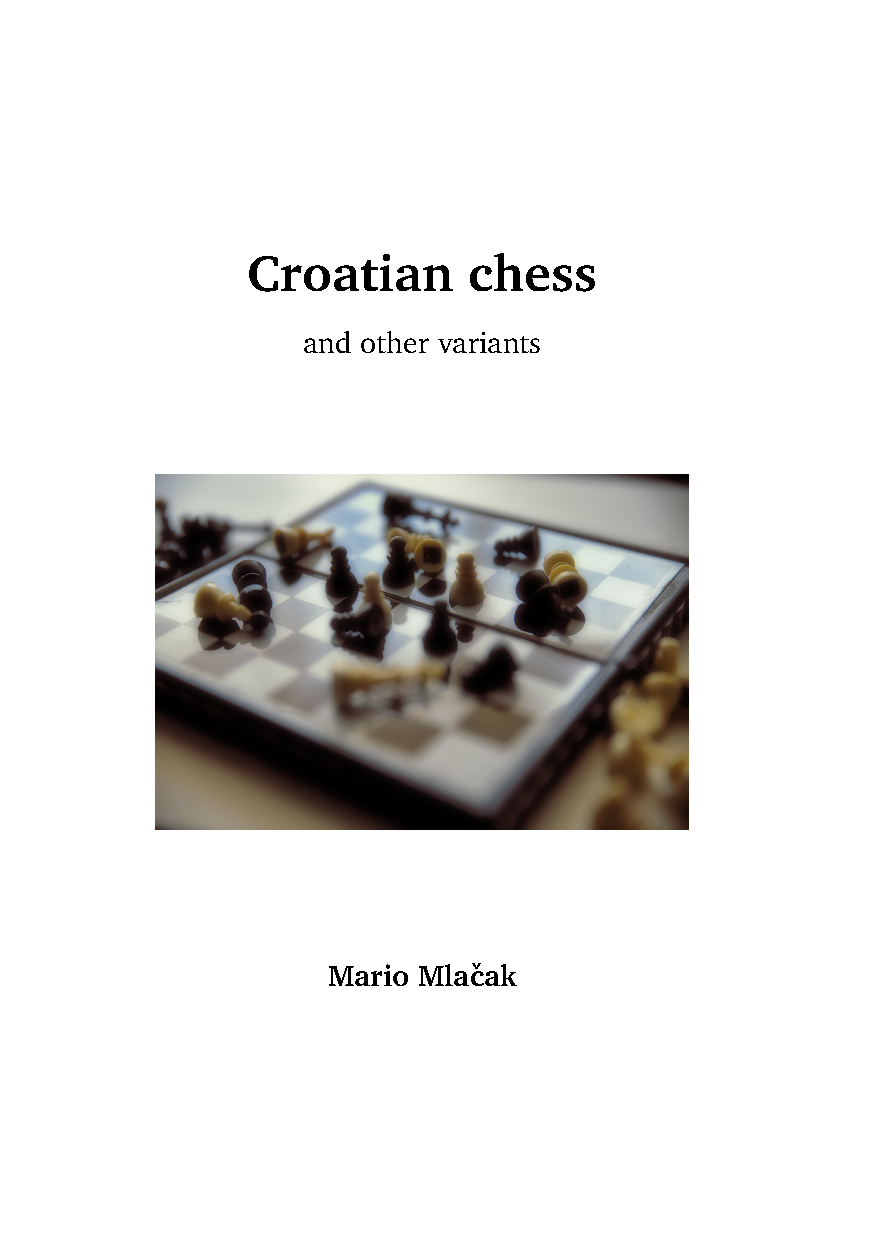
\includegraphics[width=0.8\textwidth, keepaspectratio=true]{crochess.jpg} \\ [2.0cm]

    \textbf{\large{Mario Mlačak}} \\ [2.0cm]
\end{center}
\vspace{\stretch{1}}
\end{titlepage}
% ---------------------------------------------------------- Title page

% Empty page ----------------------------------------------------------
\thispagestyle{empty}
\vspace*{0.1\textheight}
\clearpage % ..........................................................
% ---------------------------------------------------------- Empty page

% Dedication page -----------------------------------------------------
\thispagestyle{empty}
\vspace*{0.2\textheight}
\hfill{Dedicated to Miranda.}
\clearpage % ..........................................................
% ----------------------------------------------------- Dedication page

% Publisher page ------------------------------------------------------
\thispagestyle{empty}
\vspace*{0.05\textheight}
\begin{center}
    \emph{Mario Mlačak} \\
    \textbf{Croatian chess} \\
    and other variants \\ [2.0em]

    \emph{Copyright} \\
    Copyright \copyright \hspace{0.2ex} 2009 -- 2020 Mario Mlačak \\
    \href{mailto:mmlacak@gmail.com}{mmlacak@gmail.com} \\ [2.0em]

    \emph{Source} \\
    \href{https://github.com/mmlacak/crochess}{https://github.com/mmlacak/crochess} \\
    644 \textperiodcentered \textperiodcentered \textperiodcentered ~2020-07-04 10:32:40 UTC \textperiodcentered \textperiodcentered \textperiodcentered ~master \\ [2.0em] % new-commit-count-date-time-branch-place-marker

    \emph{Legal} \\
    This book is published as Public Domain work. \\
    \href{https://en.wikipedia.org/wiki/Public\_domain}{https://en.wikipedia.org/wiki/Public\_domain} \\ [2.0em]

    \emph{Third, revised edition} \\
    2020-07-04 \\ % new-commit-date-place-marker
    Zagreb, Croatia

    \vfill

    \tiny{
        \emph{Parent commit} \\
        b3e48f3c59454af7a451b2f166db9417d151ec82 \\ % last-commit-id-place-marker
        2020-07-04 09:59:19 UTC \\ % last-commit-date-time-place-marker
    }
    \normalsize{}
    \vspace{0.05\textheight}
\end{center}
\clearpage % ..........................................................
% ------------------------------------------------------ Publisher page

% Inner title page ----------------------------------------------------
\thispagestyle{empty}
\vspace*{0.2\textheight}
\begin{center}
    \textbf{\Large{Croatian chess}} \\ [1.0em]
    \large{and other variants} \\ [1.0em]
    \small{3rd, revised edition} \\ [2.0cm]
    \vspace*{0.2\textheight}

    \textbf{\large{Mario Mlačak}} \\ [1.0em]
    \small{2020-07-04} \\ [0.5em] % new-commit-date-small-place-marker
    \small{Zagreb, Croatia}
\end{center}
\clearpage % ..........................................................
% ---------------------------------------------------- Inner title page

% Empty page ----------------------------------------------------------
\thispagestyle{empty}
\vspace*{0.1\textheight}
\clearpage % ..........................................................
% ---------------------------------------------------------- Empty page

% Gratitude page ------------------------------------------------------
\thispagestyle{empty}
\vspace*{0.2\textheight}
\begin{flushright}
My most sincere gratitude to:

Valentina Štefanić \\
Kristina Mlačak \\
Slavko Štefanić

and many, many others.

Thank you all.
\end{flushright}
\clearpage % ..........................................................
% ------------------------------------------------------ Gratitude page

% Empty page ----------------------------------------------------------
\thispagestyle{empty}
\vspace*{0.1\textheight}
\clearpage % ..........................................................
% ---------------------------------------------------------- Empty page

% Introduction chapter ------------------------------------------------

% Copyright (c) 2015 - 2019 Mario Mlačak, mmlacak@gmail.com
% Public Domain work, under CC0 1.0 Universal Public Domain Dedication. See LICENSING, COPYING files for details.

% Introduction chapter ------------------------------------------------
\chapter*{Introduction}
\addcontentsline{toc}{chapter}{Introduction}
\label{ch:Introduction}

\begin{flushright}
\parbox{0.6\textwidth}{
\emph{Life's too short for chess. \newline
\hspace*{\fill}{\textperiodcentered \textperiodcentered \textperiodcentered \hspace*{0.2em} Henry James Byron} } }
\end{flushright}

\noindent
I was in my aunt's house, on the border of a small village.
Through window, walled garden was visible just behind the house.
Behind the garden, a tiny brook. And hills behind the brook.
Afternoon Sun was casting its orange rays into warm room. It
was frosty outside.

My cousin approached me with some nifty gizmo. He was a
few years older than me and was already going to school.

\noindent
"Here, look at what I got." \newline
\hspace*{\fill}"What's that?" \newline
"Chess set. Wanna try? Lemme show you." \newline
\hspace*{\fill}"Sure."

It was small, plasticky, fiddly thing designed to fit into winter's
coat pocket, to be used on the go. Folding board was also used to
hold all pieces in it. Each piece was as small as humanely usable.
Each field had a hole in the middle. At the bottom of each piece
there was small rod fitting into those holes. It was colored all
in red and ivory.

Short lesson revealed it's not that difficult to grasp what's going
on. Within minutes I picked it up. First match was, predictably, a
complete disaster. On the second go my cousin forgot about a piece,
and I grabbed his Queen gleefully. He surrendered.

After he left me with a new widget, I was intrigued. I wasn't
about playing the game, though. I was more into redesign it. Could it
be made better, more challenging, or just different?

\noindent
'Why not make Knight jump longer, say 3 by 1 fields?' \newline
'Hmmmm...' \newline
'Nah, that would make jump too long for such a small board.'

Outside, the setting Sun was shining red.

\vspace*{1.1\baselineskip}
\begin{flushright}
\parbox{0.6\textwidth}{
\emph{ \hspace*{\fill}{late November, 1975} \newline
\hspace*{\fill}{Bednja, Croatia} } }
\end{flushright}

\clearpage % ..........................................................
% ------------------------------------------------ Introduction chapter

% ------------------------------------------------ Introduction chapter

% Prerequisites chapter -----------------------------------------------

% Prerequisites chapter -----------------------------------------------
\chapter*{Prerequisites}
\addcontentsline{toc}{chapter}{Prerequisites}

\begin{flushright}
\parbox{0.7\textwidth}{
\emph{It does not matter how slowly you go as long as you do not stop. \\
\hspace*{\fill}{\textperiodcentered \textperiodcentered \textperiodcentered \hspace*{0.2em} Confucius} } }
\end{flushright}

\noindent
This document describes new variants of chess, new pieces
and rules. In this document I'll describe only even variants, since
generating odd ones from there is an exercise in simplicity. Please,
see 'Even variant', 'Odd variant' in the Definitions bellow.

\textbf{\huge{TODO :: FIX ME !!!}} % TODO :: FIX ME !!!

In this document I'm assuming you have the complete prior
knowledge of classical chess pieces and rules. If not, please visit
Wikipedia entry on this subject at \\
\href{https://en.wikipedia.org/wiki/Rules\_of\_chess}{https://en.wikipedia.org/wiki/Rules\_of\_chess}.
\clearpage
% ----------------------------------------------- Prerequisites chapter


% ----------------------------------------------- Prerequisites chapter

% Classical Game chapter ----------------------------------------------

% Copyright (c) 2015 - 2019 Mario Mlačak, mmlacak@gmail.com
% Published as Public Domain work, under CC0 1.0 Universal Public Domain Dedication. See LICENSING, COPYING files for details.

% Classical Chess -----------------------------------------------------
\chapter*{Classical Chess}
\addcontentsline{toc}{chapter}{Classical Chess}
\label{ch:Classical Chess}

\begin{flushright}
\parbox{0.8\textwidth}{
\emph{A great war leaves the country with three armies -
an army of cripples, an army of mourners, and an army of thieves. \newline
\hspace*{\fill}{\textperiodcentered \textperiodcentered \textperiodcentered \hspace*{0.2em} German proverb} } }
\end{flushright}

\noindent
About Classical Chess is written really everything already, and I have
nothing to add, except to use it as an example on how to read the book.

\clearpage % ..........................................................
% Pieces **************************************************************

\section*{Pieces}
\addcontentsline{toc}{section}{Pieces}
\label{sec:Classical Chess/Pieces}

The easiest way to introduce readers to the rendering of classical pieces
is to show chessboard with initial setup:

\noindent
\begin{figure}[!h]
\includegraphics[width=1.0\textwidth, keepaspectratio=true]{boards/02_classical.png}
\caption{Classical Chess, initial setup}
\label{fig:02_classical}
\end{figure}

\noindent
You can compare this with official rendering at \algfmt{FIDE~2.3}.

\clearpage % ..........................................................

\subsection*{Bishop}
\addcontentsline{toc}{subsection}{Bishop}
\label{sec:Classical Chess/Pieces/Bishop}

\noindent
\begin{wrapfigure}[12]{l}{0.4\textwidth}
\centering
\includegraphics[width=0.4\textwidth, keepaspectratio=true]{pieces/bishop/02_classical.png}
\caption{Bishop}
\label{fig:bishop/02_classical}
\end{wrapfigure}
New pieces are introduced with zoomed-in image, on a \mbox{2 $\times$ 2} board.
Light pieces are rendered on a lower row, dark pieces are on an upper row,
regardless of actual colors used in a particular variant. % \newline
% \indent

Light fields are always in lower-right and upper-left corner, while dark fields
are always in lower-left and upper-right corner, regardless which actual colors
are used to paint board.

% ************************************************************** Pieces
% \clearpage % ..........................................................
% Chessboard **********************************************************

\section*{Chessboard}
\addcontentsline{toc}{section}{Chessboard}
\label{sec:Classical Chess/Chessboard}

As seen on the chessboard on previous page, light player starts from bottom of
a chessboard, while dark player starts from top. This arrangement is used by FIDE
(see \algfmt{FIDE~2.3}), and also for all the examples in this book, and for all
new variants, regardless the size of a chessboard used in a variant.

In such a setup, color of lower-right (and upper-left) corner are determined by
FIDE to be light colored, see \algfmt{FIDE~2.1}; this also applies to all new
variants, regardless which actual colors are used to paint chessboards.

In FIDE handbook, and elsewhere, chessboard is made of \mbox{8 $\times$ 8} grid
of squares; in this book squares are referred to as fields.

\clearpage % ..........................................................
% Examples ============================================================

\subsection*{Examples}
\addcontentsline{toc}{subsection}{Examples}
\label{sec:Classical Chess/Chessboard/Examples}

\vspace*{-0.7\baselineskip}
\noindent
\begin{wrapfigure}[1]{l}{0.4\textwidth}
\centering
\includegraphics[width=0.4\textwidth, keepaspectratio=true]{examples/02_c/scn_cc_01_rook_not_blocked.png}
\vspace*{-1.4\baselineskip}
\caption{Rook not blocked}
\label{fig:scn_cc_01_rook_not_blocked}
\end{wrapfigure}
. . .

\vspace*{13.7\baselineskip}
\noindent
\begin{wrapfigure}[1]{l}{0.4\textwidth}
\centering
\includegraphics[width=0.4\textwidth, keepaspectratio=true]{examples/02_c/scn_cc_02_rook_blocked.png}
\vspace*{-1.4\baselineskip}
\caption{Rook blocked}
\label{fig:scn_cc_02_rook_blocked}
\end{wrapfigure}
. . .

\clearpage % ..........................................................

\vspace*{-1.4\baselineskip}
\noindent
\begin{wrapfigure}[1]{l}{0.4\textwidth}
\centering
\includegraphics[width=0.4\textwidth, keepaspectratio=true]{examples/02_c/scn_cc_03_rook_capturing.png}
\vspace*{-1.4\baselineskip}
\caption{Rook capturing}
\label{fig:scn_cc_03_rook_capturing}
\end{wrapfigure}
. . .

\vspace*{13.7\baselineskip}
\noindent
\begin{wrapfigure}[1]{l}{0.4\textwidth}
\centering
\includegraphics[width=0.4\textwidth, keepaspectratio=true]{examples/02_c/scn_cc_04_rook_diagonal.png}
\vspace*{-1.4\baselineskip}
\caption{Rook diagonal}
\label{fig:scn_cc_04_rook_diagonal}
\end{wrapfigure}
. . .


% ============================================================ Examples
% ********************************************************** Chessboard
\clearpage % ..........................................................

\noindent
\TODO :: introduction \newline

\noindent
\textrightarrow basic terminology: turn, move, cycle, figure, ... \newline
\textrightarrow new terminology: rush, steps, step-fields, capture-fields \newline
\textrightarrow conflicting terminology: activating a piece, ply (?) \newline

\noindent
\textrightarrow arrows \& colors \newline
\textrightarrow markers, texts (enumerations vs. labels) \newline
\textrightarrow navigation \newline

\noindent
\textrightarrow context, exceptions \newline

\clearpage % ..........................................................
% ----------------------------------------------------- Classical Chess

% ---------------------------------------------- Classical Game chapter

% Croatian Ties chapter -----------------------------------------------

% Copyright (c) 2015 - 2020 Mario Mlačak, mmlacak@gmail.com
% Public Domain work, under CC0 1.0 Universal Public Domain Dedication. See LICENSING, COPYING files for details.

% Croatian Ties chapter ===============================================
\chapter*{Croatian Ties}
\addcontentsline{toc}{chapter}{Croatian Ties}
\label{ch:Croatian Ties}

\begin{flushright}
\parbox{0.7\textwidth}{
\emph{Secrecy is the first essential in affairs of the State.\newline
\hspace*{\fill}{\textasciitilde{} De Richelieu} } }
\end{flushright}

\noindent
Croatian Ties is chess variant which is played on 10 $\times$ 10 board,
with light grey and red fields and dark gray and dark red pieces.
A new piece is introduced, Pegasus.

\clearpage % ..........................................................
% Pegasus *************************************************************

\section*{Pegasus}
\addcontentsline{toc}{section}{Pegasus}
\label{sec:Croatian Ties/Pegasus}

\noindent
\begin{wrapfigure}[6]{l}{0.4\textwidth}
\centering
\includegraphics[width=0.4\textwidth, keepaspectratio=true]{pieces/07_pegasus.png}
\caption{Pegasus}
\label{fig:07_pegasus}
\end{wrapfigure}
Pegasus moves similarly to Knight, but it can continue its jumpy movement
until another piece is encountered, or it runs out of board. Note that once
in movement, Pegasus cannot change its heading.

\vspace{5.0\baselineskip}
\subsection*{Movement}
\addcontentsline{toc}{subsection}{Movement}
\label{sec:Croatian Ties/Pegasus/Movement}

\noindent
\begin{wrapfigure}[15]{l}{0.5\textwidth}
\centering
\includegraphics[width=0.5\textwidth, keepaspectratio=true]{examples/04_ct/scn_ct_01_pegasus_initial.png}
\caption{Pegasus initial step}
\label{fig:scn_ct_01_pegasus_initial}
\end{wrapfigure}
In the example on the left we have Pegasus with all valid initial moves marked.
These all are the same as valid moves for Knight.

Pegasus' movement is not hampered by a piece placed on any unmarked field.
Pegasus can "jump" over it just as Knight would.

\clearpage % ..........................................................

\noindent
\begin{figure}[!h]
\includegraphics[width=1.0\textwidth, keepaspectratio=true]{examples/04_ct/scn_ct_02_pegasus_direction.png}
\caption{Pegasus move direction}
\label{fig:scn_ct_02_pegasus_direction}
\end{figure}

Once direction is chosen Pegasus can continue its movement performing one jump
after another in order from nearest field to furthest. Here, this is marked
with green arrows. Accessible fields are marked 1 to 4, in order of accessibility,
from nearest to furthest. Again, once direction is chosen it can't be changed anymore.
For instance, after reaching field 2 it's illegal to change direction to 2f (or
any other red arrow).

\clearpage % ..........................................................

\subsection*{Steps, step-fields, capture-fields, ply}
\addcontentsline{toc}{subsection}{Steps, step-fields, capture-fields, ply}
\label{sec:Croatian Ties/Pegasus/Steps, step-fields, capture-fields, ply}

\noindent
\begin{figure}[!h]
\vspace{-1.0\baselineskip}
\includegraphics[width=1.0\textwidth, keepaspectratio=true]{examples/04_ct/scn_ct_03_define_step_ply.png}
\caption{Step-fields, capture-fields, ply}
\label{fig:scn_ct_03_define_step_ply}
\end{figure}

Above, field 3 is chosen as destination for Pegasus' movement. Move along arrow is a step.
Field at which arrow points to is a step-field. Here, each step-field is also capture-field,
Pegasus would be able to capture opponent's piece on it. Completed movement of Pegasus,
from its starting position to its destination field 3 is a ply.

\clearpage % ..........................................................

\subsection*{Movement (cont.)}
\addcontentsline{toc}{subsection}{Movement (cont.)}
\label{sec:Croatian Ties/Pegasus/Movement (cont.)}

\noindent
\begin{figure}[!h]
\vspace{-1.2\baselineskip}
\includegraphics[width=1.0\textwidth, keepaspectratio=true]{examples/04_ct/scn_ct_04_pegasus_movement.png}
\caption{Pegasus moves}
\label{fig:scn_ct_04_pegasus_movement}
\end{figure}

Pegasus can "jump" over pieces on non-step-fields, Rooks in example above. Numbers
here enumerate directions of movement. Own piece on step-field stops Pegasus at
preceding step-field, see direction 2. Opponent's piece on step-field can be captured
(blue arrow). Just as with any other piece that would finish the move, meaning Pegasus
would have to stop at captured field, see direction 1.

% ************************************************************* Pegasus
\clearpage % ..........................................................

\section*{Rush, en passant}
\addcontentsline{toc}{section}{Rush, en passant}
\label{sec:Croatian Ties/Rush, en passant}

\noindent
\begin{wrapfigure}{l}{0.4\textwidth}
\centering
\includegraphics[width=0.33\textwidth, keepaspectratio=true]{en_passants/04_croatian_ties_en_passant.png}
\caption{En passant}
\label{fig:04_croatian_ties_en_passant}
\end{wrapfigure}
Rush is Pawn's longer initial movement, i.e. from its starting position, for at least
2 fields forward.

Rush and en passant are identical to those in Classic Chess, only difference is that Pawn
can now move longer on initial turn, up to 3 fields in this instance.

In the example on the left, rush fields are numbered. Longer rush also opens more opportunity
for opponent to perform en passant or block it, entirely or partially. For discussion on the
topic see:
\href{https://en.wikipedia.org/wiki/En\_passant}{https://en.wikipedia.org/wiki/En\_passant}.

\clearpage % ..........................................................

\section*{Castling}
\addcontentsline{toc}{section}{Castling}
\label{sec:Croatian Ties/Castling}

\vspace*{-0.3\baselineskip}
Castling is the same as in Classical Chess, only difference is that King can move either 2 or 3
fields across. All other constraints from Classical Chess still applies, described in detail here:
\href{https://en.wikipedia.org/wiki/Castling}{https://en.wikipedia.org/wiki/Castling}.

\vspace*{-0.3\baselineskip}
\noindent
\begin{figure}[!h]
\includegraphics[width=1.0\textwidth, keepaspectratio=true]{castlings/04_ct/croatian_ties_castling.png}
\vspace*{-1.4\baselineskip}
\caption{Castling}
\label{fig:croatian_ties_castling}
\end{figure}

\vspace*{-0.3\baselineskip}
In example above, all valid King's castling moves are numbered. Regardless if castling is long or short,
Rook always ends up on the opposite side of King on the field immediately next to it, i.e. one field closer
to center.

\vspace*{-0.3\baselineskip}
\noindent
\begin{figure}[!h]
\includegraphics[width=1.0\textwidth, keepaspectratio=true]{castlings/04_ct/croatian_ties_castling_left_03.png}
\vspace*{-1.4\baselineskip}
\caption{Castling long left}
\label{fig:croatian_ties_castling_left_03}
\end{figure}

\vspace*{-0.7\baselineskip}
\noindent
\begin{figure}[!h]
\includegraphics[width=1.0\textwidth, keepaspectratio=true]{castlings/04_ct/croatian_ties_castling_right_02.png}
\vspace*{-1.4\baselineskip}
\caption{Castling short right}
\label{fig:croatian_ties_castling_right_02}
\end{figure}

\vspace*{-0.3\baselineskip}
In examples above initial King's position is marked with "K". In both cases, Rook ends up at the
inside field, immediately next to the King.

\clearpage % ..........................................................

\section*{Initial setup}
\addcontentsline{toc}{section}{Initial setup}
\label{sec:Croatian Ties/Initial setup}

Compared to initial setup of Classical Chess, Pegasus is inserted between Rook and Knight
symmetrically, on both sides of chessboard. This can be seen in the image below:

\noindent
\begin{figure}[h]
\includegraphics[width=1.0\textwidth, keepaspectratio=true]{boards/04_croatian_ties.png}
\caption{Croatian Ties board}
\label{fig:04_croatian_ties}
\end{figure}

\clearpage % ..........................................................
% =============================================== Croatian Ties chapter

% ----------------------------------------------- Croatian Ties chapter

% Mayan Ascendancy chapter --------------------------------------------

% Mayan Ascendancy chapter --------------------------------------------
\chapter*{Mayan Ascendancy}
\addcontentsline{toc}{chapter}{Mayan Ascendancy}

\begin{flushright}
\parbox{0.8\textwidth}{
\emph{The world has achieved brilliance without wisdom, power without
conscience. Our is a world of nuclear giants and ethical infants. \\
\hspace*{\fill}{\textperiodcentered \textperiodcentered \textperiodcentered \hspace*{0.2em} Omar Nelson Bradley} } }
\end{flushright}

\noindent
Mayan Ascendancy is chess variant which is played on 12 x 12 board with
yellow and blue fields and with dark yellow and dark blue pieces. In
algebraic notation, columns are enumerated from 'a' to 'l', and rows are
enumerated from '1' to '12'. A new piece is introduced, Pyramid.

\clearpage % ..........................................................

\section*{Pyramid}
\addcontentsline{toc}{section}{Pyramid}

\noindent
\begin{wrapfigure}[12]{l}{0.4\textwidth}
\includegraphics[width=0.4\textwidth, keepaspectratio=true]{pieces/08_pyramid.png}
\caption{Pyramid}
\label{fig:pyramid}
% % \centering
\end{wrapfigure}
Pyramid is passive piece, meaning it can't move on its' own, it has to be
activated first. This is done by capturing a field at which Pyramid stands
with own other piece and then Pyramid can move further.

Once activated Pyramid moves similar to Rook, only real difference is that
it can move for only so many fields as piece activating it has moved, i.e.
for at most as momentum received.

Pyramid can't check opponent's King, and consequently can't contribute to
checkmate. Pyramid can capture all the other opponent's pieces after it has
been activated.

In algebraic notation symbol for Pyramid is 'A', to avoid confusion with Pawn.

\subsection*{Momentum}
\addcontentsline{toc}{subsection}{Momentum}

Momentum is count of step-fields traveled over by a piece. Pyramid receives
momentum from piece which activates it. Momentum is spent by Pyramid when
moving, one for each step-field travelled. So Pyramid can't move for more
fields than received momentum, i.e. for more than activating piece has
travelled. Momentum can't be saved for later, it is wasted when Pyramid
moves for less than received momentum.

\clearpage % ..........................................................

\subsection*{Activation}
\addcontentsline{toc}{subsection}{Activation}

\noindent
\begin{figure}[!h]
% \begin{figure}[!t]
\includegraphics[width=1.0\textwidth, keepaspectratio=true]{examples/06_move_pyramid_activation_init.png}
\caption{Pyramid activation}
\label{fig:ma_activation_init}
% \centering
\end{figure}

Here Pegasus is about to capture field on which Pyramid stands. Note, only
step-fields are counted towards momentum. After activation Pyramid would be
limited to move at most 4 fields across, i.e. at most the momentum it received
from Pegasus.

\clearpage % ..........................................................

\noindent
\begin{figure}[!h]
% \begin{figure}[!t]
\includegraphics[width=1.0\textwidth, keepaspectratio=true]{examples/06_move_pyramid_activated.png}
\caption{Pyramid activated}
\label{fig:ma_activation_ongoing}
% \centering
\end{figure}

Above, arrows show all possible moves by Pyramid. Just like Rook, Pyramid has to
stop before own Bishop. Pyramid can also capture opponent's Rook, but can't move
any further after that.

\clearpage % ..........................................................

\noindent
\begin{figure}[!h]
% \begin{figure}[!t]
\includegraphics[width=1.0\textwidth, keepaspectratio=true]{examples/06_move_pyramid_activation_end.png}
\caption{Pyramid activation end}
\label{fig:ma_activation_end}
% \centering
\end{figure}

Here, Pyramid movement ends by capturing opponent's Knight, which also ends light
player's complete move.

\clearpage % ..........................................................

\subsection*{Promotion}
\addcontentsline{toc}{subsection}{Promotion}

Pyramid can promote own Pawns, but only on opponent's side of the board.
Promotion is done by activating Pyramid which then marks Pawn for promotion
by touching either Pawn or field at which it stands. Pyramid then leaves
board as if it was captured, and Pawn is replaced by desired piece, for
instance Queen.

Both Pyramid and Pawn in question has to reside on opponent's side of the
board before promotion can take place. Piece which activates Pyramid need
not to be on opponent's side of the board.

Piece which Pawn can be promoted to is from the set of all starting pieces,
except King. This promoting-to piece is not limited to pieces already being
captured.

\clearpage % ..........................................................

\noindent
% \begin{figure}[!h]
\begin{figure}[!t]
\includegraphics[width=1.0\textwidth, keepaspectratio=true]{examples/06_move_pyramid_promo_init.png}
\caption{Promotion start}
\label{fig:ma_promo_init}
% \centering
\end{figure}

Here, Pegasus is accumulating momentum while travelling over step-fields. After
activation Pyramid would be limited to move at most 4 fields across, i.e. at most
the momentum it received from Pegasus.

\clearpage % ..........................................................

\noindent
% \begin{figure}[!h]
\begin{figure}[!t]
\includegraphics[width=1.0\textwidth, keepaspectratio=true]{examples/06_move_pyramid_promo_activate.png}
\caption{Promotion, Pyramid activated}
\label{fig:ma_promo_activate}
% \centering
\end{figure}

Above, Pegasus captured field at which Pyramid was situated, arrows now show
all possible moves by Pyramid. Only full move to the right leads to promotion,
shown in red. Just as Rook, Pyramid can't advance past Pawn.

\clearpage % ..........................................................

\noindent
% \begin{figure}[!h]
\begin{figure}[!t]
\includegraphics[width=1.0\textwidth, keepaspectratio=true]{examples/06_move_pyramid_promo_end.png}
\caption{Promotion end}
\label{fig:ma_promo_end}
% \centering
\end{figure}

Now that Pyramid has reached Pawn, it is removed from the board and piece of
choice, in this instance Queen, replaces Pawn.

\clearpage % ..........................................................

\subsection*{Conversion}
\addcontentsline{toc}{subsection}{Conversion}

Pyramid can convert opponent's pieces, except King, but only on own side of
the board. Conversion is done by activating Pyramid which then marks opponent's
piece for conversion by touching either piece or field at which it stands. Now
Pyramid leaves the board as if it was captured, and opponent's piece is replaced
by own piece of the same type.

Both Pyramid and opponent's piece has to reside on own side of the board
before conversion can take place. Piece which activates Pyramid need not
to be on own side of the board. As with promotion, conversion is not limited
to pieces which has been captured.

Note that Pyramid might just as well capture opponent's piece. Differences are
who leaves chess board, and what remains on captured field. Capture itself with
Pyramid is in no way different than that with Rook, provided that Pyramid can
reach opponent's piece, i.e. that it get enough momentum from activating piece.

\clearpage % ..........................................................

\noindent
% \begin{figure}[!h]
\begin{figure}[!t]
\includegraphics[width=1.0\textwidth, keepaspectratio=true]{examples/06_move_pyramid_conversion_init.png}
\caption{Conversion start}
\label{fig:ma_conversion_init}
% \centering
\end{figure}

For classic pieces, step-fields are just fields which piece traveled over,
in case of Bishop above that is 4 fields. Again, that is momentum Pyramid
will receive with activation and limits how far it could move afterwards.

\clearpage % ..........................................................

\noindent
% \begin{figure}[!h]
\begin{figure}[!t]
\includegraphics[width=1.0\textwidth, keepaspectratio=true]{examples/06_move_pyramid_conversion_activated.png}
\caption{Conversion, Pyramid activated}
\label{fig:ma_conversion_activated}
% \centering
\end{figure}

Above, Bishop captured field at which Pyramid was situated, arrows now show
all possible moves by Pyramid. Only full move to the right leads to conversion,
shown in red. Again, just as Rook, Pyramid can't advance past opponent's Rook.

\clearpage % ..........................................................

\noindent
% \begin{figure}[!h]
\begin{figure}[!t]
\includegraphics[width=1.0\textwidth, keepaspectratio=true]{examples/06_move_pyramid_conversion_end.png}
\caption{Conversion end}
\label{fig:ma_conversion_end}
% \centering
\end{figure}

Now that Pyramid has reached opponent's Rook, it is removed from the board and
own Rook replaces opponent's Rook. Capturing opponent's Rook would simply leave
Pyramid in place of it.

\clearpage % ..........................................................

\subsection*{Cascading}
\addcontentsline{toc}{subsection}{Cascading}

\noindent
\begin{figure}[!h]
% \begin{figure}[!t]
\includegraphics[width=1.0\textwidth, keepaspectratio=true]{examples/06_move_pyramid_cascading_init.png}
\caption{Cascading start}
\label{fig:ma_cascading_init}
% \centering
\end{figure}

Once activated, Pyramid can also activate another Pyramid. To do so, activated
Pyramid has to have at least 1 remaining momentum to transfer it to another
Pyramid. If all momentum received was spent moving, Pyramid cannot activate
another Pyramid.

\clearpage % ..........................................................

\noindent
\begin{figure}[!h]
% \begin{figure}[!t]
\includegraphics[width=1.0\textwidth, keepaspectratio=true]{examples/06_move_pyramid_cascading_activated_1.png}
\caption{Cascading, 1st Pyramid activated}
\label{fig:ma_cascading_1}
% \centering
\end{figure}

Pyramid 1 has been activated by Queen and received momentum of 5, arrows now show
its' all possible moves. Note, Pyramid 3 can't be activated, it's on the very end
of fields reachable by Pyramid 1.

\clearpage % ..........................................................

\noindent
\begin{figure}[!h]
% \begin{figure}[!t]
\includegraphics[width=1.0\textwidth, keepaspectratio=true]{examples/06_move_pyramid_cascading_activated_2.png}
\caption{Cascading, 2nd Pyramid activated}
\label{fig:ma_cascading_2}
% \centering
\end{figure}

Pyramid 2 has been activated by Pyramid 1 and in the process received momentum of 2,
arrows now show all possible moves by Pyramid 2.

\clearpage % ..........................................................

\noindent
\begin{figure}[!h]
% \begin{figure}[!t]
\includegraphics[width=1.0\textwidth, keepaspectratio=true]{examples/06_move_pyramid_cascading_end.png}
\caption{Cascading end}
\label{fig:ma_cascading_end}
% \centering
\end{figure}

Pyramid 2 has finished its' movement, and so it ends light player's complete move.

\clearpage % ..........................................................

\subsection*{Against King}
\addcontentsline{toc}{subsection}{Against King}

Pyramid can't check opponent's King, meaning that King is not under attack
even if Pyramid could capture any other piece on the same field.

\noindent
\begin{figure}[!h]
% \begin{figure}[!t]
\includegraphics[width=1.0\textwidth, keepaspectratio=true]{examples/06_move_pyramid_vs_king.png}
\caption{Pyramid vs. King}
\label{fig:pyramid_vs_king}
% \centering
\end{figure}

Above, King is not under attack from Pyramid.

\noindent
\begin{figure}[!h]
% \begin{figure}[!t]
\includegraphics[width=1.0\textwidth, keepaspectratio=true]{examples/06_move_pyramid_vs_bishop.png}
\caption{Pyramid vs. Bishop}
\label{fig:pyramid_vs_bishop}
% \centering
\end{figure}

Bishop in the same place, however, could be captured without any hindrance.

\clearpage % ..........................................................

\subsection*{Activation by Pawn}
\addcontentsline{toc}{subsection}{Activation by Pawn}

\noindent
\begin{figure}[!h]
% \begin{figure}[!t]
\includegraphics[width=1.0\textwidth, keepaspectratio=true]{examples/06_move_pyramid_activation_by_pawn.png}
\caption{Pyramid activation by Pawns}
\label{fig:ma_activation_by_pawns}
% \centering
\end{figure}

Capture-fields are all fields where a piece can capture opponents' piece.
Usually these are the same as step-fields, except for Pawn. Pawns can activate
Pyramid on own capture-field giving it 1 momentum (1). Pawns can't activate
Pyramids on step-fields, and are blocked from moving further (2, 3).

\clearpage % ..........................................................

\section*{En passant}
\addcontentsline{toc}{section}{En passant}

\noindent
\begin{wrapfigure}{l}{0.4\textwidth}
\includegraphics[width=0.4\textwidth, keepaspectratio=true]{en_passants/06_mayan_ascendancy_en_passant.png}
\caption{En passant}
\label{fig:ma_en_passant}
% % \centering
\end{wrapfigure}
En passant is identical to one in Classic Chess, only difference is that Pawn can now
move longer on initial turn, up to 4 fields in this instance. As expected, all passed-by
opponent's Pawns also gain en passant opportunity.

In example on left, if light Pawn's initial move was 3 fields long, ending in field marked
2, two dark Pawns closest to light Pawn's initial position would have en passant opportunity,
in rows 1 and 2.

\clearpage % ..........................................................

\section*{Castling}
\addcontentsline{toc}{section}{Castling}

Castling is essentially the same as it is in Classical Chess, only real difference is that
King can move 2, 3 or 4 fields across. All other constraints from Classical Chess still
applies.

\noindent
\begin{figure}[!h]
% \begin{figure}[!t]
\includegraphics[width=1.0\textwidth, keepaspectratio=true]{castlings/06_mayan_ascendancy_castling.png}
\caption{Castling}
\label{fig:ma_castling}
% \centering
\end{figure}

In example above, all valid King's castling moves are numbered. Regardless if King performs
long or short castling move, Rook would always end up on the opposite side of King on the
field immediately next to it, i.e. closer to center.

\noindent
\begin{figure}[!h]
% \begin{figure}[!t]
\includegraphics[width=1.0\textwidth, keepaspectratio=true]{castlings/long_left/06_mayan_ascendancy_castling_long_left.png}
\caption{Castling long left}
\label{fig:ma_castling_long_left}
% \centering
\end{figure}

In this example King was castling long to the left. Initial King's position is marked with "K".
After castling is finished, left Rook ends up at field immediately on the right to the King.

\clearpage % ..........................................................

\section*{Initial setup}
\addcontentsline{toc}{section}{Initial setup}

Compared to initial setup of Croatian Ties, Pyramid is inserted between Pegasus and Knight
symmetrically, on both sides of chess board. This can be seen in the image below:

\noindent
% \begin{figure}[t]
\begin{figure}[h]
\includegraphics[width=1.0\textwidth, keepaspectratio=true]{boards/06_mayan_ascendancy.png}
\caption{Mayan Ascendancy board}
\label{fig:mayan_ascendancy}
% \centering
\end{figure}

\clearpage % ..........................................................
% -------------------------------------------- Mayan Ascendancy chapter

% -------------------------------------------- Mayan Ascendancy chapter

% Age of Aquarius chapter ---------------------------------------------

% Copyright (c) 2015 - 2020 Mario Mlačak, mmlacak@gmail.com
% Licensed and published as Public Domain work.

% Age of Aquarius chapter =============================================
\chapter*{Age of Aquarius}
\addcontentsline{toc}{chapter}{Age of Aquarius}

\begin{flushright}
\parbox{0.8\textwidth}{
\emph{The greatest difficulty with the world is not its ability to produce, but the unwillingness to share. \\
\hspace*{\fill}{\textperiodcentered \textperiodcentered \textperiodcentered \hspace*{0.2em} Roy L. Smith} } }
\end{flushright}

\noindent
Age of Aquarius is chess variant which is played on 14 x 14 board,
with light yellow and light green fields and light tan-gold and
dark green pieces. In algebraic notation, columns are enumerated
from 'a' to 'n', and rows are enumerated from '1' to '14'. A new
piece is introduced, Unicorn.

\clearpage % ..........................................................
% Unicorn *************************************************************

\section*{Unicorn}
\addcontentsline{toc}{section}{Unicorn}

\noindent
\begin{wrapfigure}[7]{l}{0.4\textwidth}
\centering
\includegraphics[width=0.4\textwidth, keepaspectratio=true]{pieces/09_unicorn.png}
\caption{Unicorn}
\label{fig:09_unicorn}
\end{wrapfigure}
Unicorn is a piece similar to Knight, only it can jump longer on
opposite color fields. Just as Knight, Unicorn is not obstructed
by any piece in its' surroundings.

In algebraic notation, symbol for Unicorn is 'U'.

\vspace{4\baselineskip}
\subsection*{Movement}
\addcontentsline{toc}{subsection}{Movement}
\label{sec:Age of Aquarius/Unicorn/Movement}

\noindent
\begin{wrapfigure}{l}{0.4\textwidth}
\centering
\includegraphics[width=0.4\textwidth, keepaspectratio=true]{examples/08_aoa/scn_aoa_01_unicorn_same_color.png}
\caption{Unicorn short jump}
\label{fig:scn_aoa_01_unicorn_same_color}
\end{wrapfigure}
On fields with the same color as Unicorn, it can move exactly the
same way Knight does.

\clearpage % ..........................................................

\noindent
\begin{figure}[!h]
% \begin{figure}[!t]
\includegraphics[width=1.0\textwidth, keepaspectratio=true]{examples/08_aoa/scn_aoa_02_unicorn_opposite_color.png}
\caption{Unicorn long jump}
\label{fig:scn_aoa_02_unicorn_opposite_color}
% \centering
\end{figure}

On fields in opposite color, Unicorn can jump much longer. Again, just as
Knight, Unicorn is not hampered by surrounding pieces. Own pieces on marked
step-fields would prevent Unicorn to move. The same marked fields are also
capture-fields, opponent's pieces on them could be captured.

For comparison, Knight's step-fields are also numbered (gray).

% ************************************************************* Unicorn
\clearpage % ..........................................................
% Promotion ***********************************************************

\section*{Promotion}
\addcontentsline{toc}{section}{Promotion}
\label{sec:Age of Aquarius/Promotion}

In all variants prior to this one promotion was forced, Pawn had to be
promoted immediately upon reaching opposite end of chessboard (or when
\hyperref[sec:Mayan Ascendancy/Pyramid/Promotion]{reached by own Pyramid} on
\hyperref[sec:Definitions/Sides of a chessboard]{opponent's side of the board}).
Promotion otherwise is identical to one in Classical Chess, which is
described in details here: \\
\href{https://en.wikipedia.org/wiki/Promotion\_(chess)}{https://en.wikipedia.org/wiki/Promotion\_(chess)}.

In this variant promotion is not forced, Pawn does not have to be promoted
immediately, or at all. Pawn can be promoted later in a game, if it hasn't
moved between being tagged for promotion and actual promotion itself. Thus,
promotion can take place only on a field at which Pawn has been tagged for
promotion.

If tagged Pawn moves before actual promotion, that opportunity has been
lost. Field at which Pawn has been tagged for promotion does not hold tag,
and does not grant ability to promote to any other Pawn passing over it.

Delayed promotion is a complete move, it can contain only promotion of one
Pawn and nothing else.

\clearpage % ..........................................................

\noindent
% \begin{figure}[t]
\begin{figure}[h]
\includegraphics[width=1.0\textwidth, keepaspectratio=true]{examples/08_aoa/scn_aoa_03_delayed_promo_init.png}
\caption{Promotion start}
\label{fig:scn_aoa_03_delayed_promo_init}
% \centering
\end{figure}

Here, light player is about to tag Pawn 2 for promotion, using Pyramid
activated by Bishop. Note, Pawn 3 is not yet eligible for promotion, as it's
still on own side of chessboard.

\clearpage % ..........................................................

\noindent
% \begin{figure}[t]
\begin{figure}[h]
\includegraphics[width=1.0\textwidth, keepaspectratio=true]{examples/08_aoa/scn_aoa_04_delayed_promo_pawn_2_tagged.png}
\caption{Pawn 2 tagged for promotion}
\label{fig:scn_aoa_04_delayed_promo_pawn_2_tagged}
% \centering
\end{figure}

To speed things up, next images show dark player's response (grey arrow),
and light player's plan for next move (green arrow). Each depicted position
is after dark player's move, but before light player's move.

Here, dark Unicorn is attacking tagged Pawn 2. Pawn 2 is to move next.

\clearpage % ..........................................................

\noindent
% \begin{figure}[t]
\begin{figure}[h]
\includegraphics[width=1.0\textwidth, keepaspectratio=true]{examples/08_aoa/scn_aoa_05_delayed_promo_pawn_2_moved.png}
\caption{Pawn 1 about to get promotion}
\label{fig:scn_aoa_05_delayed_promo_pawn_2_moved}
% \centering
\end{figure}

Dark Unicorn closed in, attacking both Pawn 2 and Bishop. Since Pawn 2 moved
away from field P at which it was tagged for promotion, that opportunity has
been lost, and can't be recovered. Label P on a field just marks where Pawn 2
was tagged for promotion. Field P isn't special in any way, it won't make e.g.
Pawn 3 tagged for promotion when reached.

Light Pawn 1 is about to go next.

\clearpage % ..........................................................

\noindent
% \begin{figure}[t]
\begin{figure}[h]
\includegraphics[width=1.0\textwidth, keepaspectratio=true]{examples/08_aoa/scn_aoa_06_delayed_promo_pawn_1_tagged.png}
\caption{Pawn 1 tagged for promotion}
\label{fig:scn_aoa_06_delayed_promo_pawn_1_tagged}
% \centering
\end{figure}

Light Pawn 1 is now tagged for promotion, and is to be promoted later.
Dark Unicorn closed in again, capturing light Bishop.

Light Pawn 2 is about to go next.

\clearpage % ..........................................................

\noindent
% \begin{figure}[t]
\begin{figure}[h]
\includegraphics[width=1.0\textwidth, keepaspectratio=true]{examples/08_aoa/scn_aoa_07_delayed_promo_pawn_1_promoted.png}
\caption{Pawn 1 promoted}
\label{fig:scn_aoa_07_delayed_promo_pawn_1_promoted}
% \centering
\end{figure}

Dark Unicorn captures light Pawn 2.

Light Pawn 1 is promoted to Queen.

% *********************************************************** Promotion
\clearpage % ..........................................................

\section*{Rush, en passant}
\addcontentsline{toc}{section}{Rush, en passant}

\noindent
\begin{wrapfigure}{l}{0.4\textwidth}
\centering
\includegraphics[width=0.214285714286\textwidth, keepaspectratio=true]{en_passants/08_age_of_aquarius_en_passant.png}
\caption{En passant}
\label{fig:08_age_of_aquarius_en_passant}
\end{wrapfigure}
Rush and en passant are identical to those in Classic Chess, only difference
is that Pawn can now move longer on initial turn, up to 5 fields in this
variant.

Converted opponent's Pawns cannot be rushed, even if converted on an initial positions
of own Pawns.

\clearpage % ..........................................................

\section*{Castling}
\addcontentsline{toc}{section}{Castling}

Castling is the same as in Classical Chess, only difference is that King can move 2, 3, 4 or 5 fields across.
All other constraints from Classical Chess still applies.

\noindent
\begin{figure}[!h]
% \begin{figure}[!t]
\includegraphics[width=1.0\textwidth, keepaspectratio=true]{castlings/08_aoa/age_of_aquarius_castling.png}
\caption{Castling}
\label{fig:age_of_aquarius_castling}
% \centering
\end{figure}

In example above, all valid King's castling moves are numbered.

\noindent
\begin{figure}[!h]
% \begin{figure}[!t]
\includegraphics[width=1.0\textwidth, keepaspectratio=true]{castlings/08_aoa/age_of_aquarius_castling_left_04.png}
\caption{Castling long left}
\label{fig:age_of_aquarius_castling_left_04}
% \centering
\end{figure}

In this example King was castling long to the left. Initial King's position is marked with "K".
After castling is finished, left Rook ends up on the field immediately right to the King.

Converted opponent's Rooks cannot be castled, even if converted on an initial positions
of own Rooks.

\clearpage % ..........................................................

\section*{Initial setup}
\addcontentsline{toc}{section}{Initial setup}

Compared to initial setup of Mayan Ascendancy, Unicorn is inserted between Pyramid and Knight
symmetrically, on both sides of chessboard. This can be seen in the image below:

\noindent
% \begin{figure}[t]
\begin{figure}[h]
\includegraphics[width=1.0\textwidth, keepaspectratio=true]{boards/08_age_of_aquarius.png}
\caption{Age of Aquarius board}
\label{fig:08_age_of_aquarius}
% \centering
\end{figure}

\clearpage % ..........................................................
% ============================================= Age of Aquarius chapter

% --------------------------------------------- Age of Aquarius chapter

% Miranda's veil chapter ----------------------------------------------

% Copyright (c) 2015 - 2020 Mario Mlačak, mmlacak@gmail.com
% Public Domain work, under CC0 1.0 Universal Public Domain Dedication. See LICENSING, COPYING files for details.

% Miranda's veil chapter ==============================================
\chapter*{Miranda's veil}
\addcontentsline{toc}{chapter}{Miranda's veil}
\label{ch:Miranda's veil}

\begin{flushright}
\parbox{0.8\textwidth}{
\emph{Under all that we think, lives all we believe, like the ultimate veil of our spirits. \newline
\hspace*{\fill}{\textperiodcentered \textperiodcentered \textperiodcentered \hspace*{0.2em} Antonio Machado} } }
\end{flushright}

\noindent
Miranda's veil is chess variant which is played on 16 x 16 board, with
white and dark violet fields and light magenta and indigo pieces.
A new piece is introduced, Wave.

\clearpage % ..........................................................
% Wave ****************************************************************

\section*{Wave}
\addcontentsline{toc}{section}{Wave}
\label{sec:Miranda's veil/Wave}

\vspace*{-1.4\baselineskip}
\noindent
\begin{wrapfigure}[12]{l}{0.4\textwidth}
\centering
\includegraphics[width=0.4\textwidth, keepaspectratio=true]{pieces/10_wave.png}
\caption{Wave}
\label{fig:10_wave}
\end{wrapfigure}
Wave is passive piece, it has to be activated before it can move. Activation is done
with own piece capturing field at which Wave is located, before Wave can move.
Movement of Wave mimics that of activating piece, and is not limited to a single
step.

Wave does not use received momentum for moving, and so Wave can be activated even
with no momentum. Wave can activate any own piece, except King, if it has momentum.
Wave can also activate other Wave, own or opponent's, even if it has no momentum.
Wave transfers all of received momentum to a piece it activates.

Wave is transparent; all other pieces can move past (pass over) Wave, as if it
isn't present on a chessboard. Other pieces are transparent to Wave; Wave can move
past (pass over) any piece, as if it isn't there. Transparency of Wave makes
activation of Wave optional.

Wave cannot capture any piece; and so cannot neither check nor checkmate opponent's
King.

\clearpage % ..........................................................
% Activation ----------------------------------------------------------

\subsection*{Activation}
\addcontentsline{toc}{subsection}{Activation}
\label{sec:Miranda's veil/Wave/Activation}

\vspace*{-1.4\baselineskip}
\noindent
\begin{figure}[!h]
\includegraphics[width=1.0\textwidth, keepaspectratio=true]{examples/10_mv/scn_mv_01_wave_activation_init.png}
\vspace*{-1.3\baselineskip}
\caption{Activating Wave}
\label{fig:scn_mv_01_wave_activation_init}
\end{figure}

\vspace*{-0.3\baselineskip}
A piece can activate own Wave by simply capturing a field at which that Wave stands.
Activation is optional, a piece could just as well move past Wave. Activated Wave
receives any momentum activating piece had.

Here, Pegasus has opportunity to activate Wave, with 5 momentum.

\clearpage % ..........................................................

\vspace*{-2.1\baselineskip}
\noindent
\begin{figure}[!h]
\includegraphics[width=1.0\textwidth, keepaspectratio=true]{examples/10_mv/scn_mv_02_wave_activated.png}
\caption{Wave activated}
\label{fig:scn_mv_02_wave_activated}
\end{figure}

Activated Wave inherits way of moving from the activating piece. Activated Wave
does not spend received momentum for moving, and so Wave can be activated even if
activating piece has no momentum.

Here, Wave activated by Pegasus (now "in the air") moves like one, i.e. along one
chosen semi-diagonal.

\clearpage % ..........................................................
% Activating pieces ...................................................

\subsubsection*{Activating pieces}
\addcontentsline{toc}{subsubsection}{Activating pieces}
\label{sec:Miranda's veil/Wave/Activation/Activating pieces}

\vspace*{-1.5\baselineskip}
\noindent
\begin{figure}[!h]
\includegraphics[width=1.0\textwidth, keepaspectratio=true]{examples/10_mv/scn_mv_03_pawn_pass_through.png}
\vspace*{-1.4\baselineskip}
\caption{Passing opponent's Pawn}
\label{fig:scn_mv_03_pawn_pass_through}
\end{figure}

\vspace*{-0.5\baselineskip}
Wave in its movement is not obstructed by any piece on chessboard, it can move
past (pass over) any piece, as if it's not there. In short, other pieces are
all transparent to Wave, and all activations are optional.

Here, Wave cannot activate opponent's Pawn on its step-field, but it's not
hindered by that Pawn, and can reach fields behind it, which would be out of
reach for Pegasus.

\clearpage % ..........................................................

\vspace*{-2.1\baselineskip}
\noindent
\begin{figure}[!h]
\includegraphics[width=1.0\textwidth, keepaspectratio=true]{examples/10_mv/scn_mv_04_wave_activating_rook.png}
\vspace*{-1.3\baselineskip}
\caption{Activating Rook}
\label{fig:scn_mv_04_wave_activating_rook}
\end{figure}

\vspace*{-0.3\baselineskip}
Wave can activate any own piece, except King, if it has momentum. Wave can also
activate any other Wave, own or opponent's, even if it doesn't have any momentum.
Wave does not spend received momentum while moving, and would transfer it entirely
to any piece it activates.

Here, Wave can activate own Rook, even though it's positioned behind opponent's
Pawn, and transfer to it all of 5 received momentum.

\clearpage % ..........................................................

\vspace*{-2.1\baselineskip}
\noindent
\begin{figure}[!h]
\includegraphics[width=1.0\textwidth, keepaspectratio=true]{examples/10_mv/scn_mv_05_rook_activated.png}
\vspace*{-1.3\baselineskip}
\caption{Rook activated}
\label{fig:scn_mv_05_rook_activated}
\end{figure}

\vspace*{-0.3\baselineskip}
Material is any piece, except Wave. Activated material moves the same as it would
in a normal move, i.e. if not activated. The only difference is that activated
material is limited by received momentum, i.e. can't move for more fields than
momentum it received.

Here, activated Rook (now "in the air") can choose one of horizontals or verticals
as its new direction. Rook can reach at most 5 fields, because that's the momentum
it received.

\clearpage % ..........................................................

\vspace*{-2.1\baselineskip}
\noindent
\begin{figure}[!h]
\includegraphics[width=1.0\textwidth, keepaspectratio=true]{examples/10_mv/scn_mv_06_rook_captures.png}
% \vspace*{-1.3\baselineskip}
\caption{Rook captures}
\label{fig:scn_mv_06_rook_captures}
\end{figure}

Activated material piece can also capture opponent's piece, if it's within reach,
and not obstructed by other pieces.

Here, activated Rook can capture dark Knight; it can't capture dark Bishop since
own light Pawn is in the way. Light Rook can't capture dark Pegasus since it's out
of reach.

% ................................................... Activating pieces
\clearpage % ..........................................................
% Wave is transparent .................................................

\subsubsection*{Wave is transparent}
\addcontentsline{toc}{subsubsection}{Wave is transparent}
\label{sec:Miranda's veil/Wave/Cascading Waves/Wave is transparent}

\vspace*{-1.4\baselineskip}
\noindent
\begin{figure}[!h]
\includegraphics[width=1.0\textwidth, keepaspectratio=true]{examples/10_mv/scn_mv_07_wave_is_transparent.png}
\vspace*{-1.3\baselineskip}
\caption{Wave is transparent}
\label{fig:scn_mv_07_wave_is_transparent}
\end{figure}

\vspace*{-0.4\baselineskip}
Just as other pieces are transparent to Wave, so is Wave transparent for all the
other pieces. Any interaction with a Wave is optional; a piece could activate own
Wave, it could capture opponent's Wave, or it could move past all Waves in its path,
and e.g. capture opponent's piece behind a Wave.

\noindent
Here, light Queen could interact with any Wave in her path, or capture dark Pegasus;
dark Pawn is shielded by own Pegasus.

\clearpage % ..........................................................

\vspace*{-2.1\baselineskip}
\noindent
\begin{figure}[!h]
\includegraphics[width=1.0\textwidth, keepaspectratio=true]{examples/10_mv/scn_mv_08_wave_cant_be_pinned.png}
\vspace*{-1.3\baselineskip}
\caption{Wave is not pinned}
\label{fig:scn_mv_08_wave_cant_be_pinned}
\end{figure}

\vspace*{-0.5\baselineskip}
Since it's transparent Wave cannot be pinned, i.e. a piece can ignore (pass over)
Wave placed on its capture-field, and still check opponent's King.

Here, dark Pegasus checks light King, even though light Wave is on dark Pegasus'
capture-field. Any other piece positioned instead of light Wave would be
\href{https://en.wikipedia.org/wiki/Pin_(chess)#Absolute_pin}{hard-pinned},
and light King wouldn't be in check.

% ................................................. Wave is transparent
\clearpage % ..........................................................

\subsubsection*{Wave and castling}
\addcontentsline{toc}{subsubsection}{Wave and castling}
\label{sec:Miranda's veil/Wave/Cascading Waves/Wave and castling}

\vspace*{-0.4\baselineskip}
Wave is transparent, so it doesn't block castling if positioned between castling
pieces and their destination fields. Wave cannot be activated by castling piece,
so it blocks any castling which uses its field as a destination.

\vspace*{-0.4\baselineskip}
\noindent
\begin{figure}[!h]
\includegraphics[width=1.0\textwidth, keepaspectratio=true]{examples/10_mv/scn_mv_09_wave_no_block_castling_king.png}
\vspace*{-1.4\baselineskip}
\caption{Castling King}
\label{fig:scn_mv_09_wave_no_block_castling_king}
\end{figure}

\vspace*{-1.4\baselineskip}
\noindent
\begin{figure}[!h]
\includegraphics[width=1.0\textwidth, keepaspectratio=true]{examples/10_mv/scn_mv_10_wave_no_block_castling_rook.png}
\vspace*{-1.4\baselineskip}
\caption{Castling Rook}
\label{fig:scn_mv_10_wave_no_block_castling_rook}
\end{figure}

\vspace*{-0.4\baselineskip}
In previous example King initiated castling by moving onto a field past Wave, Rook
can now finish castling onto empty field between the two, so the whole castling move
is legal.

\vspace*{-0.4\baselineskip}
\noindent
\begin{figure}[!h]
\includegraphics[width=1.0\textwidth, keepaspectratio=true]{examples/10_mv/scn_mv_11_wave_block_castling_rook.png}
\vspace*{-1.4\baselineskip}
\caption{Castling Rook blocked}
\label{fig:scn_mv_11_wave_block_castling_rook}
\end{figure}

\vspace*{-0.4\baselineskip}
If in previous example King initiated castling by moving onto a field just past Wave,
Rook cannot castle onto field occupied by Wave, so the whole castling move is illegal.

\clearpage % ..........................................................

\subsubsection*{Single-step pieces and transparency}
\addcontentsline{toc}{subsubsection}{Single-step pieces and transparency}
\label{sec:Miranda's veil/Wave/Cascading Waves/Single-step pieces and transparency}

\vspace*{-0.7\baselineskip}
\noindent
\begin{wrapfigure}[13]{l}{0.4\textwidth}
\centering
\includegraphics[width=0.39375\textwidth, keepaspectratio=true]{examples/10_mv/scn_mv_12_pawn_blocked_by_opponents_wave.png}
\vspace*{-1.4\baselineskip}
\caption{Pawns blocked by Waves}
\label{fig:scn_mv_12_pawn_blocked_by_opponents_wave}
\end{wrapfigure}
Image on the left and the next one both have two examples presented in parallel,
each started by a labeled Pawn. \newline
\indent
To use transparency, a piece has to be able to reach a Wave, and then make another
step away from it, in the same ply. So, single-step piece (i.e. a Pawn, Knight, King,
or Unicorn) has to activate own, or capture opponent's Wave; otherwise it's blocked
by a Wave, regardless if own, or opponent's.

\vspace*{1.1\baselineskip}
\noindent
\begin{wrapfigure}[16]{l}{0.4\textwidth}
\centering
\includegraphics[width=0.39375\textwidth, keepaspectratio=true]{examples/10_mv/scn_mv_13_pawn_not_blocked_by_opponents_wave.png}
\vspace*{-1.4\baselineskip}
\caption{Pawns not blocked by Waves}
\label{fig:scn_mv_13_pawn_not_blocked_by_opponents_wave}
\end{wrapfigure}
In previous example light Pawn B is blocked from moving straight forward by dark
Wave on its step-field; other Waves can be either activated, or captured. No Wave
can be passed over, since both Pawns can make only one step in a ply. \newline
\indent
Here, both Pawns can rush, thus making more than one step in a single ply. Opponent's,
dark Wave is blocking light Pawn B from settling onto step-field it occupies. Even so,
both Waves are transparent to light Pawns; each Pawn can now pass over corresponding
Wave, and reach step-fields behind it.

\clearpage % ..........................................................

\subsubsection*{Piece blocked}
\addcontentsline{toc}{subsubsection}{Piece blocked}
\label{sec:Miranda's veil/Wave/Activation/Piece blocked}

\vspace*{-1.4\baselineskip}
\noindent
\begin{figure}[h]
\includegraphics[width=1.0\textwidth, keepaspectratio=true]{examples/10_mv/scn_mv_14_wave_no_activating_blocked_piece.png}
\caption{Piece blocked}
\label{fig:scn_mv_14_wave_no_activating_blocked_piece}
\end{figure}

Wave cannot activate blocked pieces, even if it has momentum. Here, Pawn is blocked
from moving forward by own Bishop, and there are no opponent's pieces on its
diagonal capture-fields. So, Wave cannot activate Pawn, even though it has one
momentum received from Knight.

% ---------------------------------------------------------- Activation
\clearpage % ..........................................................
% Movement ------------------------------------------------------------

\subsection*{Movement}
\addcontentsline{toc}{subsection}{Movement}
\label{sec:Miranda's veil/Wave/Movement}

\vspace*{-1.4\baselineskip}
\noindent
\begin{figure}[h]
\includegraphics[width=1.0\textwidth, keepaspectratio=true]{examples/10_mv/scn_mv_15_bishop_activating_wave.png}
\caption{Bishop activating Wave}
\label{fig:scn_mv_15_bishop_activating_wave}
\end{figure}

Generally, activated Wave inherits way of movement from activating piece. Wave activated
by pieces which move for one field (such as Pawn, Knight, King, and Unicorn) can move
over multiple fields. Again, activating Wave is optional, activating piece could continue
its movement past Wave. Activated Wave is not limited by received momentum, and can move
past any piece as if it's not there.

\clearpage % ..........................................................

\vspace*{-2.1\baselineskip}
\noindent
\begin{figure}[!h]
\includegraphics[width=1.0\textwidth, keepaspectratio=true]{examples/10_mv/scn_mv_16_wave_activated_by_bishop.png}
% \vspace*{-1.3\baselineskip}
\caption{Wave activated by Bishop}
\label{fig:scn_mv_16_wave_activated_by_bishop}
\end{figure}

Here, Wave (now "in the air") activated by Bishop moves like one, i.e. along one chosen
diagonal. Activated light Wave cannot activate dark Knight, but can activate own Pawn.
Wave is not obstructed by neither Pawn nor Knight, and can move past them. Wave is not
limited by 4 received momentum, and can reach edge of chessboard.

\clearpage % ..........................................................
% Activated by Knight .................................................

\subsubsection*{Activated by Knight}
\addcontentsline{toc}{subsubsection}{Activated by Knight}
\label{sec:Miranda's veil/Wave/Movement/Activated by Knight}

\vspace*{-1.4\baselineskip}
\noindent
\begin{figure}[h]
\includegraphics[width=1.0\textwidth, keepaspectratio=true]{examples/10_mv/scn_mv_17_knight_activating_wave.png}
\caption{Knight activating Wave}
\label{fig:scn_mv_17_knight_activating_wave}
\end{figure}

Wave can make multiple steps in a ply, even if activated by a piece which can make only
one step. Activated Wave can take one chosen direction, which cannot be changed later.

Here, Knight is about to activate Wave, and transfer to it one momentum.

\clearpage % ..........................................................

\vspace*{-2.1\baselineskip}
\noindent
\begin{figure}[!h]
\includegraphics[width=1.0\textwidth, keepaspectratio=true]{examples/10_mv/scn_mv_18_wave_activated_by_knight.png}
\caption{Wave activated by Knight}
\label{fig:scn_mv_18_wave_activated_by_knight}
\end{figure}

Here, Wave (now "in the air") activated by light Knight can choose one semi-diagonal
(corresponding to steps Knight can make), and then move over multiple step-fields, up
to the edge of chessboard. So, Wave activated by Knight moves like a Pegasus.

% ................................................. Activated by Knight
\clearpage % ..........................................................
% Activated by King ...................................................

\subsubsection*{Activated by King}
\addcontentsline{toc}{subsubsection}{Activated by King}
\label{sec:Miranda's veil/Wave/Movement/Activated by King}

\vspace*{-1.4\baselineskip}
\noindent
\begin{figure}[h]
\includegraphics[width=1.0\textwidth, keepaspectratio=true]{examples/10_mv/scn_mv_19_king_activating_wave.png}
\caption{King activating Wave}
\label{fig:scn_mv_19_king_activating_wave}
\end{figure}

Similarly, Wave activated by King can choose one direction along diagonals, horizontal
or vertical lines (corresponding to steps King can make).

\clearpage % ..........................................................

\vspace*{-2.1\baselineskip}
\noindent
\begin{figure}[!h]
\includegraphics[width=1.0\textwidth, keepaspectratio=true]{examples/10_mv/scn_mv_20_wave_activated_by_king.png}
% \vspace*{-1.3\baselineskip}
\caption{Wave activated by King}
\label{fig:scn_mv_20_wave_activated_by_king}
\end{figure}

Then, Wave (now "in the air") activated by King can move over multiple step-fields,
up to the edge of chessboard. Direction taken by activated Wave cannot be changed
for duration of a ply. So, Wave activated by King moves like a Queen.

% ................................................... Activated by King
\clearpage % ..........................................................
% Activated by Pawn ...................................................

\subsubsection*{Activated by Pawn}
\addcontentsline{toc}{subsubsection}{Activated by Pawn}
\label{sec:Miranda's veil/Wave/Movement/Activated by Pawn}

\vspace*{-1.5\baselineskip}
\noindent
\begin{figure}[!h]
\includegraphics[width=1.0\textwidth, keepaspectratio=true]{examples/10_mv/scn_mv_21_wave_activation_by_step_pawn.png}
\vspace*{-1.3\baselineskip}
\caption{Pawn activates Wave on step-field}
\label{fig:scn_mv_21_wave_activation_by_step_pawn}
\end{figure}

\vspace*{-0.5\baselineskip}
Image above and the next one both have two examples presented in parallel; on the
left, and to the right. \newline
\indent
Pawn can activate Wave on its step-fields. Ordinary step would give 1 momentum to
Wave (Pawn 1), while rushed Pawn would give
\hyperref[sec:Mayan Ascendancy/Pyramid/Momentum/Fields counting]{count of traveled-over step-fields}
as momentum, in this case 3 (Pawn 2). Since Wave is transparent, rushed Pawn does
not have to activate Wave, and can continue rushing further instead.

\clearpage % ..........................................................

\vspace*{-2.1\baselineskip}
\noindent
\begin{figure}[!h]
\includegraphics[width=1.0\textwidth, keepaspectratio=true]{examples/10_mv/scn_mv_22_wave_activated_by_step_pawn.png}
\caption{Wave activated on Pawn's step-field}
\label{fig:scn_mv_22_wave_activated_by_step_pawn}
\end{figure}

Wave activated on Pawn's step-fields can move only forward, towards opponent's
initial positions, until the end of a chessboard. Wave could also activate light
Knight, transferring to them 1 received momentum; Wave cannot activate Pyramid.
Wave cannot change its direction to Pawn's capture-fields, even if pieces are
present on them. So, Wave cannot activate neither opponent's piece (dark Wave),
nor own (Pawn 3).

\clearpage % ..........................................................

\vspace*{-2.1\baselineskip}
\noindent
\begin{figure}[!h]
\includegraphics[width=1.0\textwidth, keepaspectratio=true]{examples/10_mv/scn_mv_23_wave_activation_by_capture_pawn.png}
\caption{Pawn activates Wave on capture-field}
\label{fig:scn_mv_23_wave_activation_by_capture_pawn}
\end{figure}

In this example, Wave can be activated by Pawn on its capture-field, receiving 1 momentum.

Once activated, Wave can move forward diagonally (towards opponent's
\hyperref[sec:Terms/Figure row]{figure row}), either to the left or to the right, until the
end of the board, regardless if capture-fields are empty, or if own or opponent's pieces are
present.

\clearpage % ..........................................................

\vspace*{-2.1\baselineskip}
\noindent
\begin{figure}[!h]
\includegraphics[width=1.0\textwidth, keepaspectratio=true]{examples/10_mv/scn_mv_24_wave_activated_by_capture_pawn.png}
\caption{Wave activated on Pawn's capture-field}
\label{fig:scn_mv_24_wave_activated_by_capture_pawn}
\end{figure}

Wave activated on Pawn's capture-fields (now "in the air") can also activate Pyramid
in addition to ordinary pieces (here, light Knight). Once in motion, Wave cannot
change initially chosen direction. Here, upon reaching field A, Wave cannot change
direction to Pawn's step-fields, or to Pawn's other capture diagonal. So, Wave can't
activate neither light Pegasus, nor dark Wave.

% ................................................... Activated by Pawn
\clearpage % ..........................................................
% Activated by Unicorn ................................................

\subsubsection*{Activated by Unicorn}
\addcontentsline{toc}{subsubsection}{Activated by Unicorn}
\label{sec:Miranda's veil/Wave/Movement/Activated by Unicorn}

\vspace*{-0.7\baselineskip}
\noindent
\begin{wrapfigure}[10]{l}{0.45\textwidth}
\centering
\includegraphics[width=0.4375\textwidth, keepaspectratio=true]{examples/10_mv/scn_mv_25_wave_same_color.png}
\vspace*{-0.3\baselineskip}
\caption{Wave short jump}
\label{fig:scn_mv_25_wave_same_color}
\end{wrapfigure}
Wave, activated by Unicorn on a field with the same color as Wave, has the same step-fields
as Knight has.

Wave activated on a field in opposite color can jump much longer, and has the same step-fields
as Unicorn has. For comparison, short steps are also numbered (grey).

\vspace*{0.7\baselineskip}
\noindent
\begin{wrapfigure}[18]{l}{0.7\textwidth}
\centering
\includegraphics[width=0.6875\textwidth, keepaspectratio=true]{examples/10_mv/scn_mv_26_wave_opposite_color.png}
\vspace*{-0.3\baselineskip}
\caption{Wave long jump}
\label{fig:scn_mv_26_wave_opposite_color}
\end{wrapfigure}
On two initial steps, Wave can freely choose any marked fields, regardless if it's long or short step.
If Wave was positioned on same-color field, first step would be short, and second one long; vice versa
if Wave started on opposite-color field. On all subsequent steps, Wave has to keep alternating between
the two initially chosen steps, for the remainder of a ply.

\clearpage % ..........................................................

\vspace*{-2.1\baselineskip}
\noindent
\begin{figure}[!h]
\includegraphics[width=1.0\textwidth, keepaspectratio=true]{examples/10_mv/scn_mv_27_wave_activation_by_unicorn_first_step.png}
\vspace*{-1.3\baselineskip}
\caption{Unicorn activates Wave}
\label{fig:scn_mv_27_wave_activation_by_unicorn_first_step}
\end{figure}

\vspace*{-0.3\baselineskip}
Here, light Wave is activated by Unicorn on the same-color (light) field, so all available
step-fields are short jumps, i.e. the same as Knight. For first step, Wave can choose any of
marked step-fields, including the one occupied by own piece (light Pawn on field 2). Normally,
own piece could be activated, leaving Wave in its position. In this particular case, light Pawn
is blocked from moving, so it can't be activated. Light Wave can still choose field 2 as a first
step, only it has to move past light Pawn on it.

\clearpage % ..........................................................

\vspace*{-2.1\baselineskip}
\noindent
\begin{figure}[!h]
\includegraphics[width=1.0\textwidth, keepaspectratio=true]{examples/10_mv/scn_mv_28_wave_activation_by_unicorn_second_step.png}
\caption{Wave activated by Unicorn, step 1}
\label{fig:scn_mv_28_wave_activation_by_unicorn_second_step}
\end{figure}

Here, after first step, light Wave is located on opposite-color (dark) field, so all available
step-fields are long jumps, which are the same as those of Unicorn. Dark Pawn on field 3 can't be
activated, because it's opponent's piece. Just as with light Pawn in previous example, that does
not prevent light Wave to choose field 3 as its second step, only it has to move over dark Pawn
on it, and continue moving further.

\clearpage % ..........................................................

\vspace*{-2.1\baselineskip}
\noindent
\begin{figure}[!h]
\includegraphics[width=1.0\textwidth, keepaspectratio=true]{examples/10_mv/scn_mv_29_wave_activation_by_unicorn_complete.png}
\caption{Wave activated by Unicorn, complete ply}
\label{fig:scn_mv_29_wave_activation_by_unicorn_complete}
\end{figure}

After second step is chosen, complete movement of Wave consists of alternating between the two initially
chosen steps, which Wave for the rest of a ply has to follow, e.g. after reaching field 4, it cannot move
to any other step-field (red). Light Wave could also activate dark Wave, in which case it would end it's
ply on dark Wave's field, and dark Wave would move away. Pieces on all other non-step fields are ignored
(Pawns).

\clearpage % ..........................................................

\subsubsection*{Out of board steps}
\addcontentsline{toc}{subsubsection}{Out of board steps}
\label{sec:Miranda's veil/Wave/Movement/Out of board steps}

\vspace*{-1.4\baselineskip}
\noindent
\begin{figure}[!h]
\includegraphics[width=1.0\textwidth, keepaspectratio=true]{examples/10_mv/scn_mv_30_wave_off_board.png}
\caption{Wave off-board steps}
\label{fig:scn_mv_30_wave_off_board}
\end{figure}

Here, light grey fields are virtual fields extending existing chessboard.
For Wave, it's legal to step outside of a board, and all subsequent steps
are also legal, as long as its ply ends on a board. So, Wave activated by
Unicorn can reach fields 1 and 2, even though it stepped outside of the
board. It is illegal for any piece, including Wave, to end its ply outside
of a board.

% ................................................ Activated by Unicorn
% ------------------------------------------------------------ Movement
\clearpage % ..........................................................
% Cascading Waves -----------------------------------------------------

\subsection*{Cascading Waves}
\addcontentsline{toc}{subsection}{Cascading Waves}
\label{sec:Miranda's veil/Wave/Cascading Waves}

\vspace*{-1.4\baselineskip}
\noindent
\begin{figure}[h]
\includegraphics[width=1.0\textwidth, keepaspectratio=true]{examples/10_mv/scn_mv_31_wave_cascading_init.png}
\caption{Cascade start}
\label{fig:scn_mv_31_wave_cascading_init}
\end{figure}

A Wave can also activate other Wave; movement of an activated Wave is the same as
activating Wave. Generally, activated Wave inherits way of movement from activating
piece.

Here, Wave B moves like a Bishop, because activating Wave A moved like a Bishop,
since it was activated by one.

\clearpage % ..........................................................

\vspace*{-2.1\baselineskip}
\noindent
\begin{figure}[h]
\includegraphics[width=1.0\textwidth, keepaspectratio=true]{examples/10_mv/scn_mv_32_wave_cascading_steps.png}
\vspace*{-1.4\baselineskip}
\caption{Active piece cascaded}
\label{fig:scn_mv_32_wave_cascading_steps}
\end{figure}

\vspace*{-0.4\baselineskip}
When piece activated in a cascade is not a Wave, it has its own rules of movement, and
Waves activated afterwards inherit them from that activating piece; such a piece is
called activator.

Here, Waves activated after Knight moves like multi-step Knight (i.e. Pegasus), since
Waves are not restricted to only one step, even if activator is. For Waves A, and B
activator is Bishop, while for Waves C, and D activator is Knight.

\clearpage % ..........................................................

\vspace*{-2.1\baselineskip}
\noindent
\begin{figure}[h]
\includegraphics[width=1.0\textwidth, keepaspectratio=true]{examples/10_mv/scn_mv_33_wave_cascading_end.png}
\vspace*{-1.3\baselineskip}
\caption{Cascade end}
\label{fig:scn_mv_33_wave_cascading_end}
\end{figure}

\vspace*{-0.3\baselineskip}
First piece in a cascade gathers momentum over step-fields traveled. All pieces
transfer all of momentum remaining after movement to the next piece in a cascade.
Wave doesn't spend received momentum for movement, but all other pieces do.

Here, numbers in lower, left corner are received momentum. Bishop gathered 3 momentum,
1 has been spent by Knight, and so activated Pawn can be rushed for only 2 fields.

\clearpage % ..........................................................

\subsubsection*{No momentum}
\addcontentsline{toc}{subsubsection}{No momentum}
\label{sec:Miranda's veil/Wave/Cascading Waves/No momentum}

\vspace*{-1.4\baselineskip}
\noindent
\begin{figure}[h]
\includegraphics[width=1.0\textwidth, keepaspectratio=true]{examples/10_mv/scn_mv_34_wave_no_momentum_no_activating.png}
\caption{No momentum}
\label{fig:scn_mv_34_wave_no_momentum_no_activating}
\end{figure}

Wave can be activated with no momentum, if so it can activate only other Waves, but
cannot activate material pieces. Here, one momentum originating from Bishop has been
already spent by Knight, so Wave B is activated with no momentum, and so it cannot
activate Pawn. Wave B can pass-by Pawn, and activate dark Wave, also with no momentum.

\clearpage % ..........................................................

\subsubsection*{Single-step piece and momentum}
\addcontentsline{toc}{subsubsection}{Single-step piece and momentum}
\label{sec:Miranda's veil/Wave/Cascading Waves/Single-step piece and momentum}

\vspace*{-1.5\baselineskip}
\noindent
\begin{figure}[h]
\includegraphics[width=1.0\textwidth, keepaspectratio=true]{examples/10_mv/scn_mv_35_single_step_piece_momentum.png}
\vspace*{-1.4\baselineskip}
\caption{Single-step piece and momentum}
\label{fig:scn_mv_35_single_step_piece_momentum}
\end{figure}

\vspace*{-0.5\baselineskip}
All pieces can receive any amount of momentum, and transfer all of unspent momentum
after movement to the next piece in a cascade; this includes pieces which can only
make single step in a ply, like Knight. \newline
\indent
Here, numbers in lower right corner are received momentum; Knight received 4 momentum,
and transferred remaining 3 to next Wave in a cascade, even though it can make only one
step in a ply.

\clearpage % ..........................................................
% Activating Pawn .....................................................

\subsubsection*{Activating Pawn}
\addcontentsline{toc}{subsubsection}{Activating Pawn}
\label{sec:Miranda's veil/Wave/Cascading Waves/Activating Pawn}

\vspace*{-1.4\baselineskip}
\noindent
\begin{figure}[!h]
\includegraphics[width=1.0\textwidth, keepaspectratio=true]{examples/10_mv/scn_mv_36_activating_rush_pawn_init.png}
\vspace*{-1.3\baselineskip}
\caption{Activating Pawns}
\label{fig:scn_mv_36_activating_rush_pawn_init}
\end{figure}

\vspace*{-0.3\baselineskip}
Image above and the next one both have two examples presented in parallel; on the left,
and to the right.

Activating Pawn in its initial position gives it ability to capture opponent's
piece or rush, i.e. perform longer initial movement. Pawn can be rushed only for
momentum received, but no more than longest rush move available, in this variant
up to (and including) 6 fields.

\clearpage % ..........................................................

\vspace*{-2.1\baselineskip}
\noindent
\begin{figure}[!h]
\includegraphics[width=1.0\textwidth, keepaspectratio=true]{examples/10_mv/scn_mv_37_activating_rush_pawn_end.png}
\caption{Pawns activated}
\label{fig:scn_mv_37_activating_rush_pawn_end}
\end{figure}

Pawn 1 received 4 momentum, and so when rushing it the furthest 2 fields are out
of reach. Pawn 2 had 13 momentum, but could use only 6 for rush, since this is the
longest rush movement available in this variant.

% ..................................................... Activating Pawn
\clearpage % ..........................................................
% Activating Pyramid ..................................................

\subsubsection*{Activating Pyramid}
\addcontentsline{toc}{subsubsection}{Activating Pyramid}
\label{sec:Miranda's veil/Wave/Cascading Waves/Activating Pyramid}

\vspace*{-1.4\baselineskip}
\noindent
\begin{figure}[!h]
\includegraphics[width=1.0\textwidth, keepaspectratio=true]{examples/10_mv/scn_mv_38_activating_pyramid_by_pawn.png}
\vspace*{-1.3\baselineskip}
\caption{Activating Pyramid by Pawn}
\label{fig:scn_mv_38_activating_pyramid_by_pawn}
\end{figure}

\vspace*{-0.3\baselineskip}
Image above and the next one both have two examples presented in parallel; on the left,
and to the right.

Pawn cannot activate Pyramid on its step-fields, regardless
\hyperref[fig:scn_ma_04_pyramid_activation_by_pawn]{if it's direct activation}, or in a cascade
(right example, above). All pieces, including Pawn, can activate Pyramid on their capture-fields,
both in \hyperref[fig:scn_ma_01_pyramid_activation_init]{a direct activation}, or in a cascade
(left example, above).

\clearpage % ..........................................................

\vspace*{-2.5\baselineskip}
\noindent
\begin{figure}[!h]
\includegraphics[width=1.0\textwidth, keepaspectratio=true]{examples/10_mv/scn_mv_39_activating_pyramid_cascade_pawn.png}
\vspace*{-1.5\baselineskip}
\caption{Activating Pyramid by cascading Pawn}
\label{fig:scn_mv_39_activating_pyramid_cascade_pawn}
\end{figure}

\vspace*{-0.5\baselineskip}
All pieces can activate Pyramid on their capture-fields, even if a Pawn in cascade
used step-fields to continue (or start) said cascade (right example, above).

So, if Pyramid can be activated depends solely if last active piece (preceding that
Pyramid in a cascade) traveled over its step- or capture-fields. This is so for all
subsequent activations, what Wave can activate is what last active piece preceding
it in a cascade could activate, with addition of opponent's Wave.

% .................................................. Activating Pyramid
\clearpage % ..........................................................
% Activated by Pyramid ................................................

\subsubsection*{Activated by Pyramid}
\addcontentsline{toc}{subsubsection}{Activated by Pyramid}
\label{sec:Miranda's veil/Wave/Cascading Waves/Activated by Pyramid}

\vspace*{-1.4\baselineskip}
\noindent
\begin{figure}[!h]
\includegraphics[width=1.0\textwidth, keepaspectratio=true]{examples/10_mv/scn_mv_40_activated_by_pyramid.png}
\vspace*{-1.3\baselineskip}
\caption{Activated by Pyramid}
\label{fig:scn_mv_40_activated_by_pyramid}
\end{figure}

\vspace*{-0.3\baselineskip}
\hyperref[fig:scn_ma_02_pyramid_activated]{Pyramid can capture opponent's pieces},
so Wave activated by Pyramid is activated on a capture-field, and can activate
another Pyramid.

Note, Wave inherits its movement from last material (non-Wave) piece in a cascade
(here, Pyramid 1) even though it's passive piece, and not from the last active
piece in a cascade (here, light Bishop).

% ................................................ Activated by Pyramid
\clearpage % ..........................................................
% Reactivating pieces .................................................

\subsubsection*{Reactivating pieces}
\addcontentsline{toc}{subsubsection}{Reactivating pieces}
\label{sec:Miranda's veil/Wave/Cascading Waves/Reactivating pieces}

\vspace*{-1.4\baselineskip}
\noindent
\begin{figure}[!h]
\includegraphics[width=1.0\textwidth, keepaspectratio=true]{examples/10_mv/scn_mv_41_reactivating_piece_init.png}
% \vspace*{-1.3\baselineskip}
\caption{Start reactivating piece}
\label{fig:scn_mv_41_reactivating_piece_init}
\end{figure}

% \vspace*{-0.3\baselineskip}
During cascade, after each ply activation takes place according to current position
of pieces on a chessboard, just as it would at the beginning of a move. Every piece
activated in a cascade can choose any legal direction of movement independently of
any previous choice.

\clearpage % ..........................................................

\vspace*{-2.1\baselineskip}
\noindent
\begin{figure}[!h]
\includegraphics[width=1.0\textwidth, keepaspectratio=true]{examples/10_mv/scn_mv_42_reactivating_piece_steps.png}
\vspace*{-1.3\baselineskip}
\caption{Reactivating piece steps}
\label{fig:scn_mv_42_reactivating_piece_steps}
\end{figure}

\vspace*{-0.3\baselineskip}
It's possible to re-activate piece which already participated in the same cascade;
reactivation takes place on a field occupied by piece at the beginning of that ply.

Here, Wave C (now "in the air") is about to reactivate Wave A, which can then e.g.
cascade Pegasus. Since Wave A has already been moved in cascade from its initial
position "a", so reactivation takes place on a changed position, i.e. current at
the beginning of reactivating ply.

% ................................................. Reactivating pieces
\clearpage % ..........................................................
% Cascading pinned piece ..............................................

\subsubsection*{Cascading pinned piece}
\addcontentsline{toc}{subsubsection}{Cascading pinned piece}
\label{sec:Miranda's veil/Wave/Cascading Waves/Cascading pinned piece}

\vspace*{-1.5\baselineskip}
\noindent
\begin{figure}[!h]
\includegraphics[width=1.0\textwidth, keepaspectratio=true]{examples/10_mv/scn_mv_43_pinned_piece_cascaded_init.png}
\vspace*{-1.3\baselineskip}
\caption{Light Queen is hard-pinned}
\label{fig:scn_mv_43_pinned_piece_cascaded_init}
\end{figure}

\vspace*{-0.5\baselineskip}
A piece hard-pinned to its King cannot move in a normal, non-cascading move, since
that would leave King checked. Whether King is checked or checkmated is determined
only after a move (a cascade) has been finished. So, in a cascade one could replace
hard-pinned piece with any other material piece; Wave can't be used since
\hyperref[fig:scn_mv_07_wave_is_transparent]{it's transparent}.

Here, light Queen is hard-pinned.

\clearpage % ..........................................................

\vspace*{-2.1\baselineskip}
\noindent
\begin{figure}[!h]
\includegraphics[width=1.0\textwidth, keepaspectratio=true]{examples/10_mv/scn_mv_44_pinned_piece_cascaded_1.png}
\vspace*{-1.3\baselineskip}
\caption{Cascading pinned piece}
\label{fig:scn_mv_44_pinned_piece_cascaded_1}
\end{figure}

\vspace*{-0.5\baselineskip}
During cascade, Wave can be the only piece on a pinning path (i.e. on opponent's
capture-field), as long as any material piece is pinned after that cascade has been
finished. Pinned piece doesn't have to be replaced at the same field; blocking any
capture-field which leads to own King will do.

Here, light Wave A is the only piece on dark Pegasus' capture-path after it activates
Queen; this is fine, Knight will be pinned after light player's move has been finished.

\clearpage % ..........................................................

\vspace*{-2.3\baselineskip}
\noindent
\begin{figure}[!h]
\includegraphics[width=1.0\textwidth, keepaspectratio=true]{examples/10_mv/scn_mv_46_pinned_piece_cascaded_2.png}
% \vspace*{-1.3\baselineskip}
\caption{Pinned piece starts a cascade}
\label{fig:scn_mv_46_pinned_piece_cascaded_2}
\end{figure}

% \vspace*{-0.5\baselineskip}
It's possible for pinned piece to start a cascade, leaving opponent's capture-path
empty. Similarly to previous example, this is also fine, as long as some other
material piece is pinned after that same cascade has been finished.

% .............................................. Cascading pinned piece
\clearpage % ..........................................................
% Activating piece, check, and checkmate ..............................

\subsubsection*{Activating piece, check, and checkmate}
\addcontentsline{toc}{subsubsection}{Activating piece, check, and checkmate}
\label{sec:Miranda's veil/Wave/Cascading Waves/Activating piece, check, and checkmate}

\vspace*{-0.7\baselineskip}
\noindent
\begin{wrapfigure}[15]{l}{0.4\textwidth}
\centering
\includegraphics[width=0.39375\textwidth, keepaspectratio=true]{examples/10_mv/scn_mv_47_activating_piece_check_init.png}
\vspace*{-1.4\baselineskip}
\caption{King not in check}
\label{fig:scn_mv_47_activating_piece_check_init}
\end{wrapfigure}
Opportunity to check (or checkmate) after activation is still not
an attack on opponent's King. \newline
\indent
Opponent's King can be checked (or checkmated) only if it's located
on a capture-field of active piece when move is finished. \newline
\indent
Passive pieces
\hyperref[fig:scn_ma_19_pyramid_vs_king]{cannot neither check nor checkmate}
opponent's King, even if they have capture-fields (e.g. Pyramid). \newline
\indent
Here, dark King is not in check yet, even if it would be located on light
Rook's capture-field after activation and repositioning.

% \vspace*{3.4\baselineskip}
\noindent
\begin{wrapfigure}[11]{l}{0.4\textwidth}
\centering
\includegraphics[width=0.39375\textwidth, keepaspectratio=true]{examples/10_mv/scn_mv_48_activating_piece_check_end.png}
\vspace*{-1.4\baselineskip}
\caption{King checked}
\label{fig:scn_mv_48_activating_piece_check_end}
\end{wrapfigure}
Only after all pieces in cascade has settled, and move has finished, can a piece
check (or checkmate) opponent's King. \newline
\indent
On the left, grey arrows show path traveled over by a piece they point to.
Light player's move has been finished, now is dark player's turn. Dark King
is now positioned on light Rook's capture-field, so now it's in check.

% .............................. Activating piece, check, and checkmate
\clearpage % ..........................................................
% Cascade check, checkmate ............................................

\subsubsection*{Cascade check, checkmate}
\addcontentsline{toc}{subsubsection}{Cascade check, checkmate}
\label{sec:Miranda's veil/Wave/Cascading Waves/Cascade check, checkmate}

\vspace*{-1.4\baselineskip}
\noindent
\begin{figure}[!h]
\includegraphics[width=1.0\textwidth, keepaspectratio=true]{examples/10_mv/scn_mv_49_cascaded_piece_check_init.png}
\caption{Activating Queen}
\label{fig:scn_mv_49_cascaded_piece_check_init}
\end{figure}

Again, King is checked (or checkmated) only after cascade has finished; just like
after normal, non-cascaded move. During cascade, piece can be reactivated on a
temporary field, and thus repositioned to a new field. So, a piece can temporary
be located on a field where it would check (or checkmate) King, if that would be
its final destination for that cascade. When piece is repositioned from its
temporary location, King is not affected, and game continues.

\clearpage % ..........................................................

\vspace*{-2.3\baselineskip}
\noindent
\begin{figure}[!h]
\includegraphics[width=1.0\textwidth, keepaspectratio=true]{examples/10_mv/scn_mv_50_cascaded_piece_check_end.png}
\vspace*{-1.3\baselineskip}
\caption{Reactivating Queen}
\label{fig:scn_mv_50_cascaded_piece_check_end}
\end{figure}

\vspace*{-0.3\baselineskip}
Here, light Queen after being positioned on a temporary field does not attack dark
King, because all of its momentum has been transferred to Wave B, then C and finally
D. Wave D is now "in the air", about to reactivate light Queen with remaining 5
momentum; grey arrows show path traveled over by piece they point to. After
reactivation, light Queen still won't attack dark King, even though it's located on
light Queen's capture-field, and within range. This is so because being checked (or
checkmated) is a status of a position, after all pieces had settled down, and move
has been done. This means, cascade would have to finish with activated light Queen
settling onto e.g. field 2, or 4, for that Queen to check dark King.

% ............................................ Cascade check, checkmate
\clearpage % ..........................................................
% Static move is illegal ..............................................

\subsubsection*{Static move is illegal}
\addcontentsline{toc}{subsubsection}{Static move is illegal}
\label{sec:Miranda's veil/Wave/Cascading Waves/Static move is illegal}

\vspace*{-1.4\baselineskip}
\noindent
\begin{figure}[!h]
\includegraphics[width=1.0\textwidth, keepaspectratio=true]{examples/10_mv/scn_mv_51_static_move_is_illegal_init.png}
\vspace*{-1.3\baselineskip}
\caption{Static move start}
\label{fig:scn_mv_51_static_move_is_illegal_init}
\end{figure}

\vspace*{-0.4\baselineskip}
Since pieces can be reactivated in a cascade, and after activation they can choose
direction of movement independently from any previous choice, it would be possible
to perform a move so that the same pieces occupy the same fields before and after
such a move.

For instance, a piece could activate Wave, which could activate another Wave, which
could then reactivate initiating piece, which could just make it back to starting
position. Net result would be that Waves involved have just swapped places, all other
pieces would be on their original fields. Since one piece is indistinguishable from
the other of the same kind, for all intents and purposes that would be the same, as
if no move has been performed.

Here, light Queen is about to activate Wave A, which can then activate Wave B.

\clearpage % ..........................................................

\vspace*{-2.1\baselineskip}
\noindent
\begin{figure}[!h]
\includegraphics[width=1.0\textwidth, keepaspectratio=true]{examples/10_mv/scn_mv_52_static_move_is_illegal_end.png}
\vspace*{-1.3\baselineskip}
\caption{Static move is illegal}
\label{fig:scn_mv_52_static_move_is_illegal_end}
\end{figure}

\vspace*{-0.4\baselineskip}
Here, Wave B (now "in the air") is about to reactivate light Queen, which would be
able to return to its starting position; because Waves do not use momentum, and
distance traveled by light Queen would be the same as it was while accumulating
momentum.

However, this is illegal. Position after such a move would be virtually the same
as before the move. It is forbidden for any piece starting a cascade (or moving
on its own) to end move in the same position it had before the move. This
restriction does not apply to any other piece activated in a cascade.

% .............................................. Static move is illegal
\clearpage % ..........................................................
% Static piece is legal ...............................................

\subsubsection*{Static piece is legal}
\addcontentsline{toc}{subsubsection}{Static piece is legal}
\label{sec:Miranda's veil/Wave/Cascading Waves/Static piece is legal}

\vspace*{-1.4\baselineskip}
\noindent
\begin{figure}[!h]
\includegraphics[width=1.0\textwidth, keepaspectratio=true]{examples/10_mv/scn_mv_53_static_piece_is_legal_init.png}
\vspace*{-1.3\baselineskip}
\caption{Static piece start}
\label{fig:scn_mv_53_static_piece_is_legal_init}
\end{figure}

\vspace*{-0.4\baselineskip}
Static piece is a piece which was moved out of its position, but at the end of the
same move it was returned to its starting field.

Here, first half of a cascade started by Queen A is shown. Note that light Bishop
is \href{https://en.wikipedia.org/wiki/Pin_(chess)#Absolute_pin}{hard-pinned}, so
it should return to its starting position, or one of Queens has to be used as a
substitute for a pin, as
\hyperref[fig:scn_mv_43_pinned_piece_cascaded_init]{Waves can't do that}.

\clearpage % ..........................................................

\vspace*{-2.1\baselineskip}
\noindent
\begin{figure}[!h]
\includegraphics[width=1.0\textwidth, keepaspectratio=true]{examples/10_mv/scn_mv_54_static_piece_is_legal_end.png}
\vspace*{-1.3\baselineskip}
\caption{Static piece is legal}
\label{fig:scn_mv_54_static_piece_is_legal_end}
\end{figure}

\vspace*{-0.4\baselineskip}
Here, first half of a cascade has been played out; Wave C (now "in the air") is
about to activate Bishop which can then return to its original pinned position,
and then force Wave A out of the pin.

This move is legal, since static piece (in this case, light Bishop) did not started
a cascade, and the one which did (here, light Queen A) will remain out of its
starting position (field Q), when this move ends.

% ............................................... Static piece is legal
\clearpage % ..........................................................
% Delayed promotion is legal ..........................................

\subsubsection*{Delayed promotion is legal}
\addcontentsline{toc}{subsubsection}{Delayed promotion is legal}
\label{sec:Miranda's veil/Wave/Cascading Waves/Delayed promotion is legal}

% \vspace*{-1.4\baselineskip}
\noindent
\begin{figure}[!h]
\includegraphics[width=1.0\textwidth, keepaspectratio=true]{examples/10_mv/scn_mv_55_delayed_promotion_is_legal_init.png}
% \vspace*{-1.3\baselineskip}
\caption{Pawn is tagged for promotion}
\label{fig:scn_mv_55_delayed_promotion_is_legal_init}
\end{figure}

\noindent
\begin{figure}[!h]
\includegraphics[width=1.0\textwidth, keepaspectratio=true]{examples/10_mv/scn_mv_56_delayed_promotion_is_legal_end.png}
% \vspace*{-1.3\baselineskip}
\caption{Pawn was promoted to Queen}
\label{fig:scn_mv_56_delayed_promotion_is_legal_end}
\end{figure}

% \vspace*{-0.4\baselineskip}
While \hyperref[fig:scn_mv_51_static_move_is_illegal_init]{static move is illegal},
\hyperref[sec:Age of Aquarius/Promotion]{delayed promotion} is legal, even though
starting and destination fields are the same. This is so because piece after
promotion is different than the one at the beginning.

% .......................................... Delayed promotion is legal
\clearpage % ..........................................................
% En passant turned capture ...........................................

\subsubsection*{En passant turned capture}
\addcontentsline{toc}{subsubsection}{En passant turned capture}
\label{sec:Miranda's veil/Wave/Cascading Waves/En passant turned capture}

\vspace*{-0.7\baselineskip}
\noindent
\begin{wrapfigure}[15]{l}{0.4\textwidth}
\centering
\includegraphics[width=0.39375\textwidth, keepaspectratio=true]{examples/10_mv/scn_mv_57_rushing_cascade.png}
\vspace*{-1.4\baselineskip}
\caption{Rushing cascade}
\label{fig:scn_mv_57_rushing_cascade}
\end{wrapfigure}
Rushing Pawn can start a cascade in which other own piece is placed onto opponent's
en passant capture-field.
Opponent's Pawn can then capture a piece, but cannot capture rushing Pawn en passant
anymore.

On the left, dark Pawn is positioned so that it would gain en passant opportunity,
should light Pawn rush over field E. Rushing Pawn is about to start a cascade by
activating light Wave, which can then activate Bishop, which can then activate
Pyramid.

% \TODO :: fix lmodern

% \vspace*{-3.7\baselineskip}
\noindent
\begin{wrapfigure}[7]{l}{0.4\textwidth}
\centering
\includegraphics[width=0.39375\textwidth, keepaspectratio=true]{examples/10_mv/scn_mv_58_en_passant_turning_capture.png}
\vspace*{-1.4\baselineskip}
\caption{Setting-up a figure}
\label{fig:scn_mv_58_en_passant_turning_capture}
\end{wrapfigure}
Grey arrows show path traveled over by a piece they point to; taken together they
show first part of the cascade, which is already done. \newline
\indent
Here, activated light Pyramid (now "in the air") is about to move to its destination
field E.

\clearpage % ..........................................................

\vspace*{-2.1\baselineskip}
\noindent
\begin{wrapfigure}[11]{l}{0.4\textwidth}
\centering
\includegraphics[width=0.39375\textwidth, keepaspectratio=true]{examples/10_mv/scn_mv_59_en_passant_turned_capture.png}
\vspace*{-1.4\baselineskip}
\caption{Capturing figure instead}
\label{fig:scn_mv_59_en_passant_turned_capture}
\end{wrapfigure}
On the left, since activated Pyramid has settled onto field E, rushing light Pawn
cascade has finished, and now it's dark player's turn. \newline
\indent
Even though it rushed over field E on the very previous turn, light Pawn cannot
be captured en passant, because dark Pawn is capturing light Pyramid instead,
since that is positioned on its capture-field.

% \TODO :: fix lmodern

\vspace*{1.7\baselineskip}
\noindent
\begin{wrapfigure}[13]{l}{0.4\textwidth}
\centering
\includegraphics[width=0.39375\textwidth, keepaspectratio=true]{examples/10_mv/scn_mv_60_en_passant_wave_captured.png}
\vspace*{-1.4\baselineskip}
\caption{Capturing Wave instead}
\label{fig:scn_mv_60_en_passant_wave_captured}
\end{wrapfigure}
Since \hyperref[fig:scn_mv_07_wave_is_transparent]{Wave is transparent}, rushing
Pawn can pass over it, and can continue rushing further. Any piece captured instead
of a rushed Pawn prevents that Pawn being captured en passant.

In a new example on the left similar to previous one, grey arrows show path traveled
over by rushing light Pawn, from its starting field P. Now on dark player's turn,
dark Pawn cannot realize en passant opportunity, and can only capture light Wave
instead, since Wave is positioned on its capture-field E.

The same capturing prevents en passant also applies to rushing Pawns which has
been activated; the only difference from examples here is that momentum gathered
has to be enough to also drive rushing Pawn.

% ........................................... En passant turned capture
\clearpage % ..........................................................
% Converting opponent's pieces ........................................

\subsubsection*{Converting opponent's pieces}
\addcontentsline{toc}{subsubsection}{Converting opponent's pieces}
\label{sec:Miranda's veil/Wave/Cascading Waves/Converting opponent's pieces}

\vspace*{-1.4\baselineskip}
\noindent
\begin{figure}[h]
\includegraphics[width=1.0\textwidth, keepaspectratio=true]{examples/10_mv/scn_mv_61_converting_opponents_piece_init.png}
\caption{Activating Pyramid}
\label{fig:scn_mv_61_converting_opponents_piece_init}
\end{figure}

. . .

\clearpage % ..........................................................

\vspace*{-2.1\baselineskip}
\noindent
\begin{figure}[h]
\includegraphics[width=1.0\textwidth, keepaspectratio=true]{examples/10_mv/scn_mv_62_converting_opponents_piece_end.png}
\caption{Converting opponent's piece}
\label{fig:scn_mv_62_converting_opponents_piece_end}
\end{figure}

. . .

\TODO :: Conversion can take place when final, convertion ply started.

% ........................................ Converting opponent's pieces
% ----------------------------------------------------- Cascading Waves
\clearpage % ..........................................................
% Cascading opponent --------------------------------------------------

\subsection*{Cascading opponent}
\addcontentsline{toc}{subsection}{Cascading opponent}
\label{sec:Miranda's veil/Wave/Cascading opponent}

\vspace*{-1.4\baselineskip}
\noindent
\begin{figure}[h]
\includegraphics[width=1.0\textwidth, keepaspectratio=true]{examples/10_mv/scn_mv_61_wave_cascading_opponent.png}
% \vspace*{-1.3\baselineskip}
\caption{Cascading opponent}
\label{fig:scn_mv_61_wave_cascading_opponent}
\end{figure}

% \vspace*{-0.3\baselineskip}
Own Wave can activate opponent's Wave, and vice versa, opponent's Wave can activate
own Wave. In both cases activated Wave moves the same way activating Wave does.
Opponent's Wave can also activate any other opponent's piece, except King. Note,
color of the first piece in a cascade matches color of a player who started that
cascade, thus determines which pieces are own and which are opponent's.

% \hyperref[fig:scn_mv_33_wave_cascading_end]{cascade with all own pieces}

\clearpage % ..........................................................

\vspace*{-2.1\baselineskip}
\noindent
\begin{figure}[h]
\includegraphics[width=1.0\textwidth, keepaspectratio=true]{examples/10_mv/scn_mv_62_cascaded_opponent_capturing.png}
\caption{Cascaded opponent capturing piece}
\label{fig:scn_mv_62_cascaded_opponent_capturing}
\end{figure}

Opponent's pieces, activated in own cascade, keep all of their behavior as if in a
normal move, for instance capturing their opponent's (in own cascade, that would be
own!) pieces.

Here, dark Knight, in a cascade started by light player, is not (and cannot be)
activating light Wave, it's just capturing it.

\clearpage % ..........................................................

\vspace*{-2.1\baselineskip}
\noindent
\begin{figure}[h]
\includegraphics[width=1.0\textwidth, keepaspectratio=true]{examples/10_mv/scn_mv_63_cascaded_opponent_promoting.png}
\caption{Cascaded opponent promoting Pawn}
\label{fig:scn_mv_63_cascaded_opponent_promoting}
\end{figure}

Opponent's Pawn in own cascade can be promoted only to other opponent's pieces,
this includes opponent's Pawns tagged for promotion.

Here, dark Pawn, in a cascade started by light player, is not (and cannot be)
promoted to light piece, it's being promoted to dark piece, e.g. dark Queen.

\clearpage % ..........................................................
% Cascade self-checkmate ..............................................

\subsubsection*{Cascade self-checkmate}
\addcontentsline{toc}{subsubsection}{Cascade self-checkmate}
\label{sec:Miranda's veil/Wave/Cascading opponent/Cascade self-checkmate}

\vspace*{-1.5\baselineskip}
\noindent
\begin{figure}[h]
\includegraphics[width=1.0\textwidth, keepaspectratio=true]{examples/10_mv/scn_mv_64_cascade_self_checkmate_init.png}
\vspace*{-1.4\baselineskip}
\caption{Cascading opponent's Rook}
\label{fig:scn_mv_64_cascade_self_checkmate_init}
\end{figure}

\vspace*{-0.4\baselineskip}
Opponent's piece, activated in own cascade, can be positioned on a field where
it would check own King if cascade has finished; this is fine as long as that piece
is reactivated and
\hyperref[fig:scn_mv_49_cascaded_piece_check_init]{moved away from its temporary position}.
Opponent's piece left in a position from where it does check own King after own cascade
is finished leads to immediate self-induced checkmate, since now it's opponent's turn,
and own King can't be removed from check.

\clearpage % ..........................................................

\vspace*{-2.1\baselineskip}
\noindent
\begin{figure}[h]
\includegraphics[width=1.0\textwidth, keepaspectratio=true]{examples/10_mv/scn_mv_65_cascade_self_checkmate_end.png}
\caption{Cascaded self-checkmate}
\label{fig:scn_mv_65_cascade_self_checkmate_end}
\end{figure}

Here, light player's cascade has finished; notice, first piece in a cascade is light
Bishop. Light player has left dark Rook in a position to check light King; grey arrows
show path traveled over by a piece they point to. Now is dark player's turn; since
light King can't be moved out of a check, this is immediate self-checkmate.

% .............................................. Cascade self-checkmate
\clearpage % ..........................................................
% Wave blocked ........................................................

\subsubsection*{Wave blocked}
\addcontentsline{toc}{subsubsection}{Wave blocked}
\label{sec:Miranda's veil/Wave/Cascading opponent/Wave blocked}

\vspace*{-1.4\baselineskip}
\noindent
\begin{figure}[h]
\includegraphics[width=1.0\textwidth, keepaspectratio=true]{examples/10_mv/scn_mv_66_wave_blocked_init.png}
\caption{Activating Wave}
\label{fig:scn_mv_66_wave_blocked_init}
\end{figure}

Wave cannot activate opponent's pieces, except for Waves. Activated Wave which movement
is completely blocked is oblationed, i.e. is removed from chessboard as if captured by
opponent.

Here, dark Wave B is about to be activated with one momentum.

\clearpage % ..........................................................

\vspace*{-2.1\baselineskip}
\noindent
\begin{figure}[h]
\includegraphics[width=1.0\textwidth, keepaspectratio=true]{examples/10_mv/scn_mv_67_wave_blocked_end.png}
\caption{Activated Wave blocked}
\label{fig:scn_mv_67_wave_blocked_end}
\end{figure}

Here, dark Wave B is activated without committing its movement yet (it's "in the air").
All accessible step-fields are blocked by opponent's light pieces, which cannot be
activated by dark Wave, even though it has one momentum.
Note, Wave (just like any other piece) has to move away from its starting position,
it cannot stay and re-activate piece that has activated it (here, light Wave 2).
Thus, dark Wave B is oblationed, i.e. removed from chessboard.

% ........................................................ Wave blocked
\clearpage % ..........................................................
% En passant blocked ..................................................

\subsubsection*{En passant blocked}
\addcontentsline{toc}{subsubsection}{En passant blocked}
\label{sec:Miranda's veil/Wave/Cascading opponent/En passant blocked}

\vspace*{-0.7\baselineskip}
\noindent
\begin{wrapfigure}[15]{l}{0.4\textwidth}
\centering
\includegraphics[width=0.39375\textwidth, keepaspectratio=true]{examples/10_mv/scn_mv_68_rushing_cascade_opponent.png}
\vspace*{-1.4\baselineskip}
\caption{Rushing cascade}
\label{fig:scn_mv_68_rushing_cascade_opponent}
\end{wrapfigure}
Rushing Pawn can start a cascade in which opponent's piece is placed onto opponent's
Pawn capture-field.
Opponent's Pawn is then blocked by its own piece, and cannot capture rushing Pawn en
passant anymore.

On the left, dark Pawn is positioned so that it would gain en passant opportunity,
should light Pawn rush over field E. Rushing Pawn is about to start a cascade by
activating light Wave A, continuing to Bishop, light Wave B, dark Wave, ending
with dark Rook.

% \TODO :: fix lmodern

% \vspace*{13.7\baselineskip}
\noindent
\begin{wrapfigure}[7]{l}{0.4\textwidth}
\centering
\includegraphics[width=0.39375\textwidth, keepaspectratio=true]{examples/10_mv/scn_mv_69_blocking_en_passant.png}
\vspace*{-1.4\baselineskip}
\caption{Blocking en passant}
\label{fig:scn_mv_69_blocking_en_passant}
\end{wrapfigure}
Grey arrows show path traveled over by a piece they point to; taken together they
show first part of the cascade, which is already done. \newline
\indent
Here, activated dark Rook (now "in the air") is about to move to its destination
field E.

\clearpage % ..........................................................

\vspace*{-2.1\baselineskip}
\noindent
\begin{wrapfigure}[10]{l}{0.4\textwidth}
\centering
\includegraphics[width=0.39375\textwidth, keepaspectratio=true]{examples/10_mv/scn_mv_70_blocked_en_passant.png}
\vspace*{-1.4\baselineskip}
\caption{Blocked en passant}
\label{fig:scn_mv_70_blocked_en_passant}
\end{wrapfigure}
On the left, since activated Rook has settled onto field E, rushing light Pawn
cascade has finished, and now it's dark player's turn. \newline
\indent
Even though it rushed over field E on the very previous turn, light Pawn cannot
be captured en passant, because dark Pawn is blocked by its own dark Rook, and
so it cannot move to its capture-field.

\vspace*{3.7\baselineskip}
\noindent
\begin{wrapfigure}[13]{l}{0.4\textwidth}
\centering
\includegraphics[width=0.39375\textwidth, keepaspectratio=true]{examples/10_mv/scn_mv_71_en_passant_blocked_by_wave.png}
\vspace*{-1.4\baselineskip}
\caption{Blocked by Wave}
\label{fig:scn_mv_71_en_passant_blocked_by_wave}
\end{wrapfigure}
Since \hyperref[fig:scn_mv_07_wave_is_transparent]{Wave is transparent} to all pieces,
own or opponent's; rushing Pawn can pass over opponent's Wave, and can continue rushing
further. Any piece blocking opponent's Pawn capture-field also prevents rushing Pawn to
be captured en passant.

In a new example on the left similar to previous one, grey arrows show path traveled
over by rushing light Pawn, from its starting field P. Now on dark player's turn,
dark Pawn cannot capture rushing Pawn en passant, since dark Wave is blocking its
capture-field E.

The same blocking prevents en passant also applies to rushing Pawns which has
been activated; only momentum gathered has to be enough to also drive rushing
Pawn.

% .................................................. En passant blocked
\clearpage % ..........................................................
% Converting own pieces -----------------------------------------------

\subsubsection*{Converting own pieces}
\addcontentsline{toc}{subsubsection}{Converting own pieces}
\label{sec:Miranda's veil/Wave/Cascading opponent/Converting own pieces}

\vspace*{-0.7\baselineskip}
\noindent
\begin{wrapfigure}[11]{l}{0.4\textwidth}
\centering
\includegraphics[width=0.39375\textwidth, keepaspectratio=true]{examples/10_mv/scn_mv_72_converting_own_piece_init.png}
\vspace*{-1.4\baselineskip}
\caption{Converting own piece}
\label{fig:scn_mv_72_converting_own_piece_init}
\end{wrapfigure}
\hyperref[fig:scn_mv_61_wave_cascading_opponent]{Opponent's pieces can be cascaded},
they retain their behavior regardless which player is actually moving them, owner
or opponent. \newline
Since
\hyperref[sec:Mayan Ascendancy/Pyramid/Conversion]{opponent's pieces can be converted},
now that means own pieces can be converted to opponent's.

Here, light player starts a cascade with its light Queen, activating dark Pyramid
which can reach own, light Knight and convert it.

\vspace*{0.7\baselineskip}
\noindent
\begin{wrapfigure}[14]{l}{0.4\textwidth}
\centering
\includegraphics[width=0.39375\textwidth, keepaspectratio=true]{examples/10_mv/scn_mv_73_converting_own_piece_end.png}
\vspace*{-1.4\baselineskip}
\caption{Own piece converted}
\label{fig:scn_mv_73_converting_own_piece_end}
\end{wrapfigure}
On the left, grey arrows show path traveled over by a piece they point to.
Cascade has been finished, dark Pyramid oblationed, and own, light Knight
converted.

Conversion can take place only if own piece and opponent's Pyramid were both located
on \hyperref[sec:Definitions/Chessboard sides, navigation]{own side of a chessboard}
when
\hyperref[fig:scn_mv_61_converting_opponents_piece_init]{final, convertion ply started}.

All own pieces can be converted, except King.

% ----------------------------------------------- Converting own pieces
% -------------------------------------------------- Cascading opponent
% **************************************************************** Wave
\clearpage % ..........................................................

\section*{Rush, en passant}
\addcontentsline{toc}{section}{Rush, en passant}
\label{sec:Miranda's veil/Rush, en passant}

\noindent
\begin{wrapfigure}[5]{l}{0.4\textwidth}
\centering
\includegraphics[width=0.20625\textwidth, keepaspectratio=true]{en_passants/10_miranda_s_veil_en_passant.png}
\caption{En passant}
\label{fig:10_miranda_s_veil_en_passant}
\end{wrapfigure}
Rush and en passant are identical to those in Classic Chess, only difference
is that Pawn can now move longer on initial turn, up to 6 fields in this
variant.

% \clearpage % ..........................................................

\vspace*{9.0\baselineskip}
\section*{Promotion}
\addcontentsline{toc}{section}{Promotion}
\label{sec:Miranda's veil/Promotion}

Promotion is non enforced, delayed variety, i.e. it's the same as in
\hyperref[sec:Age of Aquarius/Promotion]{previous chess variant}, Age of Aquarius.

\clearpage % ..........................................................

\section*{Castling}
\addcontentsline{toc}{section}{Castling}
\label{sec:Miranda's veil/Castling}

Castling is the same as in Classical Chess, only difference is that King can move between 2 and 6 fields across.
All other constraints from Classical Chess still applies.

\vspace*{-0.7\baselineskip}
\noindent
\begin{figure}[!h]
\includegraphics[width=1.0\textwidth, keepaspectratio=true]{castlings/10_mv/miranda_s_veil_castling.png}
\caption{Castling}
\label{fig:miranda_s_veil_castling}
\end{figure}

Above, all valid King's castling moves are numbered.

\vspace*{-0.7\baselineskip}
\noindent
\begin{figure}[!h]
\includegraphics[width=1.0\textwidth, keepaspectratio=true]{castlings/10_mv/miranda_s_veil_castling_right_05.png}
\caption{Castling long right}
\label{fig:miranda_s_veil_castling_right_05}
\end{figure}

In this example King was castling long to the right. Initial King's position is marked with "K".
After castling is finished, right Rook ends up at field immediately left to the King.

Again, \hyperref[fig:scn_mv_07_wave_is_transparent]{Wave is transparent}, so it does
not block castling if it's positioned between castling pieces and their destination
fields.
Wave cannot be activated by castling pieces, so Wave blocks both King and Rook from castling
\hyperref[fig:scn_mv_11_wave_block_castling_rook]{onto a field it occupies}.

\clearpage % ..........................................................

\section*{Initial setup}
\addcontentsline{toc}{section}{Initial setup}
\label{sec:Miranda's veil/Initial setup}

Compared to initial setup of Age of Aquarius, Wave is inserted between Knight and Unicorn
symmetrically, on both sides of chessboard. This can be seen in the image below:

\noindent
\begin{figure}[h]
\includegraphics[width=1.0\textwidth, keepaspectratio=true]{boards/10_miranda_s_veil.png}
\caption{Miranda's veil board}
\label{fig:10_miranda_s_veil}
\end{figure}

\clearpage % ..........................................................
% ============================================== Miranda's veil chapter

% ---------------------------------------------- Miranda's veil chapter

% Nineteen chapter ----------------------------------------------------

% Copyright (c) 2015 - 2020 Mario Mlačak, mmlacak@gmail.com
% Public Domain work, under CC0 1.0 Universal Public Domain Dedication. See LICENSING, COPYING files for details.

% Nineteen chapter ====================================================
\chapter*{Nineteen}
\addcontentsline{toc}{chapter}{Nineteen}
\label{ch:Nineteen}

\begin{flushright}
\parbox{0.8\textwidth}{
\emph{The truth is at the beginning of anything and its end are alike touching.\newline
\hspace*{\fill}{\textasciitilde{} Yoshida Kenko} } }
\end{flushright}

\noindent
Nineteen is chess variant which is played on 18 x 18 board, with light
gold-yellow and white fields and gold-yellow and dark gray pieces.
A new piece is introduced, Star.

\clearpage % ..........................................................
% Star ****************************************************************

\section*{Star}
\addcontentsline{toc}{section}{Star}
\label{sec:Nineteen/Star}

\vspace*{-1.0\baselineskip}
\noindent
\begin{wrapfigure}[11]{l}{0.4\textwidth}
\centering
\includegraphics[width=0.4\textwidth, keepaspectratio=true]{pieces/11_star.png}
\caption{Star}
\label{fig:11_star}
\end{wrapfigure}
Star does not belong to any player, and cannot be moved, activated, captured, or
converted. Light Stars are positioned in lower left and upper right corners, dark
Stars in lower right and upper left corners.

Star is a teleporting piece. Teleportation is initiated by touching a Star, or a
field at which it stands with a piece, using either normal or capturing step. Piece
in question, if it's not Wave, then reappears on any empty portal-field near Star
in opposite color. Any momentum carried is lost, piece can't move any further from
emerging portal-field, and so a move (cascade) is finished. Teleportation is not
limited by matching colors of a piece and a Star, any piece can use any Star to
start teleporting.

Player initiating teleportation can choose which opposite color Star will be
destination, and at which empty portal-field piece will reappear. If there is no empty
portal-field near both Stars of opposite color piece is oblationed, i.e. removed from
chessboard as if it has been captured.

If teleported piece is Wave, it continues movement from a field occupied by the other
Star in the same color. Wave retains all of momentum carried into teleportation. The
way and direction of movement of Wave is the same as before teleportation.

Kings cannot be teleported. Pawns cannot be promoted to a Star.

\clearpage % ..........................................................

\subsection*{Portal-fields}
\addcontentsline{toc}{subsection}{Portal-fields}
\label{sec:Nineteen/Star/Portal-fields}

\vspace*{-1.0\baselineskip}
\noindent
\begin{figure}[!h]
\includegraphics[width=1.0\textwidth, keepaspectratio=true]{examples/12_n/scn_n_01_portal_fields.png}
\caption{Portal-fields}
\label{fig:scn_n_01_portal_fields}
\end{figure}

Portal-fields are all fields immediately surrounding a particular field
horizontally, vertically and diagonally. They are the same as step-fields
of a King.

Since all Stars are pinned into the corners of a chessboard, there are always
exactly 3 portal-fields around each one.

\clearpage % ..........................................................
% Teleporting pieces ==================================================

\subsection*{Teleporting pieces}
\addcontentsline{toc}{subsection}{Teleporting pieces}
\label{sec:Nineteen/Star/Teleporting pieces}

\vspace*{-1.5\baselineskip}
\noindent
\begin{figure}[!h]
\includegraphics[width=1.0\textwidth, keepaspectratio=true]{examples/12_n/scn_n_02_teleport_init.png}
\vspace*{-1.3\baselineskip}
\caption{Teleportation start}
\label{fig:scn_n_02_teleport_init}
\end{figure}

\vspace*{-0.5\baselineskip}
A piece (except King) can start teleporting by stepping into any Star.
Teleporting piece (if it's not Wave) can then emerge on any empty portal-field
surrounding Stars in opposite color.
Here, light Bishop is about to teleport by diving into dark Star. Portal-fields
around light Stars are numbered, Bishop could appear on any empty field. Light
Wave on field 3 blocks Bishop from emerging there, even if Wave could be activated
by Bishop in a normal, cascading move.

\clearpage % ..........................................................

\subsubsection*{Teleportation blocked}
\addcontentsline{toc}{subsubsection}{Teleportation blocked}
\label{sec:Nineteen/Star/Teleporting pieces/Teleportation blocked}

\vspace*{-1.0\baselineskip}
\noindent
\begin{figure}[!h]
\includegraphics[width=1.0\textwidth, keepaspectratio=true]{examples/12_n/scn_n_03_teleport_move_2.png}
\caption{Teleporting dark Rook}
\label{fig:scn_n_03_teleport_move_2}
\end{figure}

If all eligible portal-fields are not empty, teleported piece is blocked from
emerging, and is oblationed, i.e. removed from chessboard as if captured by
opponent.

Here, after teleportation dark Rook will be oblationed, because there is no empty
(numbered) portal-field around both Stars in opposite color.

\clearpage % ..........................................................
% Teleporting Wave ----------------------------------------------------

\subsubsection*{Teleporting Wave}
\addcontentsline{toc}{subsubsection}{Teleporting Wave}
\label{sec:Nineteen/Star/Teleporting pieces/Teleporting Wave}

\vspace*{-1.0\baselineskip}
\noindent
\begin{figure}[!h]
\includegraphics[width=1.0\textwidth, keepaspectratio=true]{examples/12_n/scn_n_04_teleport_move_3.png}
\caption{Teleporting light Wave}
\label{fig:scn_n_04_teleport_move_3}
\end{figure}

Wave can start teleporting by stepping into a Star, just like any other piece could
do. Since Wave is not obstructed by any piece on its step-fields, it can reach a Star
even if activating piece (here, Pegasus) would be blocked.

\clearpage % ..........................................................

\vspace*{-2.0\baselineskip}
\noindent
\begin{figure}[!h]
\includegraphics[width=1.0\textwidth, keepaspectratio=true]{examples/12_n/scn_n_05_teleport_end.png}
\caption{Teleportation end}
\label{fig:scn_n_05_teleport_end}
\end{figure}

Teleported Wave emerges from the other Star in the same color as the starting one.
Wave has to continue movement in the same direction as it did before teleportation,
direction cannot be changed. Wave also retains momentum it had before teleportation,
so here it can activate Pyramid, or
\hyperref[fig:scn_mv_36_activating_rush_pawn_init]{rush light Pawn for 2 fields}.

% ---------------------------------------------------- Teleporting Wave
\clearpage % ..........................................................

\subsubsection*{Teleporting Wave blocked}
\addcontentsline{toc}{subsubsection}{Teleporting Wave blocked}
\label{sec:Nineteen/Star/Teleporting pieces/Teleporting Wave blocked}

\vspace*{-1.0\baselineskip}
\noindent
\begin{figure}[!h]
\includegraphics[width=1.0\textwidth, keepaspectratio=true]{examples/12_n/scn_n_06_teleport_wave_blocked.png}
\caption{Teleported Wave blocked}
\label{fig:scn_n_06_teleport_wave_blocked}
\end{figure}

If teleported Wave has all of its step-fields blocked (here, by dark Pawns), it is
removed from chessboard, just like any other
\hyperref[fig:scn_n_03_teleport_move_2]{teleported piece which has all portal-fields blocked}.

\clearpage % ..........................................................
% Teleporting off-board -----------------------------------------------

\subsubsection*{Teleporting off-board}
\addcontentsline{toc}{subsubsection}{Teleporting off-board}
\label{sec:Nineteen/Star/Teleporting pieces/Teleporting off-board}

\vspace*{-1.3\baselineskip}
\noindent
\begin{figure}[!h]
\includegraphics[width=1.0\textwidth, keepaspectratio=true]{examples/12_n/scn_n_07_teleport_wave_init.png}
\caption{Wave out-of-board before teleportation}
\label{fig:scn_n_07_teleport_wave_init}
\end{figure}

Here, light grey fields are virtual fields extending existing chessboard.
\hyperref[fig:scn_mv_27_wave_activation_by_unicorn_first_step]{Wave activated by Unicorn}
has to choose 2 different steps at the beginning of its movement, and follow
them for the remainder of a ply. Wave's movement is legal as long as its
\hyperref[fig:scn_mv_30_wave_off_board]{ply ends on a chessboard}. So, light
Wave can reach light Star and start teleporting, even though it stepped
outside of a board.

\clearpage % ..........................................................

\vspace*{-2.0\baselineskip}
\noindent
\begin{figure}[!h]
\includegraphics[width=1.0\textwidth, keepaspectratio=true]{examples/12_n/scn_n_08_teleport_wave_end.png}
\caption{Wave teleported}
\label{fig:scn_n_08_teleport_wave_end}
\end{figure}

Teleported Wave has to continue its movement performing the same step(s) as
before teleportation. That means, teleported Wave has to continue alternating
between 2 initially chosen steps, according to a color of a current field. So,
emerging step (here, long jump) is different from a step starting teleportation
(short jump).

% ----------------------------------------------  Teleporting off-board
\clearpage % ..........................................................
% Emerging off-board --------------------------------------------------

\subsubsection*{Emerging off-board}
\addcontentsline{toc}{subsubsection}{Emerging off-board}
\label{sec:Nineteen/Star/Teleporting pieces/Emerging off-board}

\vspace*{-1.0\baselineskip}
\noindent
\begin{figure}[!h]
\includegraphics[width=1.0\textwidth, keepaspectratio=true]{examples/12_n/scn_n_09_teleport_wave_2_init.png}
\caption{Wave before teleportation}
\label{fig:scn_n_09_teleport_wave_2_init}
\end{figure}

Similar example as previous, with dark Wave which has the same steps (short,
long jump) over the same colored fields (dark, light fields) switched. So,
teleporting step is also different (here, long jump) from previous example
(short jump).

\clearpage % ..........................................................

\vspace*{-2.0\baselineskip}
\noindent
\begin{figure}[!h]
\includegraphics[width=1.0\textwidth, keepaspectratio=true]{examples/12_n/scn_n_10_teleport_wave_2_end.png}
\caption{Wave out-of-board after teleportation}
\label{fig:scn_n_10_teleport_wave_2_end}
\end{figure}

\hyperref[fig:scn_n_08_teleport_wave_end]{Again},
teleported Wave has to continue alternating between 2 initially chosen steps,
according to a color of a current field, i.e. color of starting field of each
step. Wave's movement is legal as long as its
\hyperref[fig:scn_mv_30_wave_off_board]{ply ends on a chessboard}. So, dark
Wave can e.g. activate dark Pawn (with 1 momentum carried through teleportation),
even though it stepped outside of a board.

% -------------------------------------------------- Emerging off-board
\clearpage % ..........................................................
% Teleporting Pawn ----------------------------------------------------

\subsubsection*{Teleporting Pawn}
\addcontentsline{toc}{subsubsection}{Teleporting Pawn}
\label{sec:Nineteen/Star/Teleporting pieces/Teleporting Pawn}

\vspace*{-1.4\baselineskip}
\noindent
\begin{figure}[!h]
\includegraphics[width=1.0\textwidth, keepaspectratio=true]{examples/12_n/scn_n_11_teleport_pawns_init.png}
\caption{Pawn teleporting on step-field}
\label{fig:scn_n_11_teleport_pawns_init}
\end{figure}

All pieces can access a Star on own step- or capture-field. So, light Pawn in
the same column as dark Star (here, a) can step into it, and teleport away. If
destination Star is on
\hyperref[sec:Definitions/Chessboard sides, navigation]{opponent's side of a board},
teleported Pawn is tagged for
promotion (fields 1, 2, 3). If destination portal-field is on opponent's
\hyperref[sec:Terms/Figure row]{figure row} (field 1), player can choose between
promoting Pawn outright, or keeping it tagged for promotion.

\clearpage % ..........................................................

\vspace*{-2.0\baselineskip}
\noindent
\begin{figure}[!h]
\includegraphics[width=1.0\textwidth, keepaspectratio=true]{examples/12_n/scn_n_12_teleport_pawns_step_1.png}
\caption{Pawn teleporting on capture-field}
\label{fig:scn_n_12_teleport_pawns_step_1}
\end{figure}

Pawn can also dive into a Star located at its capture-field, and teleport away.
If destination Star is on
\hyperref[sec:Definitions/Chessboard sides, navigation]{own side of a board} (portal-fields
4, 5, 6), teleported Pawn loses options to promote, and does not gain opportunity
to rush on initial move.

\clearpage % ..........................................................

\vspace*{-2.0\baselineskip}
\noindent
\begin{figure}[!h]
\includegraphics[width=1.0\textwidth, keepaspectratio=true]{examples/12_n/scn_n_13_teleport_pawns_end.png}
\caption{Pawn teleporting end}
\label{fig:scn_n_13_teleport_pawns_end}
\end{figure}

Light Pawn teleported onto own side of chessboard cannot rush, even if
destination field is on own \hyperref[sec:Terms/Pawn row]{Pawn row}. This
is so even if said Pawn is activated with more than 1 momentum, on its
initial move.

% ---------------------------------------------------- Teleporting Pawn
\clearpage % ..........................................................

\subsubsection*{Teleporting Bishop}
\addcontentsline{toc}{subsubsection}{Teleporting Bishop}
\label{sec:Nineteen/Star/Teleporting pieces/Teleporting Bishop}

\vspace*{-1.4\baselineskip}
\noindent
\begin{figure}[!h]
\includegraphics[width=1.0\textwidth, keepaspectratio=true]{examples/12_n/scn_n_14_teleport_bishop.png}
\caption{Bishop teleportation}
\label{fig:scn_n_14_teleport_bishop}
\end{figure}

Teleporting Bishop, like any other piece, can choose any empty portal-field
around opposite-color Star as a destination, regardless of a color of that
emerging field. Teleporting to a field in a different color changes (color of)
accessible fields for teleported Bishop, for the remainder of a game. Here,
such color-changing portal-fields are enumerated, 1 and 2.

\clearpage % ..........................................................

\subsubsection*{King cannot teleport}
\addcontentsline{toc}{subsubsection}{King cannot teleport}
\label{sec:Nineteen/Star/Teleporting pieces/King cannot teleport}

\vspace*{-1.4\baselineskip}
\noindent
\begin{figure}[!h]
\includegraphics[width=1.0\textwidth, keepaspectratio=true]{examples/12_n/scn_n_15_king_cannot_teleport.png}
\caption{King cannot teleport}
\label{fig:scn_n_15_king_cannot_teleport}
\end{figure}

King cannot teleport at all; regardless if positioned on own or opponent's side
of a chessboard, regardless if using Star of a matching or opposite color.

% ================================================== Teleporting pieces
% **************************************************************** Star
\clearpage % ..........................................................
% Sideways Pawns ******************************************************

\section*{Sideways Pawns}
\addcontentsline{toc}{section}{Sideways Pawns}
\label{sec:Nineteen/Sideways Pawns}

\vspace*{-1.5\baselineskip}
\noindent
\begin{figure}[!h]
\includegraphics[width=1.0\textwidth, keepaspectratio=true]{examples/12_n/scn_n_16_sideways_pawn_init.png}
\vspace*{-1.4\baselineskip}
\caption{Sideways moving Pawn}
\label{fig:scn_n_16_sideways_pawn_init}
\end{figure}

\vspace*{-0.5\baselineskip}
In this and all subsequent variants Pawn can move sideways for one field, onto a field
immediately to its left, or to its right. Side fields are just step-fields; destination
has to be empty, or it can host own Wave.

Here, light Pawn can make one step onto empty field to the left; or it can move onto
the right step-field, and activate light Wave D, with one momentum.

\clearpage % ..........................................................

\vspace*{-2.1\baselineskip}
\noindent
\begin{figure}[!h]
\includegraphics[width=1.0\textwidth, keepaspectratio=true]{examples/12_n/scn_n_17_sideways_pawn_activated_wave.png}
\vspace*{-1.4\baselineskip}
\caption{Wave activated by sideways Pawn}
\label{fig:scn_n_17_sideways_pawn_activated_wave}
\end{figure}

\vspace*{-0.5\baselineskip}
\hyperref[fig:scn_mv_15_bishop_activating_wave]{As before}, Wave inherits all steps
from its \hyperref[sec:Terms/Activator]{activator}. Wave activated by sideways Pawn
can now move laterally in addition to
\hyperref[fig:scn_mv_22_wave_activated_by_step_pawn]{straight and diagonally forward}.
Just like Pawn's, all Wave's lateral fields are just step-fields; Wave can't activate
Pyramid located on any sideways field.\newline
\indent
Here, Wave activated by Pawn on its step-field (now "in-the-air") can activate light
Knight, light Wave E or dark Wave, but none of light Pyramids. Activated Wave cannot
change direction once it starts moving; so, light Bishop is out of reach.

\clearpage % ..........................................................
% Activating Wave -----------------------------------------------------

\subsection*{Activating Wave}
\addcontentsline{toc}{subsection}{Activating Wave}
\label{sec:Nineteen/Sideways Pawns/Activating Wave}

\vspace*{-1.4\baselineskip}
\noindent
\begin{figure}[!h]
\includegraphics[width=1.0\textwidth, keepaspectratio=true]{examples/12_n/scn_n_18_capture_pawn_init.png}
\vspace*{-1.4\baselineskip}
\caption{Pawn activating Wave on capture-field}
\label{fig:scn_n_18_capture_pawn_init}
\end{figure}

\vspace*{-0.5\baselineskip}
Wave can be activated by sideways Pawn on its capture-field, with 1 momentum.
Activated Wave moves the same as if activated on Pawn's step-fields; i.e. either
forward or laterally, until the end of a chessboard.
\hyperref[fig:scn_mv_22_wave_activated_by_step_pawn]{Forward movement} is the
same as with ordinary, non-sideways Pawns, i.e. straight or diagonally forward,
towards opponent's initial positions.

\clearpage % ..........................................................

\vspace*{-2.1\baselineskip}
\noindent
\begin{figure}[!h]
\includegraphics[width=1.0\textwidth, keepaspectratio=true]{examples/12_n/scn_n_19_capture_pawn_activated_wave.png}
\vspace*{-1.4\baselineskip}
\caption{Wave activated by Pawn on capture-field}
\label{fig:scn_n_19_capture_pawn_activated_wave}
\end{figure}

\vspace*{-0.5\baselineskip}
Wave activated by sideways Pawn on its capture-field (now "in-the-air") can
activate own Pyramid only on diagonal (capture-)fields (here, light Pyramid C);
this is same as if activated by
\hyperref[fig:scn_mv_24_wave_activated_by_capture_pawn]{ordinary, non-sideways Pawn}.
Pyramids on lateral and straight forward step-fields still cannot be activated
(here, light Pyramids A and B).\newline
\indent
As before, activated Wave cannot change its direction once it starts moving;
so, light Bishop is out of reach.

\clearpage % ..........................................................
% Activating opponent's Wave ..........................................

\subsubsection*{Activating opponent's Wave}
\addcontentsline{toc}{subsubsection}{Activating opponent's Wave}
\label{sec:Nineteen/Sideways Pawns/Activating Wave/Activating opponent's Wave}

\vspace*{-1.4\baselineskip}
\noindent
\begin{figure}[!h]
\includegraphics[width=1.0\textwidth, keepaspectratio=true]{examples/12_n/scn_n_20_activating_opponents_wave.png}
\vspace*{-1.4\baselineskip}
\caption{Activating opponent's Wave}
\label{fig:scn_n_20_activating_opponents_wave}
\end{figure}

\vspace*{-0.5\baselineskip}
\hyperref[fig:scn_mv_78_activating_opponents_wave]{The same as before},
opponent's Wave can be activated indirectly, and it would inherit from its
\hyperref[sec:Terms/Activator]{activator} all capture and movement steps. When
\hyperref[fig:scn_n_18_capture_pawn_init]{activating piece is Pawn}, opponent's
Wave would gain sideways steps, and also have movement direction swapped backwards,
i.e. towards own initial positions.\newline
\indent
Here, dark Pawn is about to activate light Wave, indirectly, on its capture-field.

\clearpage % ..........................................................

\vspace*{-2.1\baselineskip}
\noindent
\begin{figure}[!h]
\includegraphics[width=1.0\textwidth, keepaspectratio=true]{examples/12_n/scn_n_21_activated_opponents_wave.png}
\vspace*{-1.4\baselineskip}
\caption{Opponent's Wave activated}
\label{fig:scn_n_21_activated_opponents_wave}
\end{figure}

\vspace*{-0.5\baselineskip}
Here, activated light Wave (now "in-the-air") can choose any dark Pawn's initial
step as its direction of movement, i.e. laterally, straight or diagonally downwards;
compare this pattern to light Wave
\hyperref[fig:scn_n_19_capture_pawn_activated_wave]{activated by own, light Pawn}.\newline
\indent
Note also that activated light Wave retains its behavior, and cannot activate dark
pieces, only light ones; with the only exception being dark Wave. Wave can always
activate any other Wave, regardless of colors.

% .......................................... Activating opponent's Wave
% ----------------------------------------------------- Activating Wave
\clearpage % ..........................................................
% Activating Pyramid --------------------------------------------------

\subsection*{Activating Pyramid}
\addcontentsline{toc}{subsection}{Activating Pyramid}
\label{sec:Nineteen/Sideways Pawns/Activating Pyramid}

\vspace*{-1.4\baselineskip}
\noindent
\begin{figure}[!h]
\includegraphics[width=1.0\textwidth, keepaspectratio=true]{examples/12_n/scn_n_22_sideways_pawn_does_not_activate_pyramid.png}
\vspace*{-1.3\baselineskip}
\caption{Pyramid can't be activated}
\label{fig:scn_n_22_sideways_pawn_does_not_activate_pyramid}
\end{figure}

\vspace*{-0.3\baselineskip}
Image above and the next one both have two examples presented in parallel, on the
top, and to the bottom.

Pawn
\hyperref[fig:scn_mv_38_activating_pyramid_by_pawn]{cannot activate Pyramid on its step-fields},
only on capture-fields.
Since side fields are also step-fields, Pyramid can't be activated by a sideways
moving Pawn, neither directly (top) nor indirectly (bottom), regardless how many
Waves where used for indirection.

\clearpage % ..........................................................

\vspace*{-2.1\baselineskip}
\noindent
\begin{figure}[!h]
\includegraphics[width=1.0\textwidth, keepaspectratio=true]{examples/12_n/scn_n_23_sideways_pawns_cascade_pyramids.png}
\caption{Pyramids cascaded by sideways Pawns}
\label{fig:scn_n_23_sideways_pawns_cascade_pyramids}
\end{figure}

Similarly
\hyperref[fig:scn_mv_39_activating_pyramid_cascade_pawn]{to previous example},
Pyramid can be activated if last active piece is not step-field moving Pawn, even
if cascade contains one.

Here, both cascades contain step-field moving Pawns, but last active pieces in both
cases are Bishops. Both Bishops can activate Pyramids, regardless if it's directly
(bottom), or indirectly, via Wave (top).

% -------------------------------------------------- Activating Pyramid
% ****************************************************** Sideways Pawns
\clearpage % ..........................................................

\section*{Pawn ranks, rows}
\addcontentsline{toc}{section}{Pawn ranks, rows}
\label{sec:Nineteen/Pawn ranks, rows}

\vspace*{-1.1\baselineskip}
\noindent
\begin{figure}[!h]
\includegraphics[width=1.0\textwidth, keepaspectratio=true]{examples/12_n/scn_n_30_pawn_ranks.png}
\caption{Pawn rows}
\label{fig:scn_n_30_pawn_ranks}
\end{figure}

In this variant, an additional rank of light (blue arrow) and dark (red) Pawns has
been added to \hyperref[fig:12_nineteen]{initial setup}. Ranks of Pawns are enumerated
starting with one closest to opponent; the closest rank being the first one (blue,
red arrows), while the standard rank of Pawns is the second rank (green, grey).

\clearpage % ..........................................................

% \vspace*{-2.1\baselineskip}
% \noindent
\section*{Promotion}
\addcontentsline{toc}{section}{Promotion}
\label{sec:Nineteen/Promotion}

Promotion is non enforced, delayed variety, i.e. it's the same as in
\hyperref[sec:Age of Aquarius/Promotion]{previous chess variant}, Age of Aquarius.

\noindent
Again, Pawns cannot be promoted to a Star.

% \TODO :: fix lmodern

% \clearpage % ..........................................................
% Rush, en passant ****************************************************

\section*{Rush, en passant}
\addcontentsline{toc}{section}{Rush, en passant}
\label{sec:Nineteen/Rush, en passant}

\vspace*{-0.3\baselineskip}
\noindent
\begin{wrapfigure}[14]{l}{0.4\textwidth}
\centering
\includegraphics[width=0.4\textwidth, keepaspectratio=true]{en_passants/12_nineteen_en_passant.png}
\caption{En passant}
\label{fig:12_nineteen_en_passant}
\end{wrapfigure}
Image here have two examples presented in parallel: on the left, and to the right.

Rush and en passant are very similar to those in Classic Chess.\newline
\indent
Pawns from both ranks can be rushed, up to the other end of
\hyperref[sec:Definitions/Chessboard sides, navigation]{own side of the chessboard}.\newline
\indent
In this variant, Pawns in the first row (here, light Pawn A) can be rushed for up
to 6 fields, while those in second row (here, light Pawn B) can go up to 7 fields
forward.

\clearpage % ..........................................................

\subsection*{Multiple rushes}
\addcontentsline{toc}{subsection}{Multiple rushes}
\label{sec:Nineteen/Rush, en passant/Multiple rushes}

\vspace*{-1.4\baselineskip}
\noindent
\begin{figure}[!h]
\includegraphics[width=1.0\textwidth, keepaspectratio=true]{examples/12_n/scn_n_31_multiple_rushes_init.png}
\vspace*{-1.4\baselineskip}
\caption{Start of multiple rushes}
\label{fig:scn_n_31_multiple_rushes_init}
\end{figure}

\vspace*{-0.5\baselineskip}
In this and all subsequent variants, it's possible for multiple Pawns to be rushed
in the same cascade, due to
\hyperref[fig:scn_n_16_sideways_pawn_init]{lateral movement of Pawns} and
\hyperref[fig:scn_n_17_sideways_pawn_activated_wave]{Waves they activate}.\newline
\indent
Here, both light Pawns A and B are in their initial position, still tagged for
rushing (blue markers). Pawn A is about to rush forwards and activate Wave A,
which would activate light Bishop, which would activate Wave B, which would then
activate Pawn B, which would rush to its destination field D.

\clearpage % ..........................................................

\vspace*{-2.1\baselineskip}
\noindent
\begin{figure}[!h]
\includegraphics[width=1.0\textwidth, keepaspectratio=true]{examples/12_n/scn_n_32_multiple_rushes_end.png}
\vspace*{-1.4\baselineskip}
\caption{Multiple rushes end}
\label{fig:scn_n_32_multiple_rushes_end}
\end{figure}

\vspace*{-0.5\baselineskip}
En passant captures cannot be cascaded, because they're
% \hyperref[fig:scn_mv_87_en_passant_blocked_by_wave]{blocked by any piece}
blocked by any piece
(own or opponent's, including Waves) standing on a destination field of a capturing
Pawn. So, even though multiple Pawns can be rushed in a single cascade, only one
can be captured en passant.\newline
\indent
Here, both light Pawns has been rushed, grey arrows show path traveled over by a
Pawn they point to. Now, both light Pawns are subject to en passant capture (green
markers); but, only one can be captured.

\TODO :: fix --> en passant does not prevent activation of own Wave (and vice-versa)

\TODO :: Stars on fields other than en passant capture-field do not block capture, regardless
if light or dark.

% **************************************************** Rush, en passant
\clearpage % ..........................................................

\section*{Castling}
\addcontentsline{toc}{section}{Castling}
\label{sec:Nineteen/Castling}

\vspace*{-1.7\baselineskip}
\noindent
\begin{figure}[!h]
\includegraphics[width=1.0\textwidth, keepaspectratio=true]{examples/12_n/scn_n_35_new_castling_init.png}
\vspace*{-1.4\baselineskip}
\caption{New castling start}
\label{fig:scn_n_35_new_castling_init}
\end{figure}

\vspace*{-0.7\baselineskip}
In this, and all subsequent variants King is allowed to castle over attacked fields
(here, field 3), and even if it's being in check (field K).

\vspace*{-0.7\baselineskip}
\noindent
\begin{figure}[!h]
\includegraphics[width=1.0\textwidth, keepaspectratio=true]{examples/12_n/scn_n_36_new_castling_end.png}
\vspace*{-1.4\baselineskip}
\caption{New castling end}
\label{fig:scn_n_36_new_castling_end}
\end{figure}

\vspace*{-0.7\baselineskip}
All other constraints from Classical Chess remains the same; namely, King and Rook
can only castle on their first move, King cannot end its movement on attacked field,
there must be no opaque pieces between castling King and Rook. %\newline
% \indent
Since \hyperref[fig:scn_mv_07_wave_is_transparent]{it's transparent}, Wave can be
positioned between castling pieces and their destination fields.
Wave cannot be activated by castling pieces, so Wave cannot be positioned
\hyperref[fig:scn_mv_11_wave_block_castling_rook]{onto their destination field}.

\vspace*{-0.7\baselineskip}
\noindent
\begin{figure}[!h]
\includegraphics[width=1.0\textwidth, keepaspectratio=true]{castlings/12_n/nineteen_castling.png}
\vspace*{-1.4\baselineskip}
\caption{Castling}
\label{fig:nineteen_castling}
\end{figure}

\vspace*{-0.7\baselineskip}
Newly introduced
\hyperref[sec:Mayan Ascendancy/Pyramid/Conversion/Converting Rooks]{constraint from Mayan Ascendancy}
still holds, i.e. converted opponent's Rook cannot be castled, even if converted on
an initial position of own Rook. Additional difference in this variant is that King
can castle between 2 and 6 fields across.

\clearpage % ..........................................................

\section*{Initial setup}
\addcontentsline{toc}{section}{Initial setup}
\label{sec:Nineteen/Initial setup}

Stars are positioned in very corners of chessboard, light Stars in lower left and upper right
corners, dark Stars in lower right and upper left corners. Additional rank of light and dark
Pawns has been added. All other figures are also repositioned.

\noindent
\begin{figure}[h]
\includegraphics[width=1.0\textwidth, keepaspectratio=true]{boards/12_nineteen.png}
\caption{Nineteen board}
\label{fig:12_nineteen}
\end{figure}

\clearpage % ..........................................................
% ==================================================== Nineteen chapter

% ---------------------------------------------------- Nineteen chapter

% Hemera's Dawn chapter -----------------------------------------------

% Copyright (c) 2015 - 2020 Mario Mlačak, mmlacak@gmail.com
% Licensed and published as Public Domain work.

% Hemera's Dawn chapter ===============================================
\chapter*{Hemera's Dawn}
\addcontentsline{toc}{chapter}{Hemera's Dawn}
\label{ch:Hemera's Dawn}

\begin{flushright}
\parbox{0.8\textwidth}{
\emph{Then assuredly the world was made, not in time, but simultaneously with time. \\
\hspace*{\fill}{\textperiodcentered \textperiodcentered \textperiodcentered \hspace*{0.2em} St. Augustine} } }
\end{flushright}

\noindent
Hemera's Dawn is chess variant which is played on 20 x 20 board, with
darkish red-brown and grey fields and pure red and bright yellow pieces.
Star colors are bright blue and white. In algebraic notation, columns
are enumerated from 'a' to 't', and rows are enumerated from '1' to '20'.
A new piece is introduced, Centaur.

\clearpage % ..........................................................
% Centaur *************************************************************

\section*{Centaur}
\addcontentsline{toc}{section}{Centaur}
\label{sec:Hemera's Dawn/Centaur}

\noindent
\begin{wrapfigure}[12]{l}{0.4\textwidth}
\centering
\includegraphics[width=0.4\textwidth, keepaspectratio=true]{pieces/12_centaur.png}
\caption{Centaur}
\label{fig:12_centaur}
\end{wrapfigure}
Centaur is similar to Unicorn, only it can continue its jumpy movement
in two chosen directions until another piece is encountered, or it runs
out of a chessboard.

First direction is chosen freely, second direction is limited by the first
choice. Once both long and short jump directions are determined, Centaur
has to follow them in all subsequent steps, for the remainder of that ply.

For Centaur's ply to be legal, all steps must end up on the chessboard.
Unlike Wave, Centaur cannot step outside of a chessboard, and in later
step(s) return back onto it.

In algebraic notation symbol for Centaur is 'C'.

% \vspace*{0.05\textheight}
\noindent
\begin{wrapfigure}{l}{0.4\textwidth}
\centering
\includegraphics[width=0.4\textwidth, keepaspectratio=true]{pieces/star/14_hemera_s_dawn.png}
\caption{Star}
\label{fig:star/14_hemera_s_dawn}
\end{wrapfigure}
Star colors in this variant are different to colors of light and dark pieces.

\clearpage % ..........................................................
% Movement ------------------------------------------------------------

% \vspace{7\baselineskip}
\subsection*{Movement}
\addcontentsline{toc}{subsection}{Movement}
\label{sec:Hemera's Dawn/Centaur/Movement}

% \vspace*{-1.1\baselineskip}
\vspace*{-0.7\baselineskip}
\noindent
\begin{minipage}{\textwidth}
\begin{wrapfigure}[9]{l}{0.4\textwidth}
\centering
\includegraphics[width=0.35\textwidth, keepaspectratio=true]{examples/14_hd/scn_hd_01_centaur_same_color.png}
\vspace*{-0.7\baselineskip}
\caption{Centaur short jump}
\label{fig:scn_hd_01_centaur_same_color}
\end{wrapfigure}
On fields with the same color as Centaur, it has the same step-fields (green, blue)
as Knight has.

\mbox{}\newline % Forcing new paragraph ...
On fields in opposite color, Centaur can jump much longer, and has the same step-fields
(green, blue) as Unicorn has. For comparison, short steps are also numbered (grey).
\end{minipage}

\vspace*{0.9\baselineskip}
\noindent
\begin{minipage}{\textwidth}
\begin{wrapfigure}[14]{l}{0.6\textwidth}
\centering
\includegraphics[width=0.55\textwidth, keepaspectratio=true]{examples/14_hd/scn_hd_02_centaur_opposite_color.png}
\vspace*{-0.7\baselineskip}
\caption{Centaur long jump}
\label{fig:scn_hd_02_centaur_opposite_color}
\end{wrapfigure}
Again, just as Knight (and Unicorn), Centaur is not hampered by a piece on any
unmarked field.

\mbox{}\newline % Forcing new paragraph ...
Step-fields are also capture-fields, Centaur would be able to capture opponent's
pieces on any marked field, regardless of marker color (green, blue).
\end{minipage}

\vspace*{0.7\baselineskip}
On initial step, Centaur can freely choose any marked field, regardless of marker
color (green, blue), or step (long, short). On second step, Centaur can choose any
step-field in the other color (blue if green was chosen initially, green if blue
was first choice). On all subsequent steps, Centaur has to keep alternating between
the two initially chosen steps, for the remainder of a ply.

\clearpage % ..........................................................

\noindent
\begin{figure}[!h]
\includegraphics[width=1.0\textwidth, keepaspectratio=true]{examples/14_hd/scn_hd_03_centaur_multi_step_init.png}
\caption{Centaur initial step}
\label{fig:scn_hd_03_centaur_multi_step_init}
\end{figure}

Here, light Centaur is located on the same color (i.e. light) field, so all available
step-fields are short jumps, which are the same as those of Knight. For the first step,
Centaur can choose any of marked step-fields, except the one which is blocked by own
piece (light Pawn).

\clearpage % ..........................................................

\noindent
\begin{figure}[!h]
\includegraphics[width=1.0\textwidth, keepaspectratio=true]{examples/14_hd/scn_hd_04_centaur_multi_step_second.png}
\caption{Centaur second step}
\label{fig:scn_hd_04_centaur_multi_step_second}
\end{figure}

Here, after first step, light Centaur is located on a dark field, so all available
step-fields are long jumps, which are the same as those of Unicorn. Since upper-left
step-field (blue) was chosen for a first step, next step has to be one of upper-right,
lower-left fields (green). Note, opponent's piece (dark Pawn) can be captured, but it
blocks light Centaur from moving any further.

\clearpage % ..........................................................

\noindent
\begin{figure}[!h]
\includegraphics[width=1.0\textwidth, keepaspectratio=true]{examples/14_hd/scn_hd_05_centaur_multi_step.png}
\caption{Centaur complete move}
\label{fig:scn_hd_05_centaur_multi_step}
\end{figure}

After second step is chosen, complete movement of Centaur consists of alternating
between the two initial steps. Centaur for the rest of a ply has to follow those two
initial steps, e.g. after reaching field 4, it cannot move to any other step-field
(red). Light Centaur could also capture dark Bishop, but is prevented from moving
any further (grey). Pieces on all other fields are ignored (Pawns).

\clearpage % ..........................................................

\subsubsection*{Out of board steps}
\addcontentsline{toc}{subsubsection}{Out of board steps}
\label{sec:Hemera's Dawn/Centaur/Movement/Out of board steps}

% \vspace*{-0.05\textwidth}
\vspace*{-1.3\baselineskip}
\noindent
\begin{figure}[!h]
\includegraphics[width=1.0\textwidth, keepaspectratio=true]{examples/14_hd/scn_hd_06_centaur_off_board.png}
\caption{Centaur off-board steps}
\label{fig:scn_hd_06_centaur_off_board}
\end{figure}

Here, light grey fields are virtual fields extending existing chessboard. For
Centaur, it's illegal to step outside of a chessboard, and all subsequent steps
are also illegal.

Here, Centaur cannot reach fields 1 and 2 from starting position with selected
directions, even though it would end movement on the chessboard.

% ------------------------------------------------------------ Movement
\clearpage % ..........................................................
% Activating Wave -----------------------------------------------------

\subsection*{Activating Wave}
\addcontentsline{toc}{subsection}{Activating Wave}
\label{sec:Hemera's Dawn/Centaur/Activating Wave}

\vspace*{-1.3\baselineskip}
\noindent
\begin{figure}[!h]
\includegraphics[width=1.0\textwidth, keepaspectratio=true]{examples/14_hd/scn_hd_07_wave_activation_by_centaur_first_step.png}
\caption{Wave activation by Centaur, first step}
\label{fig:scn_hd_07_wave_activation_by_centaur_first_step}
\end{figure}

Wave activated by Centaur, \hyperref[fig:scn_hd_01_centaur_same_color]{moves like one}.
Here, light Wave is activated on the opposite color (i.e. dark) field, so all available
step-fields are long jumps, which are the same as those of Unicorn. For the first step,
Wave can choose any of marked step-fields (green, blue), including the one occupied by
own piece (light Pawn). Light Pawn could be activated, or stepped over.

\clearpage % ..........................................................

% \vspace*{-1.0\baselineskip}
\noindent
\begin{figure}[!h]
\includegraphics[width=1.0\textwidth, keepaspectratio=true]{examples/14_hd/scn_hd_08_wave_activation_by_centaur_second_step.png}
\caption{Wave activation by Centaur, second step}
\label{fig:scn_hd_08_wave_activation_by_centaur_second_step}
\end{figure}

After first step, light Wave is located on a light field, so all available step-fields
are short jumps, which are the same as those of Knight. Since upper-right step-field
(green) was chosen for a first step, next step has to be one of upper-left, lower-right
fields (blue). Light Wave cannot activate opponent's piece (dark Pawn), but it can step
over it.

\clearpage % ..........................................................

% \vspace*{-1.0\baselineskip}
\noindent
\begin{figure}[!h]
\includegraphics[width=1.0\textwidth, keepaspectratio=true]{examples/14_hd/scn_hd_09_wave_activation_by_centaur_complete.png}
\caption{Wave activation by Centaur}
\label{fig:scn_hd_09_wave_activation_by_centaur_complete}
\end{figure}

After second step is chosen, complete movement of Wave consists of alternating between
the two initially chosen steps, which Wave for the rest of a ply has to follow, e.g.
after reaching field 4, it cannot move to any other step-field (red). Light Wave could
also activate dark Wave, or it could continue moving further. Pieces on all other fields
are ignored (Pawns).

\clearpage % ..........................................................

\subsubsection*{Out of board steps}
\addcontentsline{toc}{subsubsection}{Out of board steps}
\label{sec:Hemera's Dawn/Centaur/Activating Wave/Out of board steps}

\vspace*{-1.2\baselineskip}
\noindent
\begin{figure}[!h]
\includegraphics[width=1.0\textwidth, keepaspectratio=true]{examples/14_hd/scn_hd_10_wave_activated_by_centaur_off_board.png}
\caption{Wave off-board steps}
\label{fig:scn_hd_10_wave_activated_by_centaur_off_board}
\end{figure}

Again, light grey fields are virtual fields extending existing chessboard.
Wave activated by Centaur can step outside of a board, as long as its ply
ends on a board, just like
\hyperref[fig:scn_mv_25_wave_off_board]{Wave activated by Unicorn}. Here,
step-fields 1 and 2 are reachable by Wave, even though it stepped outside
of the board. It is illegal for any piece, including Wave, to end its ply
outside of a board.

\clearpage % ..........................................................

\subsection*{Teleporting Wave}
\addcontentsline{toc}{subsection}{Teleporting Wave}
\label{sec:Hemera's Dawn/Centaur/Teleporting Wave}

\vspace*{-1.2\baselineskip}
\noindent
\begin{figure}[!h]
\includegraphics[width=1.0\textwidth, keepaspectratio=true]{examples/14_hd/scn_hd_11_wave_teleport.png}
\caption{Wave off-board teleporting}
\label{fig:scn_hd_11_wave_teleport}
\end{figure}

Activation by Centaur and following teleportation of Wave is
\hyperref[fig:scn_n_07_teleport_wave_init]{exactly the same as if activated by Unicorn},
except Wave can now carry more than 1 momentum, because Centaur's ply can be
longer than just 1 step.

% ----------------------------------------------------- Activating Wave
% ************************************************************* Centaur
\clearpage % ..........................................................

\section*{Scout Pawns}
\addcontentsline{toc}{section}{Scout Pawns}
\label{sec:Hemera's Dawn/Scout Pawns}

\vspace*{-1.3\baselineskip}
\noindent
\begin{figure}[!h]
\includegraphics[width=1.0\textwidth, keepaspectratio=true]{examples/14_hd/scn_hd_14_scout_pawns.png}
\caption{Scout Pawns}
\label{fig:scn_hd_14_scout_pawns}
\end{figure}

In this variant an additional set of Pawns are added to
\hyperref[fig:14_hemera_s_dawn]{the initial setup},
called scout Pawns. Scout Pawns do not make full-size Pawns ranks, and so their
rows are not Pawns rows.

Scout Pawns are positioned relative to Centaurs' initial positions, to block them
from capturing opponent's pieces from the very first move.

\clearpage % ..........................................................

\section*{Rush, en passant}
\addcontentsline{toc}{section}{Rush, en passant}
\label{sec:Hemera's Dawn/Rush, en passant}

\vspace*{-1.2\baselineskip}
\noindent
\begin{figure}[!h]
\includegraphics[width=1.0\textwidth, keepaspectratio=true]{en_passants/14_hemera_s_dawn_en_passant.png}
\caption{En passant}
\label{fig:14_hemera_s_dawn_en_passant}
\end{figure}

Rush and en passant are very similar to those in
\hyperref[fig:12_nineteen_en_passant]{Nineteen variant}.
All Pawns, including scout Pawns can be rushed up to, and including, the last
row on own side of chessboard.

In this variant, Pawns can be rushed 7 (Pawn A) or 8 (B) fields, depending if
they were in first or second Pawn row. Scout Pawns can be rushed 5 (Pawn C)
or 6 (D) fields, depending how close their starting position is to opponent.

Converted opponent's Pawns cannot be rushed, even if converted on an initial
positions of own Pawns.

% \clearpage % ..........................................................

\section*{Promotion}
\addcontentsline{toc}{section}{Promotion}
\label{sec:Hemera's Dawn/Promotion}

Promotion is non enforced, delayed variety, i.e. it's the same as in
\hyperref[sec:Age of Aquarius/Promotion]{previous chess variant}, Age of Aquarius.

Promotion in this variant is polygamous, more than one Queen in the same color
can be present on chessboard at any given time.

\clearpage % ..........................................................

\section*{Castling}
\addcontentsline{toc}{section}{Castling}
\label{sec:Hemera's Dawn/Castling}

Castling is
\hyperref[sec:Nineteen/Castling]{the same as in Nineteen variant},
only difference is that King can move
between 2 and 7 fields across. All other constraints from Nineteen variant still
applies.

\noindent
\begin{figure}[!h]
\includegraphics[width=1.0\textwidth, keepaspectratio=true]{castlings/14_hd/hemera_s_dawn_castling.png}
\caption{Castling}
\label{fig:hemera_s_dawn_castling}
\end{figure}

In example above, all valid King's castling moves are numbered.

\noindent
\begin{figure}[!h]
\includegraphics[width=1.0\textwidth, keepaspectratio=true]{castlings/14_hd/hemera_s_dawn_castling_right_03.png}
\caption{Castling short right}
\label{fig:hemera_s_dawn_castling_right_03}
\end{figure}

In this example King was castling short to the right. Initial King's position is
marked with "K". After castling is finished, right Rook ends up at field immediately
left to the King.

\clearpage % ..........................................................

\section*{Initial setup}
\addcontentsline{toc}{section}{Initial setup}
\label{sec:Hemera's Dawn/Initial setup}

Compared to initial setup of Nineteen, Centaur is inserted between Bishop and Wave
symmetrically, on both sides of chessboard. This can be seen in the image below:

\noindent
\begin{figure}[h]
\includegraphics[width=1.0\textwidth, keepaspectratio=true]{boards/14_hemera_s_dawn.png}
\caption{Hemera's Dawn board}
\label{fig:14_hemera_s_dawn}
\end{figure}

\clearpage % ..........................................................
% =============================================== Hemera's Dawn chapter

% ----------------------------------------------- Hemera's Dawn chapter

% Tamoanchan Revisited chapter ----------------------------------------

% Copyright (c) 2015 - 2019 Mario Mlačak, mmlacak@gmail.com
% Licensed and published as Public Domain work.

% Tamoanchan Revisited chapter ========================================
\chapter*{Tamoanchan Revisited}
\addcontentsline{toc}{chapter}{Tamoanchan Revisited}

\begin{flushright}
\parbox{0.6\textwidth}{
\emph{I dream, therefore I exist. \\
\hspace*{\fill}{\textperiodcentered \textperiodcentered \textperiodcentered \hspace*{0.2em} August Strindberg} } }
\end{flushright}

\noindent
Tamoanchan Revisited is chess variant which is played on 22 x 22 board,
with white and bright cyan fields and light grey and grey pieces.
Star colors are yellow and bright red. In algebraic notation, columns
are enumerated from 'a' to 'v', and rows are enumerated from '1' to '22'.
A new piece is introduced, Serpent.

\clearpage % ..........................................................
% Serpent *************************************************************

\section*{Serpent}
\addcontentsline{toc}{section}{Serpent}

\noindent
\begin{wrapfigure}[11]{l}{0.4\textwidth}
\centering
\includegraphics[width=0.4\textwidth, keepaspectratio=true]{pieces/13_serpent.png}
\caption{Serpent}
\label{fig:13_serpent}
\end{wrapfigure}
Serpent moves diagonaly one field at the time, after which it alternates
diagonal.

All step-fields are also capture-fields, Serpent would be able to activate
not just Wave, but also Pyramid on any of them.

Serpent can move no longer than for one third of board size, rounded up to
first whole number. In this variant that means Serpent can move for up to
8 fields, inclusively.

Alternatively, Serpent can also move one field vertically or horizontally
if it's unoccupied. This movement is a complete move of a player, and cannot
contain anything else.

In algebraic notation symbol for Serpent is ’S’.

% \vspace*{0.05\textheight}
\noindent
\begin{wrapfigure}{l}{0.4\textwidth}
\centering
\includegraphics[width=0.4\textwidth, keepaspectratio=true]{pieces/star/16_tamoanchan_revisited.png}
\caption{Star}
\label{fig:star/16_tamoanchan_revisited}
\end{wrapfigure}
Star colors in this variant are presented on the left.

\clearpage % ..........................................................
% Movement ------------------------------------------------------------

\subsection*{Movement}
\addcontentsline{toc}{subsection}{Movement}

\noindent
\begin{wrapfigure}[8]{l}{0.4\textwidth}
\centering
\includegraphics[width=0.363636363636\textwidth, keepaspectratio=true]{examples/16_tr/scn_tr_01_serpent_diagonals.png}
\caption{Diagonals}
\label{fig:scn_tr_01_serpent_diagonals}
\end{wrapfigure}
On its' first step Serpent can choose among any of the 4 diagonal fields,
i.e. either A or B diagonal.

On all subsequent steps Serpent has to alternate between diagonals.
Choice between 2 fields on a diagonal is independent of any previous choice.

\vspace*{0.04\textheight}
\noindent
\begin{wrapfigure}[5]{l}{0.4\textwidth}
\centering
\includegraphics[width=0.363636363636\textwidth, keepaspectratio=true]{examples/16_tr/scn_tr_02_serpent_1.png}
\caption{Step 1}
\label{fig:scn_tr_02_serpent_1}
\end{wrapfigure}
Starting position is marked S.

First step was taken onto upper-right field on diagonal B.
Next step has to be onto either field on diagonal A.

\vspace*{0.125\textheight}
\noindent
\begin{wrapfigure}[7]{l}{0.4\textwidth}
\centering
\includegraphics[width=0.363636363636\textwidth, keepaspectratio=true]{examples/16_tr/scn_tr_03_serpent_2.png}
\caption{Step 2}
\label{fig:scn_tr_03_serpent_2}
\end{wrapfigure}
Step taken by Serpent was onto upper-left field on A diagonal.

Next step has to be on diagonal B, chosen freely between the 2 fields,
regardless of choice made for the first step.

\clearpage % ..........................................................

\noindent
\begin{wrapfigure}[6]{l}{0.4\textwidth}
\centering
\includegraphics[width=0.363636363636\textwidth, keepaspectratio=true]{examples/16_tr/scn_tr_04_serpent_3.png}
\caption{Step 3}
\label{fig:scn_tr_04_serpent_3}
\end{wrapfigure}
Last step was on B diagonal, next step has to alternate again, onto A diagonal.

Field numbers counts steps to them, and also gathered momentum.

\vspace*{0.10\textheight}
\noindent
\begin{wrapfigure}[4]{l}{0.4\textwidth}
\centering
\includegraphics[width=0.363636363636\textwidth, keepaspectratio=true]{examples/16_tr/scn_tr_05_serpent_end.png}
\caption{End step}
\label{fig:scn_tr_05_serpent_end}
\end{wrapfigure}
Finished move with completely exhausted movement limit.

\clearpage % ..........................................................

\subsubsection*{Revisiting fields, loops}
\addcontentsline{toc}{subsubsection}{Revisiting fields, loops}

\noindent
\begin{wrapfigure}[8]{l}{0.4\textwidth}
\centering
\includegraphics[width=0.363636363636\textwidth, keepaspectratio=true]{examples/16_tr/scn_tr_07_serpent_loop_1.png}
\caption{Activating Pyramid}
\label{fig:scn_tr_07_serpent_loop_1}
\end{wrapfigure}
Starting with the same scene, only with added Pyramid, Serpent can
activate said Pyramid with momentum of 4.

There is nothing preventing Serpent to revisit already traversed fields,
and build up more momentum.

\vspace*{0.07\textheight}
\noindent
\begin{wrapfigure}[8]{l}{0.4\textwidth}
\centering
\includegraphics[width=0.363636363636\textwidth, keepaspectratio=true]{examples/16_tr/scn_tr_08_serpent_loop_end.png}
\caption{Building momentum}
\label{fig:scn_tr_08_serpent_loop_end}
\end{wrapfigure}
All revisited fields counts towards momentum each time they are traveled
over.

Here, fields are enumerated in visiting order, revisited fields are marked
blue. So, Serpent can now activate Pyramid with momentum of 8.

\clearpage % ..........................................................

\subsubsection*{Alternative movement}
\addcontentsline{toc}{subsubsection}{Alternative movement}

\noindent
\begin{wrapfigure}[9]{l}{0.4\textwidth}
\centering
\includegraphics[width=0.363636363636\textwidth, keepaspectratio=true]{examples/16_tr/scn_tr_06_serpent_neighbors.png}
\caption{Alternative movement}
\label{fig:scn_tr_06_serpent_neighbors}
\end{wrapfigure}
Serpent's alternative move is a way to change color of accessible fields,
provided that destination field is empty, or occupied by a Star.

Color-changing fields are all fields immediately neighboring starting
location, either horizontally or vertically, but not diagonaly.

\clearpage % ..........................................................

\subsubsection*{Out-of-board steps}
\addcontentsline{toc}{subsubsection}{Out-of-board steps}

\vspace*{-1.0\baselineskip}
\noindent
\begin{figure}[!h]
% \begin{figure}[!t]
\includegraphics[width=1.0\textwidth, keepaspectratio=true]{examples/16_tr/scn_tr_09_serpent_out_of_board.png}
\caption{Serpent out-of-board steps}
\label{fig:scn_tr_09_serpent_out_of_board}
% \centering
\end{figure}

Here, light grey fields are virtual fields extending existing chessboard.
For Serpent, it's illegal to step outside chessboard, and all subsequent
steps are also illegal. That means, Serpent cannot reach fields 1 through
4 with selected path, even though it would end movement on the chessboard.

\clearpage % ..........................................................

\subsubsection*{Teleporting Serpent}
\addcontentsline{toc}{subsubsection}{Teleporting Serpent}

\vspace*{-1.0\baselineskip}
\noindent
\begin{figure}[!h]
% \begin{figure}[!t]
\includegraphics[width=1.0\textwidth, keepaspectratio=true]{examples/16_tr/scn_tr_10_teleport_serpent_1.png}
\caption{Teleporting Serpent}
\label{fig:scn_tr_10_teleport_serpent_1}
% \centering
\end{figure}

Serpent teleports to any empty portal-field near Star in opposite color
(here, fields 1 -- 6), just like
\hyperref[fig:scn_n_02_teleport_init]{any other piece, except Wave}.
Serpent is bound to fields in one color, similar to Bishop. Teleporting
Serpent presents opportunity to change color of available fields (here,
portal-fields 2, 5), also
\hyperref[fig:scn_n_14_teleport_bishop]{similar to Bishop}.

\clearpage % ..........................................................

\vspace*{-1.0\baselineskip}
\noindent
\begin{figure}[!h]
% \begin{figure}[!t]
\includegraphics[width=1.0\textwidth, keepaspectratio=true]{examples/16_tr/scn_tr_11_teleport_serpent_2.png}
\caption{Color-changing step}
\label{fig:scn_tr_11_teleport_serpent_2}
% \centering
\end{figure}

Serpent can also teleport by performing color-changing step. This also
gives opportunity for Serpent to change color of accessible fields. Note,
color changing portal-fields (here, fields 1, 3, 4, 6) are switched
compared to previous example.

% ------------------------------------------------------------ Movement
\clearpage % ..........................................................
% Activating Wave -----------------------------------------------------

\subsection*{Activating Wave}
\addcontentsline{toc}{subsection}{Activating Wave}

% \vspace*{-1.0\baselineskip}
\noindent
\begin{wrapfigure}[3]{l}{0.4\textwidth}
\centering
\includegraphics[width=0.363636363636\textwidth, keepaspectratio=true]{examples/16_tr/scn_tr_12_serpent_activating_wave.png}
\caption{Activating}
\label{fig:scn_tr_12_serpent_activating_wave}
\end{wrapfigure}
Serpent can activate Wave on its' step-fields only, it cannot activate Wave
on \hyperref[fig:scn_tr_06_serpent_neighbors]{color-changing fields}.

\vspace*{7.0\baselineskip}
\noindent
\begin{wrapfigure}[2]{l}{0.4\textwidth}
\centering
\includegraphics[width=0.363636363636\textwidth, keepaspectratio=true]{examples/16_tr/scn_tr_13_serpent_activated_wave.png}
\caption{Activated}
\label{fig:scn_tr_13_serpent_activated_wave}
\end{wrapfigure}
Activated Wave can freely choose any diagonal field for its' first step.

\vspace*{8.0\baselineskip}
\noindent
\begin{wrapfigure}[2]{l}{0.4\textwidth}
\centering
\includegraphics[width=0.363636363636\textwidth, keepaspectratio=true]{examples/16_tr/scn_tr_14_serpent_activated_wave_step_1.png}
\caption{First step}
\label{fig:scn_tr_14_serpent_activated_wave_step_1}
\end{wrapfigure}
After first step, Wave must choose next step from the other diagonal.

\clearpage % ..........................................................

\noindent
\begin{figure}[!h]
% \begin{figure}[!t]
\includegraphics[width=1.0\textwidth, keepaspectratio=true]{examples/16_tr/scn_tr_15_serpent_activated_wave_ply.png}
\caption{Activated Wave ply}
\label{fig:scn_tr_15_serpent_activated_wave_ply}
% \centering
\end{figure}

Once the two directions are chosen, Wave has to alternate between them.
So, Wave cannot change given directions, even if it's on a proper diagonal.
E.g. upon reaching field 6, it's illegal for Wave to choose different
direction on B diagonal.

Unlike Serpent, Wave is not limited by number of steps. So, Wave can repeat
alternating between 2 chosen directions to the end of the chessboard.

\clearpage % ..........................................................

\subsubsection*{Out-of-board steps}
\addcontentsline{toc}{subsubsection}{Out-of-board steps}

\vspace*{-1.0\baselineskip}
\noindent
\begin{figure}[!h]
% \begin{figure}[!t]
\includegraphics[width=1.0\textwidth, keepaspectratio=true]{examples/16_tr/scn_tr_16_wave_out_of_board.png}
\caption{Wave out-of-board steps}
\label{fig:scn_tr_16_wave_out_of_board}
% \centering
\end{figure}

Again, light grey fields are virtual fields extending existing chessboard.
Wave activated by Serpent can step outside of a board, as long as its' ply
ends on a board. Here, all enumerated step-fields 1 through 8 are reachable
by Wave, even though it stepped outside of the board. It is illegal for any
piece, including Wave, to end its' ply outside of a board.

\clearpage % ..........................................................

\subsection*{Teleporting Wave}
\addcontentsline{toc}{subsection}{Teleporting Wave}

\vspace*{-1.0\baselineskip}
\noindent
\begin{figure}[!h]
% \begin{figure}[!t]
\includegraphics[width=1.0\textwidth, keepaspectratio=true]{examples/16_tr/scn_tr_17_off_board_teleport_wave.png}
\caption{Teleporting off-board Wave}
\label{fig:scn_tr_17_off_board_teleport_wave}
% \centering
\end{figure}

Wave activated by Serpent can reach a Star and start teleporting, even
though it stepped outside of a chessboard. After teleporting, Wave emerges
from the other Star in the same color, in the opposite corner of a board.
Here, Wave started teleporting at light Star in upper-right corner, and
so it will emerge from light Star in lower-left corner.

\clearpage % ..........................................................

\vspace*{-1.0\baselineskip}
\noindent
\begin{figure}[!h]
% \begin{figure}[!t]
\includegraphics[width=1.0\textwidth, keepaspectratio=true]{examples/16_tr/scn_tr_18_teleported_wave_on_board.png}
\caption{Teleported Wave}
\label{fig:scn_tr_18_teleported_wave_on_board}
% \centering
\end{figure}

Wave has to continue alternating between 2 initialy selected directions (here,
A and B), even across teleportation. Since Wave dived into a Star from B direction,
next step after teleporting has to be in A direction. Again, Wave cannot change
directions from those initially selected; e.g. upon reaching field 9, it cannot
choose the other direction on B diagonal.

\clearpage % ..........................................................

\vspace*{-1.0\baselineskip}
\noindent
\begin{figure}[!h]
% \begin{figure}[!t]
\includegraphics[width=1.0\textwidth, keepaspectratio=true]{examples/16_tr/scn_tr_19_on_board_teleport_wave.png}
\caption{Teleporting Wave}
\label{fig:scn_tr_19_on_board_teleport_wave}
% \centering
\end{figure}

Similar to previous example, Wave activated by Serpent starts teleporting at
light Star in upper-right corner of a board, by stepping in A direction.

\clearpage % ..........................................................

\vspace*{-1.0\baselineskip}
\noindent
\begin{figure}[!h]
% \begin{figure}[!t]
\includegraphics[width=1.0\textwidth, keepaspectratio=true]{examples/16_tr/scn_tr_20_teleported_wave_off_board.png}
\caption{Teleporting Wave}
\label{fig:scn_tr_20_teleported_wave_off_board}
% \centering
\end{figure}

Wave emerges from light Star in lower-left corner, starting with step in B
direction. All enumerated fields (here, 1 to 10) are reachable by teleported
Wave, even though it stepped outside of a board. Note, field 3 is blocked by
dark Pyramid, but Wave can continue past it, and e.g. activate light Pawn.

% ----------------------------------------------------- Activating Wave
% ************************************************************* Serpent
\clearpage % ..........................................................

\section*{Promotion}
\addcontentsline{toc}{section}{Promotion}

Promotion is non enforced, delayed variety, i.e. it's the same as in
\hyperref[sec:Age of Aquarius/Promotion]{previous chess variant}, Age of Aquarius.

Promotion in this variant is polygamous, more than one Queen in the same color
can be present on chessboard at any given time.

\clearpage % ..........................................................

\section*{En passant}
\addcontentsline{toc}{section}{En passant}

\noindent
\begin{wrapfigure}{l}{0.4\textwidth}
\centering
\includegraphics[width=0.136363636364\textwidth, keepaspectratio=true]{en_passants/16_tamoanchan_revisited_en_passant.png}
\caption{En passant}
\label{fig:16_tamoanchan_revisited_en_passant}
\end{wrapfigure}
Rush and en passant are identical to those in Classic Chess, only difference
is that Pawn can now move longer on initial turn, up to 9 fields in this
variant.

\clearpage % ..........................................................

\section*{Castling}
\addcontentsline{toc}{section}{Castling}

Castling is the same as in Classical Chess, only difference is that King can move between 2 and 8 fields across.
All other constraints from Classical Chess still applies.

\noindent
\begin{figure}[!h]
% \begin{figure}[!t]
\includegraphics[width=1.0\textwidth, keepaspectratio=true]{castlings/16_tr/tamoanchan_revisited_castling.png}
\caption{Castling}
\label{fig:tamoanchan_revisited_castling}
% \centering
\end{figure}

In example above, all valid King's castling moves are numbered.

\noindent
\begin{figure}[!h]
% \begin{figure}[!t]
\includegraphics[width=1.0\textwidth, keepaspectratio=true]{castlings/16_tr/tamoanchan_revisited_castling_left_03.png}
\caption{Castling short left}
\label{fig:tamoanchan_revisited_castling_left_03}
% \centering
\end{figure}

In this example King was castling short to the left. Initial King's position is marked with "K".
After castling is finished, left Rook ends up at field immediately right to the King.

\clearpage % ..........................................................

\section*{Initial setup}
\addcontentsline{toc}{section}{Initial setup}

Compared to initial setup of Hemera's Dawn, Serpent is inserted between Knight and Centaur
symmetrically, on both sides of chessboard. This can be seen in the image below:

\noindent
% \begin{figure}[t]
\begin{figure}[h]
\includegraphics[width=1.0\textwidth, keepaspectratio=true]{boards/16_tamoanchan_revisited.png}
\caption{Tamoanchan Revisited board}
\label{fig:16_tamoanchan_revisited}
% \centering
\end{figure}

\clearpage % ..........................................................
% ======================================== Tamoanchan Revisited chapter

% ---------------------------------------- Tamoanchan Revisited chapter

% Conquest of Tlalocan chapter ----------------------------------------

% Conquest of Tlalocan chapter ----------------------------------------
\chapter*{Conquest of Tlalocan}
\addcontentsline{toc}{chapter}{Conquest of Tlalocan}

\begin{flushright}
\parbox{0.8\textwidth}{
\emph{The human mind is inspired enough when it comes to inventing
horrors; it is when it tries to invent a Heaven that it shows itself
cloddish. \\
\hspace*{\fill}{\textperiodcentered \textperiodcentered \textperiodcentered \hspace*{0.2em} Evelyn Waugh} } }
\end{flushright}

\noindent
Conquest of Tlalocan is chess variant which is played on 24 x 24 board,
with bright cyan and red fields and light green and dark red pieces.
In algebraic notation, columns are enumerated from 'a' to 'x', and rows
are enumerated from '1' to '24'. A new piece is introduced, Shaman.

\clearpage

\section*{Shaman}
\addcontentsline{toc}{section}{Shaman}

\noindent
\begin{wrapfigure}{l}{0.4\textwidth}
\includegraphics[width=0.4\textwidth, keepaspectratio=true]{pieces/14_shaman.png}
\caption{Shaman}
\label{fig:shaman}
% % \centering
\end{wrapfigure}

\clearpage

\section*{Initial setup}
\addcontentsline{toc}{section}{Initial setup}

Initial setup for Light player is (mirrored for Dark one):
\texttt{PPPPPPPPPPPPPPPPPPPPPPPP \\
        TRGAHUWCSNBQKBNSCWUHAGRT}, \\
or more conveniently, as seen in this image:

\noindent
% \begin{figure}[t]
\begin{figure}[h]
\includegraphics[width=1.0\textwidth, keepaspectratio=true]{boards/18_conquest_of_tlalocan.png}
\caption{Conquest of Tlalocan board}
\label{fig:conquest_of_tlalocan}
% \centering
\end{figure}

\clearpage
% ---------------------------------------- Conquest of Tlalocan chapter


% ---------------------------------------- Conquest of Tlalocan chapter

% Discovery chapter ---------------------------------------------------

% Copyright (c) 2015 - 2020 Mario Mlačak, mmlacak@gmail.com
% Licensed and published as Public Domain work.

% Discovery chapter ===================================================
\chapter*{Discovery}
\addcontentsline{toc}{chapter}{Discovery}

\begin{flushright}
\parbox{0.8\textwidth}{
\emph{I don’t believe in God but I’m very interested in her. \\
\hspace*{\fill}{\textperiodcentered \textperiodcentered \textperiodcentered \hspace*{0.2em} Arthur C. Clarke} } }
\end{flushright}

\noindent
Discovery is chess variant which is played on 24 x 24 board, with
light (pastel!) yellow and gray fields and darker gray and dark teal
pieces. Star colors are bright orange and dark violet. In algebraic
notation, columns are enumerated from 'a' to 'x', and rows are
enumerated from '1' to '24'. A new piece is introduced, Monolith.

\clearpage % ..........................................................
% Monolith ************************************************************

\section*{Monolith}
\addcontentsline{toc}{section}{Monolith}

% \vspace*{-1.1\baselineskip}
\noindent
\begin{wrapfigure}[11]{l}{0.4\textwidth}
\centering
\includegraphics[width=0.4\textwidth, keepaspectratio=true]{pieces/15_monolith.png}
\caption{Monolith}
\label{fig:15_monolith}
\end{wrapfigure}
Monolith does not belong to any player, but can be moved by both of them.
Monolith cannot be captured, converted, nor activated.
Pawns cannot be promoted to Monolith.

Monolith is a teleportation device, much like moveable Star. Piece can
initiate teleportation either by touching a Monolith or a field at which
it stands.

Piece, if not Wave, then reappears on a chosen empty portal-field around
any Star or the other Monolith. Wave teleported from a Monolith can emerge
only from the other Monolith. Kings, Monoliths cannot be teleported.

Piece teleported from a Star, if not Wave, can reappear on a chosen empty
portal-field around the 2 Stars in opposite color, or around any Monolith.
Wave teleported from a Star can only emerge from the other Star in the same
color.

Monolith cannot interact with (capture, activate, ...) any piece on its' own;
all step-fields in its' ply must be empty. Monolith moves similar to Knight,
but can perform 3 steps in a single ply, by alternating between left and right
steps.

Alternative move for Monolith is syzygy.

In algebraic notation, symbol for Monolith is 'M'.

\clearpage % ..........................................................

% \vspace*{0.05\textheight}
\noindent
\begin{wrapfigure}[2]{l}{0.4\textwidth}
\centering
\includegraphics[width=0.4\textwidth, keepaspectratio=true]{pieces/bishop/20_discovery.png}
\caption{Bishop}
\label{fig:bishop/20_discovery}
\end{wrapfigure}
Piece colors in this variant are presented on the left.

\vspace*{0.30\textheight}
\noindent
\begin{wrapfigure}[2]{l}{0.4\textwidth}
\centering
\includegraphics[width=0.4\textwidth, keepaspectratio=true]{pieces/star/20_discovery.png}
\caption{Star}
\label{fig:star/20_discovery}
\end{wrapfigure}
Star colors in this variant are presented on the left.

\clearpage % ..........................................................
% Movement ------------------------------------------------------------

\subsection*{Movement}
\addcontentsline{toc}{subsection}{Movement}

\vspace*{-0.3\baselineskip}
\noindent
\begin{wrapfigure}[4]{l}{0.35\textwidth}
\centering
\includegraphics[width=0.291666667\textwidth, keepaspectratio=true]{examples/20_d/scn_d_01_knight_steps.png}
\caption{Knight steps}
\label{fig:scn_d_01_knight_steps}
\end{wrapfigure}
Like in a \hyperref[fig:scn_cot_10_knight_directions]{Conquest of Tlalocan variant},
looking from Knight's position forward, one direction
would be to the left, and the other to the right.

% \vspace*{0.2\textheight}
\vspace*{6.1\baselineskip}
\noindent
\begin{wrapfigure}[9]{l}{0.35\textwidth}
\centering
\includegraphics[width=0.291666667\textwidth, keepaspectratio=true]{examples/20_d/scn_d_02_monolith_steps.png}
\caption{Monolith steps}
\label{fig:scn_d_02_monolith_steps}
\end{wrapfigure}
Here, all left (green) and right (blue) steps of Monolith are marked.

Monolith can freely choose any step-field as its' first step destination. On all
subsequent steps, Monolith has to alternate between left and right steps. Every
step direction can be chosen independently of any previous choice.

% \vspace*{6.1\baselineskip}
\noindent
\begin{wrapfigure}[9]{l}{0.35\textwidth}
\centering
\includegraphics[width=0.291666667\textwidth, keepaspectratio=true]{examples/20_d/scn_d_03_monolith_step_1.png}
\caption{Monolith first step}
\label{fig:scn_d_03_monolith_step_1}
\end{wrapfigure}
Like Knight, Monolith is not obstructed by any piece on unmarked (i.e. non-step)
field. Monolith cannot interact with any other piece on its' own. So, Monolith is
blocked by any piece on its' step-field. In this variant, Monolith is limited
to 3 steps in its' ply.

\clearpage % ..........................................................

\noindent
\begin{figure}[!h]
% \begin{figure}[!t]
\includegraphics[width=1.0\textwidth, keepaspectratio=true]{examples/20_d/scn_d_04_monolith_step_2.png}
\caption{Monolith step 2}
\label{fig:scn_d_04_monolith_step_2}
% \centering
\end{figure}

Starting field is marked S. Right step was chosen as a first one, so next step
has to be to the left. Here, Monolith is obstructed by light Wave on a step-field.
This is so regardless if player moving Monolith is light or dark.

\clearpage % ..........................................................

\noindent
\begin{figure}[!h]
% \begin{figure}[!t]
\includegraphics[width=1.0\textwidth, keepaspectratio=true]{examples/20_d/scn_d_05_monolith_step_3.png}
\caption{Monolith step 3}
\label{fig:scn_d_05_monolith_step_3}
% \centering
\end{figure}

Previous step was a left one, so next step needs to be one of 4 marked right
steps. This is also last step in a Monolith's ply, since it's third. Monolith
is not obstructed by Pawns on a non-step fields; nor by Bishop on a left
step-field.

% ------------------------------------------------------------ Movement
\clearpage % ..........................................................
% Teleporting ---------------------------------------------------------

\subsection*{Teleporting}
\addcontentsline{toc}{subsection}{Teleporting}

\vspace*{-0.9\baselineskip}
\noindent
\begin{figure}[!h]
% \begin{figure}[!t]
\includegraphics[width=1.0\textwidth, keepaspectratio=true]{examples/20_d/scn_d_06_teleport_via_monolith.png}
\caption{Teleporting piece via Monolith}
\label{fig:scn_d_06_teleport_via_monolith}
% \centering
\end{figure}

Teleportation using Monoliths is similar to one using Stars in \hyperref[fig:scn_n_02_teleport_init]{previous variant, Nineteen}.
Pieces, if not Waves, teleporting from Monolith can reappear near any Star or the other Monolith.
All momentum carried is lost. Again, Kings and Monoliths cannot be teleported.
Here, all empty portal-fields where Bishop can be teleported to are enumerated.

\clearpage % ..........................................................

\noindent
\begin{figure}[!h]
% \begin{figure}[!t]
\includegraphics[width=1.0\textwidth, keepaspectratio=true]{examples/20_d/scn_d_07_teleport_via_star.png}
\caption{Teleporting piece via Star}
\label{fig:scn_d_07_teleport_via_star}
% \centering
\end{figure}

All pieces, except Waves, teleporting from a Star can reappear on a empty portal-field
near Stars in opposite color, or near any Monolith.
Here, all empty portal-fields where Bishop can be teleported to are enumerated.

\clearpage % ..........................................................
% Teleporting Wave ....................................................

\subsubsection*{Wave}
\addcontentsline{toc}{subsubsection}{Wave}

\vspace*{-1.2\baselineskip}
\noindent
\begin{figure}[!h]
% \begin{figure}[!t]
\includegraphics[width=1.0\textwidth, keepaspectratio=true]{examples/20_d/scn_d_08_teleport_wave_via_star.png}
\caption{Teleporting Wave via Star}
\label{fig:scn_d_08_teleport_wave_via_star}
% \centering
\end{figure}

Teleporting Wave using Star is the same as in \hyperref[fig:scn_n_04_teleport_move_3]{previous variant, Nineteen}.
Wave teleported from a Star emerges from the other Star in the same color,
and continues to move from position of a destination Star in the same
direction as before teleportation. Teleported Wave retains momentum carried.
Here, light Wave could activate own Bishop after teleporting with 2 momentum.

\clearpage % ..........................................................

\noindent
\begin{figure}[!h]
% \begin{figure}[!t]
\includegraphics[width=1.0\textwidth, keepaspectratio=true]{examples/20_d/scn_d_09_teleport_wave_via_monolith.png}
\caption{Teleporting Wave via Monolith}
\label{fig:scn_d_09_teleport_wave_via_monolith}
% \centering
\end{figure}

Wave teleported from a Monolith emerges from the other Monolith, and continues
movement from position of a destination Monolith in the same direction as before
teleportation, while retaining momentum carried into teleportation.
Here, light Wave could activate own Bishop after teleporting with 2 momentum.

\clearpage % ..........................................................

\noindent
\begin{figure}[!h]
% \begin{figure}[!t]
\includegraphics[width=1.0\textwidth, keepaspectratio=true]{examples/20_d/scn_d_10_teleported_wave_blocked.png}
\caption{Teleported Wave blocked}
\label{fig:scn_d_10_teleported_wave_blocked}
% \centering
\end{figure}

In case where all step-fields of a teleported Wave are blocked, it's removed from
chessboard as if captured by the opponent, like in
\hyperref[fig:scn_n_06_teleport_wave_blocked]{previous variant, Nineteen}.

The same applies to all other (non-Wave) pieces. If all portal-fields where
teleported piece could reappear are occupied, piece is removed from chessboard.

\clearpage % ..........................................................

\noindent
\begin{figure}[!h]
% \begin{figure}[!t]
\includegraphics[width=1.0\textwidth, keepaspectratio=true]{examples/20_d/scn_d_11_wave_teleported_off_board.png}
\caption{Wave teleported off-board}
\label{fig:scn_d_11_wave_teleported_off_board}
% \centering
\end{figure}

Teleported Wave with all of its' step-fields located off-board is also removed from
chessboard as if captured by the opponent.

\clearpage % ..........................................................

\noindent
\begin{figure}[!h]
% \begin{figure}[!t]
\includegraphics[width=1.0\textwidth, keepaspectratio=true]{examples/20_d/scn_d_12_wave_teleport_on_and_off_board.png}
\caption{Teleporting Wave on- and off-board}
\label{fig:scn_d_12_wave_teleport_on_and_off_board}
% \centering
\end{figure}

Before and after teleportation, Wave can step outside of a board, as long as its' ply ends
on a board. Like in \hyperref[fig:scn_n_08_teleport_wave_end]{previous variant, Nineteen},
Wave has to continue alternating steps after teleportation; if teleported off with up-right
step, Wave has to emerge from the other Monolith with up-left step. Here, light Wave could
also activate own Bishop after teleportation with 3 momentum, or have a teleportation cascade.

\clearpage % ..........................................................

\subsubsection*{Wave cascade}
\addcontentsline{toc}{subsubsection}{Wave cascade}

\vspace*{-0.9\baselineskip}
\noindent
\begin{figure}[!h]
% \begin{figure}[!t]
\includegraphics[width=1.0\textwidth, keepaspectratio=true]{examples/20_d/scn_d_13_teleporting_wave_cascade.png}
\caption{Cascading teleportations}
\label{fig:scn_d_13_teleporting_wave_cascade}
% \centering
\end{figure}

Teleportation cascade refers to Wave being teleported at least twice in the same ply;
other pieces can't cascade. Unlike in a previous variants, thanks to Monolith,
teleportation cascade is now useful in granting access to otherwise unreachable places.
Here, light Wave can activate own Bishop only after second teleportation
(A $\rightarrow$ B, then C $\rightarrow$ D).

% .................................................... Teleporting Wave
\clearpage % ..........................................................

\subsubsection*{Trance-journey interaction}
\addcontentsline{toc}{subsubsection}{Trance-journey interaction}

\vspace*{-0.9\baselineskip}
\noindent
\begin{figure}[!h]
% \begin{figure}[!t]
\includegraphics[width=1.0\textwidth, keepaspectratio=true]{examples/20_d/scn_d_14_monolith_shaman_interaction.png}
\caption{Trance-journey interaction}
\label{fig:scn_d_14_monolith_shaman_interaction}
% \centering
\end{figure}

Like with Stars (and Kings) in \hyperref[fig:scn_cot_18_light_light_shaman_interaction_start]{the previous variant},
entranced Shamans cannot interact with Monolith, but can continue to move past it. This is so regardless of colors
of both entrancing (S) and entranced (T) Shamans. Here, entranced light Shaman can displace dark Knight, which it
can reach after passing all non-interacting pieces.

% --------------------------------------------------------- Teleporting
\clearpage % ..........................................................
% Syzygy --------------------------------------------------------------

\subsection*{Syzygy}
\addcontentsline{toc}{subsection}{Syzygy}

\vspace*{-1.2\baselineskip}
\noindent
\begin{figure}[!h]
% \begin{figure}[!t]
\includegraphics[width=1.0\textwidth, keepaspectratio=true]{examples/20_d/scn_d_15_syzygy_2_stars_init.png}
\caption{2-Stars syzygy init}
\label{fig:scn_d_15_syzygy_2_stars_init}
% \centering
\end{figure}

Syzygy is alignment in one straight line of at least 3 celestial bodies, Stars and Monoliths. It's initiated by
Monolith stepping onto horizontal, vertical or diagonal line between 2 Stars. One own figure can then be (but
don't have to be) demoted to Pawn. Demoting to Pawn can be done even if no own Pawn has been captured yet.
Opponent pieces, Kings, Stars, Monoliths cannot be demoted.

\clearpage % ..........................................................

\noindent
\begin{figure}[!h]
% \begin{figure}[!t]
\includegraphics[width=1.0\textwidth, keepaspectratio=true]{examples/20_d/scn_d_16_syzygy_2_stars_steps.png}
\caption{2-Stars syzygy steps}
\label{fig:scn_d_16_syzygy_2_stars_steps}
% \centering
\end{figure}

If Monolith was moved into syzygy by light player, light Wave or Bishop could be demoted (blue); if moved by dark
player only dark Rook could be demoted (green). Demoting to Pawn can only be done after Monolith stepped into
alignment; once in it, no additional figures can be demoted on subsequent turns. To demote one of the other aligned
figures, the same Monolith has to step outside of alignment and then back in, or the other Monolith has to step-in.

\clearpage % ..........................................................

% \vspace*{-1.2\baselineskip}
\noindent
\begin{figure}[!h]
% \begin{figure}[!t]
\includegraphics[width=1.0\textwidth, keepaspectratio=true]{examples/20_d/scn_d_17_syzygy_2_monoliths_init.png}
\caption{2-Monoliths syzygy init}
\label{fig:scn_d_17_syzygy_2_monoliths_init}
% \centering
\end{figure}

For a Star and 2 Monoliths to be in syzygy there has to be a step which, when applied repeatedly (from a Star)
connects fields at which those celestial bodies are located. Connecting step doesn't have to correspond to the
movement of any piece, it's enough if it connects celestial bodies. Shortest such a step is called syzygy-step,
fields which are connected by syzygy-steps are called syzygy-fields. All own figures (except King) on a
syzygy-fields are then eligible to be demoted to Pawn.

\clearpage % ..........................................................

\noindent
\begin{figure}[!h]
% \begin{figure}[!t]
\includegraphics[width=1.0\textwidth, keepaspectratio=true]{examples/20_d/scn_d_18_syzygy_2_monoliths_steps.png}
\caption{2-Monoliths syzygy steps}
\label{fig:scn_d_18_syzygy_2_monoliths_steps}
% \centering
\end{figure}

Here, there is a connecting step between fields 1-3 and 3-5. There is an equivalent, shorter step connecting fields
1-2, 2-3, etc.; this is actual syzygy-step, because it is the shortest one possible. Light Knight does lay on a
syzygy-field, and so is eligible to demotion, if Monolith was moved by light player. Again, only one figure can be
demoted to Pawn per syzygy; to demote another figure one of Monoliths has to step out of alignment and then back in.

\clearpage % ..........................................................

\subsubsection*{In opponent's figure row}
\addcontentsline{toc}{subsubsection}{In opponent's figure row}

\vspace*{-1.2\baselineskip}
\noindent
\begin{figure}[!h]
% \begin{figure}[!t]
\includegraphics[width=1.0\textwidth, keepaspectratio=true]{examples/20_d/scn_d_19_syzygy_in_oppo_figure_row.png}
\caption{Syzygy ends with Pawn tagged for promotion}
\label{fig:scn_d_19_syzygy_in_oppo_figure_row}
% \centering
\end{figure}

Pawns which were demoted after syzygy in
\hyperref[fig:scn_aoa_14_pawn_figure_piece_rush_rows]{opponent's figure row}
are then \hyperref[sec:Age of Aquarius/Promotion]{tagged for promotion},
they are not promoted straight away, in the same move.

% -------------------------------------------------------------- Syzygy
% ************************************************************ Monolith
\clearpage % ..........................................................

\section*{Promotion}
\addcontentsline{toc}{section}{Promotion}

Promotion is non enforced, delayed variety, i.e. it's the same as in
\hyperref[sec:Age of Aquarius/Promotion]{previous chess variant}, Age of Aquarius.

Promotion in this variant is polygamous, more than one Queen in the same color
can be present on chessboard at any given time.

Again, Pawn cannot be promoted to Monolith.

\clearpage % ..........................................................

\section*{Rush, en passant}
\addcontentsline{toc}{section}{Rush, en passant}

\vspace*{-1.2\baselineskip}
\noindent
\begin{figure}[!h]
% \begin{figure}[!t]
\includegraphics[width=1.0\textwidth, keepaspectratio=true]{en_passants/20_discovery_en_passant.png}
\caption{En passant}
\label{fig:20_discovery_en_passant}
% \centering
\end{figure}

Rush and en passant are identical to those in \hyperref[fig:14_hemera_s_dawn_en_passant]{Hemera's Dawn variant}.
Own Pawns can be rushed for up to 10 fields in this variant.

\clearpage % ..........................................................

\section*{Castling}
\addcontentsline{toc}{section}{Castling}

Castling is the same as in Classical Chess, only difference is that King can move between 2 and 9 fields across.
All other constraints from Classical Chess still applies.

\noindent
\begin{figure}[!h]
% \begin{figure}[!t]
\includegraphics[width=1.0\textwidth, keepaspectratio=true]{castlings/20_d/discovery_castling.png}
\caption{Castling}
\label{fig:discovery_castling}
% \centering
\end{figure}

In example above, all valid King's castling moves are numbered.

\noindent
\begin{figure}[!h]
% \begin{figure}[!t]
\includegraphics[width=1.0\textwidth, keepaspectratio=true]{castlings/20_d/discovery_castling_left_07.png}
\caption{Castling long left}
\label{fig:discovery_castling_left_07}
% \centering
\end{figure}

In this example King was castling long to the left. Initial King's position is marked with "K".
After castling is finished, left Rook ends up at field immediately right to the King.

\clearpage % ..........................................................

\section*{Initial setup}
\addcontentsline{toc}{section}{Initial setup}

Compared to initial setup of Conquest of Tlalocan, just 2 Monoliths are placed in to the open,
symetrically, on both sides of chessboard. This can be seen in the image below:

\noindent
% \begin{figure}[t]
\begin{figure}[h]
\includegraphics[width=1.0\textwidth, keepaspectratio=true]{boards/20_discovery.png}
\caption{Discovery board}
\label{fig:20_discovery}
% \centering
\end{figure}

\clearpage % ..........................................................
% =================================================== Discovery chapter

% --------------------------------------------------- Discovery chapter

% One chapter ---------------------------------------------------------

% Copyright (c) 2015 - 2021 Mario Mlačak, mmlacak@gmail.com
% Licensed and published as Public Domain work.

% One chapter =========================================================
\chapter*{One}
\addcontentsline{toc}{chapter}{One}

\begin{flushright}
\parbox{0.8\textwidth}{
\emph{God is not external to anyone, but is present with all things, though
they are ignorant that he is so. \\
\hspace*{\fill}{\textperiodcentered \textperiodcentered \textperiodcentered \hspace*{0.2em} Plotinus} } }
\end{flushright}

\noindent
One is chess variant which is played on 26 x 26 board, with white and
darker violet fields, and with light purple and fuchsia pieces. Star
colors are reversed colors of ordinary pieces, i.e. fuchsia and light
purple. In algebraic notation, columns are enumerated from 'a' to 'z',
and rows are enumerated from '1' to '26'. A new piece is introduced,
Starchild.

\clearpage % ..........................................................
% Starchild ***********************************************************

\section*{Starchild}
\addcontentsline{toc}{section}{Starchild}

% \vspace*{-1.5\baselineskip}
\noindent
\begin{wrapfigure}[11]{l}{0.4\textwidth}
\centering
\includegraphics[width=0.4\textwidth, keepaspectratio=true]{pieces/16_starchild.png}
\caption{Starchild}
\label{fig:16_starchild}
\end{wrapfigure}
Starchild cannot capture any piece, cannot check or checkmate opponent's King.
Starchild is celestial piece, it can participate in demoting-to-Pawn syzygy.
Starchild can be demoted to Pawn.

Starchild cannot be converted, but can be activated. If activated, it does not spend
momentum while moving. Starchild can activate own Wave and Starchild on step-fields.
Starchild can activate any own piece (except King), opponent's Starchild and any Star
on its neighboring-fields.

% \vspace*{0.15\textheight}
\noindent
\begin{wrapfigure}[11]{l}{0.4\textwidth}
\centering
\includegraphics[width=0.4\textwidth, keepaspectratio=true]{pieces/star/22_one.png}
\caption{Star}
\label{fig:star/22_one}
\end{wrapfigure}
Starchild can't teleport. Starchild moves from starting to destination field in opposite
color in one step, without interacting with any piece on chessboard.

Starchild can resurrect any captured piece, except Kings, Stars, Monoliths. Waves and
Starchilds can be resurrected without resurrecting Starchild being oblationed. Starchild
can take any piece, except Kings, Waves, Stars, Starchilds and Monoliths, for a
non-interactive, viewing-only trance-journey.

In algebraic notation, symbol for Starchild is 'I'.

\clearpage % ..........................................................
% Movement ------------------------------------------------------------

\subsection*{Movement}
\addcontentsline{toc}{subsection}{Movement}

\vspace*{-1.1\baselineskip}
\noindent
\begin{figure}[!h]
% \begin{figure}[!t]
\includegraphics[width=1.0\textwidth, keepaspectratio=true]{examples/22_o/scn_o_01_starchild_movement.png}
\caption{Starchild movement}
\label{fig:scn_o_01_starchild_movement}
% \centering
\end{figure}

Starchild can move to any empty field in opposite color to starting location in
one step. Starchild is not hampered by any piece between starting and destination
field.

Here, light Starchild in the middle moved from its starting position. It is now
positioned at dark field, so in next move it can access any empty light field, in
a single step.

\clearpage % ..........................................................

\subsubsection*{Activating on step-fields}
\addcontentsline{toc}{subsubsection}{Activating on step-fields}

\vspace*{-1.1\baselineskip}
\noindent
\begin{figure}[!h]
% \begin{figure}[!t]
\includegraphics[width=1.0\textwidth, keepaspectratio=true]{examples/22_o/scn_o_02_starchild_activating_own_piece_init.png}
\caption{Activating Wave}
\label{fig:scn_o_02_starchild_activating_own_piece_init}
% \centering
\end{figure}

Starchild can activate own Waves and Starchilds on its step-fields, with 1 momentum. Here,
both light Waves and own Starchild can be activated. Neither light Rook nor any of other
opponent's pieces can be activated; some of them are also on the same color field as
activating Starchild.

\clearpage % ..........................................................

\vspace*{-2.1\baselineskip}
\noindent
\begin{figure}[!h]
% \begin{figure}[!t]
\includegraphics[width=1.0\textwidth, keepaspectratio=true]{examples/22_o/scn_o_03_starchild_activating_own_piece_end.png}
\caption{Wave activated}
\label{fig:scn_o_03_starchild_activating_own_piece_end}
% \centering
\end{figure}

Activated Wave moves the same as Starchild, i.e. to any field in opposite color to its starting
position. There it can activate any own piece (except King), and opponent's Wave, with 1 received
momentum. Here, light Wave A is now activated, and it can activate dark Wave or light Rook. It
cannot activate other opponent's pieces (here, dark Knight, Pegasus). Light Starchild and Wave B
can't be activated because they're on the same dark field as starting position of activating Wave.

\clearpage % ..........................................................

\subsubsection*{Activating Starchild}
\addcontentsline{toc}{subsubsection}{Activating Starchild}

\vspace*{-1.3\baselineskip}
\noindent
\begin{figure}[!h]
% \begin{figure}[!t]
\includegraphics[width=1.0\textwidth, keepaspectratio=true]{examples/22_o/scn_o_04_activating_starchild.png}
\caption{Activating Starchild}
\label{fig:scn_o_04_activating_starchild}
% \centering
\end{figure}

\hyperref[fig:10_wave]{Like Wave}, activated Starchild does not spend received momentum for moving;
if Starchild activates a piece, it transfers all of received momentum to it. In example similar to
previous, light Starchild is receiving 5 momentum after being activated by light Queen via light
Wave A, received momentum is then transfered from light Wave B to dark Wave to dark Knight in its
entirety.

\clearpage % ..........................................................

\subsubsection*{Neighboring-fields}
\addcontentsline{toc}{subsubsection}{Neighboring-fields}

% \vspace*{-0.9\baselineskip}
\noindent
\begin{wrapfigure}[5]{l}{0.4\textwidth}
\centering
\includegraphics[width=0.192307692\textwidth, keepaspectratio=true]{examples/22_o/scn_o_05_neighboring_fields.png}
\caption{Neighboring-fields}
\label{fig:scn_o_05_neighboring_fields}
\end{wrapfigure}
Neighboring-fields are all fields immediately surrounding a piece horizontally, vertically
and diagonally. They are the same as step-fields of a King.

\vspace*{2.1\baselineskip}
\subsubsection*{Activating on neighboring-fields}
\addcontentsline{toc}{subsubsection}{Activating on neighboring-fields}

% \vspace*{-0.9\baselineskip}
\noindent
\begin{wrapfigure}[7]{l}{0.4\textwidth}
\centering
\includegraphics[width=0.192307692\textwidth, keepaspectratio=true]{examples/22_o/scn_o_06_starchild_activating_on_neighboring_fields.png}
\caption{Activating piece}
\label{fig:scn_o_06_starchild_activating_on_neighboring_fields}
\end{wrapfigure}
Fields at which Starchild can activate a piece are neighboring-fields; pieces that can be
activated are own pieces (except King), and opponent's Starchild.

Note, Starchild cannot move to empty neighboring-fields, if they're not in opposite color to starting
field; otherwise it can only activate a piece on its neighboring-field.

Here, Starchild’s activation fields are enumerated. Opponent's Bishop and own King can't
be activated, so only own Pegasus can be, with 1 momentum.

\clearpage % ..........................................................

% \vspace*{1.1\baselineskip}
\subsubsection*{Not teleporting}
\addcontentsline{toc}{subsubsection}{Not teleporting}

% \vspace*{-0.9\baselineskip}
\noindent
\begin{wrapfigure}[6]{l}{0.4\textwidth}
\centering
\includegraphics[width=0.346153846\textwidth, keepaspectratio=true]{examples/22_o/scn_o_11_starchild_not_moving_monolith_init.png}
\caption{Moving into a Monolith}
\label{fig:scn_o_11_starchild_not_moving_monolith_init}
\end{wrapfigure}
Starchild cannot teleport. Starchild trying to capture either step- or neighboring-field at
which Monolith (or a Star) is located, will emerge on a portal-field surrounding that
Monolith (or a Star).

\vspace*{5.1\baselineskip}
\noindent
\begin{wrapfigure}[8]{l}{0.4\textwidth}
\centering
\includegraphics[width=0.346153846\textwidth, keepaspectratio=true]{examples/22_o/scn_o_12_starchild_not_moving_monolith_end.png}
\caption{Moving out of a Monolith}
\label{fig:scn_o_12_starchild_not_moving_monolith_end}
\end{wrapfigure}
In previous example Starchild moved into a Monolith; here, it emerges on an empty portal-field
of that Monolith.

If there were no empty portal-fields, Starchild would be oblationed, i.e. removed from chessboard
as if captured by opponent.

\clearpage % ..........................................................

% \vspace*{2.1\baselineskip}
\subsubsection*{Moving a Star}
\addcontentsline{toc}{subsubsection}{Moving a Star}

% \vspace*{-0.9\baselineskip}
\noindent
\begin{wrapfigure}[5]{l}{0.4\textwidth}
\centering
\includegraphics[width=0.192307692\textwidth, keepaspectratio=true]{examples/22_o/scn_o_08_starchild_moving_star_init.png}
\caption{Moving into a Star}
\label{fig:scn_o_08_starchild_moving_star_init}
\end{wrapfigure}
Starchild can activate a Star the same way as any other piece, i.e. by capturing
neighboring-field at which Star is located. Activated Star receives 1 momentum.

\vspace*{2.1\baselineskip}
\noindent
\begin{wrapfigure}[4]{l}{0.4\textwidth}
\centering
\includegraphics[width=0.192307692\textwidth, keepaspectratio=true]{examples/22_o/scn_o_09_starchild_moving_star_end.png}
\caption{Star moving}
\label{fig:scn_o_09_starchild_moving_star_end}
\end{wrapfigure}
Once activated, Star can move to any empty neighboring-field, which all are enumerated
in example on the left.

\vspace*{2.3\baselineskip}
\noindent
\begin{wrapfigure}[9]{l}{0.4\textwidth}
\centering
\includegraphics[width=0.192307692\textwidth, keepaspectratio=true]{examples/22_o/scn_o_10_starchild_moving_star_activating.png}
\caption{Activating Starchild}
\label{fig:scn_o_10_starchild_moving_star_activating}
\end{wrapfigure}
Note, even if activated Starchild received more than 1 momentum, Star can move for
only one step.

Here, Star received all of initial 3 momentum gathered by the Rook, since neither
Wave nor Starchild expend momentum for its movement. Nevertheless, activated Star
can move for only one field.

Note that Star movement is optional, Starchild could emerge on an empty portal-field
around Star in question. Just as before, if there are no empty portal-fields, Starchild
would be oblationed, i.e. removed from chessboard as if captured by opponent.

\clearpage % ..........................................................

% \vspace*{2.1\baselineskip}
\subsubsection*{Activating Wave}
\addcontentsline{toc}{subsubsection}{Activating Wave}

% \vspace*{-0.9\baselineskip}
\noindent
\begin{wrapfigure}[8]{l}{0.4\textwidth}
\centering
\includegraphics[width=0.192307692\textwidth, keepaspectratio=true]{examples/22_o/scn_o_07_starchild_activating_wave_on_neighboring_fields.png}
\caption{Activating Wave}
\label{fig:scn_o_07_starchild_activating_wave_on_neighboring_fields}
\end{wrapfigure}
Wave activated by Starchild on its neighboring-fields can activate a piece, with 1 momentum;
any own piece (except King), and opponent's Waves can be activated.

Wave can also move to any empty neighboring-field, regardless of color.

\hyperref[fig:scn_o_13_starchild_activated_wave_not_teleporting_init]{Activated Wave cannot teleport}.
Instead of teleporting, Wave would reappear on any empty portal-field around Star (or Monolith).
If there are no empty portal-fields, Wave would be oblationed.

\clearpage % ..........................................................

% \vspace*{1.1\baselineskip}
\subsubsection*{Not teleporting Wave}
\addcontentsline{toc}{subsubsection}{Not teleporting Wave}

% \vspace*{-0.9\baselineskip}
\noindent
\begin{wrapfigure}[4]{l}{0.4\textwidth}
\centering
\includegraphics[width=0.346153846\textwidth, keepaspectratio=true]{examples/22_o/scn_o_13_starchild_activated_wave_not_teleporting_init.png}
\caption{Moving into a Star}
\label{fig:scn_o_13_starchild_activated_wave_not_teleporting_init}
\end{wrapfigure}
Wave activated by Starchild cannot teleport, regardless if Wave was activated on Starchild's
step- or neighboring-field.

\vspace*{7.1\baselineskip}
\noindent
\begin{wrapfigure}[7]{l}{0.4\textwidth}
\centering
\includegraphics[width=0.346153846\textwidth, keepaspectratio=true]{examples/22_o/scn_o_14_starchild_activated_wave_not_teleporting_end.png}
\caption{Moving out of a Star}
\label{fig:scn_o_14_starchild_activated_wave_not_teleporting_end}
\end{wrapfigure}
Instead of teleporting, Wave emerges on an empty portal-field around Monolith or a Star through
which it tried to teleport.

If there is no empty portal-field around Monolith (or a Star), Wave is oblationed.

\clearpage % ..........................................................

% \vspace*{1.1\baselineskip}
\subsubsection*{Teleporting Wave}
\addcontentsline{toc}{subsubsection}{Teleporting Wave}

\vspace*{-0.9\baselineskip}
\noindent
\begin{figure}[!h]
% \begin{figure}[!t]
\includegraphics[width=1.0\textwidth, keepaspectratio=true]{examples/22_o/scn_o_15_star_moved_wave_teleportation.png}
\caption{Optional Wave teleportation}
\label{fig:scn_o_15_star_moved_wave_teleportation}
% \centering
\end{figure}

\vspace*{-0.3\baselineskip}
Wave activated by pieces other than Starchild can still teleport as usual. Stars in this variant
can be moved out of their default positions. Teleportation for Wave reaching a Star is optional,
step-fields behind a Star are still accessible. Here, light Wave could also activate light Queen. So,
\hyperref[fig:scn_d_10_teleport_wave_via_monolith]{Monolith is the only piece Wave cannot "pass-through"},
i.e. ignore as all the other pieces on chessboard.

\clearpage % ..........................................................

\vspace*{-2.1\baselineskip}
\noindent
\begin{figure}[!h]
% \begin{figure}[!t]
\includegraphics[width=1.0\textwidth, keepaspectratio=true]{examples/22_o/scn_o_16_star_moved_wave_off_board.png}
\caption{Wave teleported off-board}
\label{fig:scn_o_16_star_moved_wave_off_board}
% \centering
\end{figure}

Wave can end up with all step-fields off-board after teleportation, due to one or both Stars
moved out of their initial positions. In such a case, Wave is oblationed, the same as in
\hyperref[fig:scn_d_12_wave_teleported_off_board]{previous variant, Discovery}.

Wave is also removed from chessboard if, after teleportation, all of its step-fields are
blocked; this is again similar to
\hyperref[fig:scn_d_11_teleported_wave_blocked]{previous variant, Discovery}.

\clearpage % ..........................................................

% \vspace*{1.1\baselineskip}
\subsubsection*{Conversion immunity}
\addcontentsline{toc}{subsubsection}{Conversion immunity}

\vspace*{-0.9\baselineskip}
\noindent
\begin{figure}[!h]
% \begin{figure}[!t]
\includegraphics[width=1.0\textwidth, keepaspectratio=true]{examples/22_o/scn_o_17_starchild_conversion_immunity_init.png}
\caption{Conversion immunity}
\label{fig:scn_o_17_starchild_conversion_immunity_init}
% \centering
\end{figure}

\hyperref[sec:Mayan Ascendancy/Pyramid/Conversion]{Conversion} is a move in which activated
Pyramid reaches opponent's piece, if it's not King, on own side of board. Pyramid is then
oblationed, and reached piece is replaced by the same piece in own color.
Starchild cannot be converted, instead, original Starchild remains on chessboard;
conversioning Pyramid is still oblationed.

% ------------------------------------------------------------ Movement
\clearpage % ..........................................................
% Trance-journey ------------------------------------------------------

\subsection*{Trance-journey}
\addcontentsline{toc}{subsection}{Trance-journey}

% \vspace*{-1.3\baselineskip}
\vspace*{-1.1\baselineskip}
% \vspace*{-0.9\baselineskip}
\noindent
\begin{wrapfigure}[11]{l}{0.4\textwidth}
\centering
\includegraphics[width=0.346153846\textwidth, keepaspectratio=true]{examples/22_o/scn_o_18_trance_journey_init_starchild.png}
\caption{Starchild initiating}
\label{fig:scn_o_18_trance_journey_init_starchild}
\end{wrapfigure}
Trance-journey is initiated by either Shaman or Starchild, by activating another Starchild.
Activated Starchild then activates a piece, entranced piece then leaves onto trance-journey.
Any piece, own or opponent's, can be entranced, except Kings, Waves, Starchilds, Stars and
Monoliths.

Between initiating piece and entrancing Starchild only Waves are allowed, but no other pieces.
Initiating Shaman or Starchild can themselves be activated by some other piece(s), not necessarily
in the same color.

\vspace*{-0.3\baselineskip}
% \vspace*{-0.1\baselineskip}
\noindent
\begin{wrapfigure}[10]{l}{0.4\textwidth}
\centering
\includegraphics[width=0.346153846\textwidth, keepaspectratio=true]{examples/22_o/scn_o_19_trance_journey_init_shaman.png}
\caption{Shaman initiating}
\label{fig:scn_o_19_trance_journey_init_shaman}
\end{wrapfigure}
Entranced piece must have the same color as initiating Shaman or Starchild, color of
entrancing Starchild do not need to match.

Here, entranced piece is dark Bishop, both initiating pieces are also dark, i.e. dark Shaman
in this example, and dark Starchild in previous example. Entrancing piece in both examples
is light Starchild.

Entranced piece can end its trance-journey on any empty step-field. If all are occupied, then it emerges
on any empty entrancing Starchild's neighboring-field. If there's none, then it emerges on empty initiating
Shaman or Starchild's neighboring-fields. If all are occupied, entranced piece is oblationed.

\clearpage % ..........................................................

\vspace*{-2.1\baselineskip}
\noindent
\begin{figure}[!h]
% \begin{figure}[!t]
\includegraphics[width=1.0\textwidth, keepaspectratio=true]{examples/22_o/scn_o_20_trance_journey_started_by_shaman.png}
\caption{Trance-journey}
\label{fig:scn_o_20_trance_journey_started_by_shaman}
% \centering
\end{figure}

Trance-journey pattern depends on color of entrancing Starchild. Here, light Starchild features
\hyperref[fig:scn_cot_14_light_shaman_trance_journey]{light Shaman's pattern}. Should entrancing
Starchild be dark, it would also produce
\hyperref[fig:scn_cot_16_dark_shaman_trance_journey]{dark Shaman's pattern}.

Trance-journey is optional, entranced piece could just move, with received momentum.
Here, dark Bishop is receiving 1 momentum, so it could move for 1 step.

\clearpage % ..........................................................

% \vspace*{-1.1\baselineskip}
\subsubsection*{Push-pull entrancement}
\addcontentsline{toc}{subsubsection}{Push-pull entrancement}

\vspace*{-0.9\baselineskip}
\noindent
\begin{wrapfigure}[7]{l}{0.4\textwidth}
\centering
\includegraphics[width=0.346153846\textwidth, keepaspectratio=true]{examples/22_o/scn_o_21_push_pull_trance_journey_init.png}
\caption{Initiating trance-journey}
\label{fig:scn_o_21_push_pull_trance_journey_init}
\end{wrapfigure}
Starchild initiating trance-journey could also be activated later in the same cascade, and act as an
entrancing Shaman. This is similar to push-pull entrancement in the
\hyperref[fig:star/scn_cot_33_push_pull_entrancement_start]{previous variant, Conquest of Tlalocan}.

\vspace*{3.9\baselineskip}
% \vspace*{-0.9\baselineskip}
\noindent
\begin{wrapfigure}[10]{l}{0.4\textwidth}
\centering
\includegraphics[width=0.346153846\textwidth, keepaspectratio=true]{examples/22_o/scn_o_22_push_pull_trance_journey_entrancing.png}
\caption{Push-pull entrancing}
\label{fig:scn_o_22_push_pull_trance_journey_entrancing}
\end{wrapfigure}
In previous eample, dark Starchild activated Wave A, which then activated Wave B. Here, Wave B is
"in the air", about to activate dark Starchild, which will then entrance dark Knight.

\clearpage % ..........................................................

% \vspace*{-3.1\baselineskip}
\noindent
\begin{figure}[!h]
% \begin{figure}[!t]
\includegraphics[width=1.0\textwidth, keepaspectratio=true]{examples/22_o/scn_o_23_push_pull_trance_journey_entranced.png}
\caption{Dark-pattern trance-journey}
\label{fig:scn_o_23_push_pull_trance_journey_entranced}
% \centering
\end{figure}

Starchild can initiate trance-journey by
\hyperref[sec:Terms/Push-pull activation]{push-pull activation},
if its color is the same as color of entranced piece; here both Starchild and Knight are dark.

Push-pull activation would work even if initiating Starchild has been activated by some other pieces,
which don't have to be in the same color.

\clearpage % ..........................................................

% \vspace*{-1.1\baselineskip}
\subsubsection*{Failed trance-journey}
\addcontentsline{toc}{subsubsection}{Failed trance-journey}

\vspace*{-1.1\baselineskip}
\noindent
\begin{figure}[!h]
% \begin{figure}[!t]
\includegraphics[width=1.0\textwidth, keepaspectratio=true]{examples/22_o/scn_o_24_trance_journey_failed.png}
\caption{Failed trance-journey}
\label{fig:scn_o_24_trance_journey_failed}
% \centering
\end{figure}

If all step-fields in a \hyperref[fig:scn_cot_09_trance_journey_init]{regular trance-journey} are
blocked by Kings, Stars or Monoliths, entranced Shaman is \hyperref[sec:Terms/Oblation]{oblationed},
i.e. removed from chessboard as if captured by opponent.

For a trance-journey to fail, since it's optional, all capture-fields needs to be either empty or
blocked by own pieces, and all step-fields of a normal movement also needs to be blocked.

\clearpage % ..........................................................

\noindent
\begin{figure}[!h]
% \begin{figure}[!t]
\includegraphics[width=1.0\textwidth, keepaspectratio=true]{examples/22_o/scn_o_25_trance_journey_failed_2.png}
\caption{Failed new trance-journey}
\label{fig:scn_o_25_trance_journey_failed_2}
% \centering
\end{figure}

In addition to all step-fields being blocked, for a Starchild-induced trance-journey to fail, all
neighboring-fields of initiating piece and entrancing Starchild needs to be blocked as well.

In contrast to \hyperref[fig:scn_o_24_trance_journey_failed]{failed Shaman's trance-journey},
Starchild-induced trance-journey is blocked by any piece on its step-fields; here, own and
opponent's Pawns.

% ------------------------------------------------------ Trance-journey
\clearpage % ..........................................................

\subsection*{Syzygy}
\addcontentsline{toc}{subsection}{Syzygy}

\vspace*{-1.3\baselineskip}
\noindent
\begin{figure}[!h]
% \begin{figure}[!t]
\includegraphics[width=1.0\textwidth, keepaspectratio=true]{examples/22_o/scn_o_26_syzygy_monolith.png}
\caption{Demoting-to-Pawn syzygy}
\label{fig:scn_o_26_syzygy_monolith}
% \centering
\end{figure}

Starchild is celestial piece, it can participate in
\hyperref[fig:scn_d_17_syzygy_2_stars_init]{demoting-to-Pawn syzygy} in place of Stars and Monoliths.
\hyperref[fig:scn_d_19_syzygy_2_monoliths_init]{Again}, shortest step connecting Stars, Monoliths,
Starchilds is called syzygy-step, fields which are connected by syzygy-steps are called syzygy-fields.
For horizontal and vertical syzygy, syzygy-steps are the same as steps of Rook; for diagonal it’s
Bishop steps. Starchilds are also eligible to demotion.

\clearpage % ..........................................................

\vspace*{-2.1\baselineskip}
\noindent
\begin{figure}[!h]
% \begin{figure}[!t]
\includegraphics[width=1.0\textwidth, keepaspectratio=true]{examples/22_o/scn_o_27_syzygy_star.png}
\caption{Star-initiated syzygy}
\label{fig:scn_o_27_syzygy_star}
% \centering
\end{figure}

Star-initiated syzygy brings no additional interactions, i.e. it neither can demote own figure to Pawn,
nor it can resurrect any captured piece.

\clearpage % ..........................................................

\vspace*{-2.1\baselineskip}
\noindent
\begin{figure}[!h]
% \begin{figure}[!t]
\includegraphics[width=1.0\textwidth, keepaspectratio=true]{examples/22_o/scn_o_28_syzygy_starchild_init.png}
\caption{Resurrection syzygy start}
\label{fig:scn_o_28_syzygy_starchild_init}
% \centering
\end{figure}

Starchild-initiated syzygy is resurrection. One captured piece can optionally be resurrected by
replacing initiating Starchild, Starchild itself is then oblationed. Only captured pieces can be
resurrected. Kings, Stars and Monoliths cannot be resurrected. \\
\hyperref[fig:scn_d_18_syzygy_2_stars_steps]{Similar to demoting-to-Pawn}, only one resurrection per syzygy is
allowed; to resurrect another piece Starchild in syzygy has to move out of alignment, and then back in.

\clearpage % ..........................................................

\vspace*{-2.1\baselineskip}
\noindent
\begin{figure}[!h]
% \begin{figure}[!t]
\includegraphics[width=1.0\textwidth, keepaspectratio=true]{examples/22_o/scn_o_29_syzygy_starchild_end.png}
\caption{Queen resurrected}
\label{fig:scn_o_29_syzygy_starchild_end}
% \centering
\end{figure}

Here, resurrected Queen replaced initiating Starchild. Note, in this variant
\hyperref[sec:One/Promotion]{promotion is monogamous}, so the only light Queen
had to be captured, before it could be resurrected.

\clearpage % ..........................................................

\vspace*{-2.1\baselineskip}
\noindent
\begin{figure}[!h]
% \begin{figure}[!t]
\includegraphics[width=1.0\textwidth, keepaspectratio=true]{examples/22_o/scn_o_30_syzygy_starchild_resurrection.png}
\caption{Starchild resurrected}
\label{fig:scn_o_30_syzygy_starchild_resurrection}
% \centering
\end{figure}

Captured Waves and Starchilds can be resurrected, without initiating Starchild being oblationed. Chosen
piece can emerge on any empty neighboring-field around Starchilds in syzygy. If neighboring-fields are
all occupied, piece emerges on any empty portal-field around Stars, Monoliths in syzygy. If portal-fields
are occupied, piece emerges on any empty syzygy-field. If all are occupied, resurrection is not performed.

\clearpage % ..........................................................

\subsubsection*{Cascading syzygy}
\addcontentsline{toc}{subsubsection}{Cascading syzygy}

\vspace*{-1.2\baselineskip}
\noindent
\begin{figure}[!h]
% \begin{figure}[!t]
\includegraphics[width=1.0\textwidth, keepaspectratio=true]{examples/22_o/scn_o_31_syzygy_starchild_cascading.png}
\caption{Starchild cascading}
\label{fig:scn_o_31_syzygy_starchild_cascading}
% \centering
\end{figure}

Starchild initiating syzygy can activate pieces on a destination syzygy-field, and start a cascade.
Here, Bishop can move for 1 step, after Wave transfers 1 momentum from syzygy-initiating Starchild.

\clearpage % ..........................................................

\vspace*{-2.1\baselineskip}
\noindent
\begin{figure}[!h]
% \begin{figure}[!t]
\includegraphics[width=1.0\textwidth, keepaspectratio=true]{examples/22_o/scn_o_32_syzygy_double_starchilds.png}
\caption{Double Starchild}
\label{fig:scn_o_32_syzygy_double_starchilds}
% \centering
\end{figure}

Starchild initiating syzygy can activate another Starchild(s), creating double (triple, ...) syzygies,
which all have the same syzygy-steps, connecting the same celestial pieces. In such a move, only one
Starchild can have additional interactions, i.e. only one resurrection can be performed.

\clearpage % ..........................................................

\vspace*{-2.1\baselineskip}
\noindent
\begin{figure}[!h]
% \begin{figure}[!t]
\includegraphics[width=1.0\textwidth, keepaspectratio=true]{examples/22_o/scn_o_33_two_syzygies_shared_celestial_piece.png}
\caption{Shared celestial piece}
\label{fig:scn_o_33_two_syzygies_shared_celestial_piece}
% \centering
\end{figure}

Starchild initiating syzygy can activate another Starchild(s), creating two (or more) syzygies, which
share a syzygy-field. If syzygies also share celestial piece on that shared syzygy-field, only one
Starchild can have additional interactions, i.e. only one resurrection can be performed. This is so
even if any, or all, syzygies could be created without shared celestial piece.

\clearpage % ..........................................................

\vspace*{-2.1\baselineskip}
\noindent
\begin{figure}[!h]
% \begin{figure}[!t]
\includegraphics[width=1.0\textwidth, keepaspectratio=true]{examples/22_o/scn_o_34_two_syzygies_shared_field.png}
\caption{Shared syzygy-field}
\label{fig:scn_o_34_two_syzygies_shared_field}
% \centering
\end{figure}

If two (or more) syzygies are created which share a syzygy-field, but do not share celestial piece, two
(or more) Starchilds can have additional interactions, i.e. two (or more) resurrections can be performed,
one for each Starchild in a separate syzygy. This is so even if any other, non-celestial piece occupies
shared syzygy-field.

\clearpage % ..........................................................

\vspace*{-2.1\baselineskip}
\noindent
\begin{figure}[!h]
% \begin{figure}[!t]
\includegraphics[width=1.0\textwidth, keepaspectratio=true]{examples/22_o/scn_o_35_two_syzygies_shared_nothing.png}
\caption{Independent syzygies}
\label{fig:scn_o_35_two_syzygies_shared_nothing}
% \centering
\end{figure}

If two (or more) syzygies are created which do not share syzygy-field, two (or more) resurrections can be
performed, one for each Starchild in a separate syzygy.

\clearpage % ..........................................................

\subsubsection*{Reentering syzygy}
\addcontentsline{toc}{subsubsection}{Reentering syzygy}

\vspace*{-1.2\baselineskip}
\noindent
\begin{figure}[!h]
% \begin{figure}[!t]
\includegraphics[width=1.0\textwidth, keepaspectratio=true]{examples/22_o/scn_o_36_reentering_syzygies.png}
\caption{Reentering syzygy}
\label{fig:scn_o_36_reentering_syzygies}
% \centering
\end{figure}

Similar to \hyperref[fig:scn_d_21_syzygy_reentering_same_move]{Monolith reentering syzygy},
to get option to resurrect captured piece, Starchild has to move from a normal, non-syzygy
field into syzygy. Starchild already in syzygy can move into the same (or the other) alignment,
but cannot resurrect any piece. To be able to resurrect, Starchild has to move out of alignment
in a first move, and then on a next move it can move into resurrecting syzygy.

% *********************************************************** Starchild
\clearpage % ..........................................................

\section*{Promotion}
\addcontentsline{toc}{section}{Promotion}
\label{sec:One/Promotion}

Promotion is non enforced, delayed variety, i.e. it's the same as in
\hyperref[sec:Age of Aquarius/Promotion]{previous chess variant}, Age of Aquarius.

Additionaly, promotion in this variant is monogamous.
Only one Queen in the same color can be present on chessboard at any given time.

\clearpage % ..........................................................

\section*{Rush, en passant}
\addcontentsline{toc}{section}{Rush, en passant}

\vspace*{-1.2\baselineskip}
\noindent
\begin{figure}[!h]
% \begin{figure}[!t]
\includegraphics[width=1.0\textwidth, keepaspectratio=true]{en_passants/22_one_en_passant.png}
\caption{En passant}
\label{fig:22_one_en_passant}
% \centering
\end{figure}

Rush and en passant are identical to those in \hyperref[fig:14_hemera_s_dawn_en_passant]{Hemera's Dawn variant}.
Own Pawns can be rushed for up to 11 fields in this variant.

\clearpage % ..........................................................

\section*{Castling}
\addcontentsline{toc}{section}{Castling}

Castling is the same as in Classical Chess, only difference is that King can move between 2 and 10 fields across.
All other constraints from Classical Chess still applies.

\noindent
\begin{figure}[!h]
% \begin{figure}[!t]
\includegraphics[width=1.0\textwidth, keepaspectratio=true]{castlings/22_o/one_castling.png}
\caption{Castling}
\label{fig:one_castling}
% \centering
\end{figure}

In example above, all valid King's castling moves are numbered.

\noindent
\begin{figure}[!h]
% \begin{figure}[!t]
\includegraphics[width=1.0\textwidth, keepaspectratio=true]{castlings/22_o/one_castling_right_04.png}
\caption{Castling short right}
\label{fig:one_castling_right_04}
% \centering
\end{figure}

In this example King was castling short to the right. Initial King's position is marked with "K".
After castling is finished, right Rook ends up at field immediately left to the King.

\clearpage % ..........................................................

\section*{Initial setup}
\addcontentsline{toc}{section}{Initial setup}

Compared to initial setup of Discovery, Starchild is inserted between Unicorn and Shaman
symmetrically, on both sides of chessboard. This can be seen in the image below:

\noindent
% \begin{figure}[t]
\begin{figure}[h]
\includegraphics[width=1.0\textwidth, keepaspectratio=true]{boards/22_one.png}
\caption{One board}
\label{fig:22_one}
% \centering
\end{figure}

\clearpage % ..........................................................
% ========================================================= One chapter

% --------------------------------------------------------- One chapter

% Terms chapter -------------------------------------------------------
% 
% Terms chapter -------------------------------------------------------
\chapter*{Terms}
\addcontentsline{toc}{chapter}{Terms}
\label{ch:Terms}
This section defines some terms as used in this book.

\section*{Turn}
\addcontentsline{toc}{section}{Turn}
\label{sec:Terms/Turn}
Turn denotes player who hasn't finished his (or her) move, i.e. the one who "has the move",
the one who "is on the move".

\section*{Move}
\addcontentsline{toc}{section}{Move}
\label{sec:Terms/Move}
Move is completed movement of all pieces, performed sequentialy, by one player, in one turn.

\section*{Momentum}
\addcontentsline{toc}{section}{Momentum}
\label{sec:Terms/Momentum}
Momentum is count of step-fields traveled over by a piece.

\section*{Cascading move}
\addcontentsline{toc}{section}{Cascading move}
\label{sec:Terms/Cascading move}
Cascading move is move where at least 2 pieces are moved.

\section*{Ply}
\addcontentsline{toc}{section}{Ply}
\label{sec:Terms/Ply}
Ply is completed movement of a piece, from its' starting position to its' destination field.

\section*{Step-fields}
\addcontentsline{toc}{section}{Step-fields}
\label{sec:Terms/Step-fields}
Step-fields are all fields where a piece can end it's movement.

\section*{Step}
\addcontentsline{toc}{section}{Step}
\label{sec:Terms/Step}
Step is a movement of a piece from one step-field to another.

\section*{Capture-fields}
\addcontentsline{toc}{section}{Capture-fields}
\label{sec:Terms/Capture-fields}
Capture-fields are all fields where a piece can capture opponent's piece.
Usually, these are the same as step-fields, except for Pawn.

\section*{Royal-fields}
\addcontentsline{toc}{section}{Royal-fields}
\label{sec:Terms/Royal-fields}
Royal-fields are all fields surrounding a particular field horizontally,
vertically and diagonally, i.e. they are step-fields of a King. Also known
as neighboring-fields.

\section*{Chip}
\addcontentsline{toc}{section}{Chip}
\label{sec:Terms/Chip}
Chip is a device not playable by either player, used to denote various states
of a game. For instance, it could be used to denote King's ability to castle,
which Pawn is to be promoted, or which player's turn is ongoing.

\section*{Piece}
\addcontentsline{toc}{section}{Piece}
\label{sec:Terms/Piece}
Piece is an item on chessboard, playable by either a player or both players,
or Star, i.e. piece is any item except chips.

\section*{Figure}
\addcontentsline{toc}{section}{Figure}
\label{sec:Terms/Figure}
Figure is any piece, except Pawn.

\clearpage % ..........................................................
% ------------------------------------------------------- Terms chapter


% Copyright (c) 2015 - 2021 Mario Mlačak, mmlacak@gmail.com
% Published as Public Domain work, under CC0 1.0 Universal Public Domain Dedication. See LICENSING, COPYING files for details.

% Terms chapter -------------------------------------------------------
\chapter*{Terms}
\addcontentsline{toc}{chapter}{Terms}
\label{ch:Terms}

This chapter defines some terms as used in this book.

\section*{Turn}
\addcontentsline{toc}{section}{Turn}
\label{sec:Terms/Turn}
Turn denotes player who hasn't finished his (or her) move, i.e. the one who
"has the move", the one who "is on the move",
\hyperref[tbl:Appendix/Introduction/Abbreviations]{see \algfmt{FIDE 1.3}}.

\section*{Chip}
\addcontentsline{toc}{section}{Chip}
\label{sec:Terms/Chip}
Chip is any item on a chessboard not movable by any player, used to denote
various states of a game. For instance, it could be used to denote King's
ability to castle, which Pawn is tagged for promotion, or which player's
turn is ongoing.

\section*{Piece}
\addcontentsline{toc}{section}{Piece}
\label{sec:Terms/Piece}
Piece is any item on a chessboard movable by one, or both players, i.e. piece
is any item except chips.

In later variants, not every piece is owned by a player. Pieces without owner
are Stars, and Monoliths.

\section*{Material}
\addcontentsline{toc}{section}{Material}
\label{sec:Terms/Material}

Material is any piece, except Wave.

\section*{Materiel}
\addcontentsline{toc}{section}{Materiel}
\label{sec:Terms/Materiel}

Materiel is any own piece which can capture opponent's pieces.

Materiel is any piece except Wave, Starchild (those cannot capture),
and Star, Monolith (those are not owned, and cannot capture).

\section*{Trooper}
\addcontentsline{toc}{section}{Trooper}
\label{sec:Terms/Trooper}
Trooper is either a Scout, or a Grenadier.

\section*{Private}
\addcontentsline{toc}{section}{Private}
\label{sec:Terms/Private}
Private is one of Pawn, Scout, or Grenadier; i.e. private is either a Pawn,
or a trooper.

\section*{Figure}
\addcontentsline{toc}{section}{Figure}
\label{sec:Terms/Figure}
Figure is any piece, except Pawn.

\section*{Move}
\addcontentsline{toc}{section}{Move}
\label{sec:Terms/Move}
Move is completed movement of chosen and all affected pieces, performed
sequentialy, by one player, in one turn.

\section*{Cycle}
\addcontentsline{toc}{section}{Cycle}
\label{sec:Terms/Cycle}
Cycle consists of light player's move, followed by dark player's move.

\section*{Game score}
\addcontentsline{toc}{section}{Game score}
\label{sec:Terms/Game score}
Game score is a numbered list of cycles, in order in which they were played
during a game.

\section*{Momentum}
\addcontentsline{toc}{section}{Momentum}
\label{sec:Terms/Momentum}
Momentum is count of fields traveled over by a piece.

\section*{Cascade}
\addcontentsline{toc}{section}{Cascade}
\label{sec:Terms/Cascade}
Cascade is a move where at least 2 pieces have moved.

\section*{Ply}
\addcontentsline{toc}{section}{Ply}
\label{sec:Terms/Ply}
Ply is completed movement of a piece, from its starting position to its destination
field.

\section*{Oblation}
\addcontentsline{toc}{section}{Oblation}
\label{sec:Terms/Oblation}
Oblation is removal of a piece from chessboard by rules or circumstances,
without being captured by opponent.

\section*{Activation}
\addcontentsline{toc}{section}{Activation}
\label{sec:Terms/Activation}
Activation is act of capturing field at which piece stands, without capturing that
piece itself. Activating piece transfers all of its momentum to activated piece.
Activated piece then has to move to some other field, or it's oblationed.

\section*{Passive piece}
\addcontentsline{toc}{section}{Passive piece}
\label{sec:Terms/Passive piece}
Passive piece is any which needs to be activated, before it can move.
These are Pyramid, Wave, and Star.

\section*{Push-pull activation}
\addcontentsline{toc}{section}{Push-pull activation}
\label{sec:Terms/Push-pull activation}
Activation of a piece which in the same move started a cascade.

\section*{Step-fields}
\addcontentsline{toc}{section}{Step-fields}
\label{sec:Terms/Step-fields}
Step-fields are all fields where a piece can end its movement.

\section*{Capture-fields}
\addcontentsline{toc}{section}{Capture-fields}
\label{sec:Terms/Capture-fields}
Capture-fields are all fields where a piece can capture opponent's piece.
Usually, these are the same as step-fields, except for Pawn, Scout, Grenadier,
and Shaman.

Some pieces cannot capture opponent's pieces, so they have only step-fields
but no capture-fields; these are Wave, Star, Monolith, and Starchild.

\section*{Neighboring-fields}
\addcontentsline{toc}{section}{Neighboring-fields}
\label{sec:Terms/Neighboring-fields}
Neighboring-fields are all fields immediately surrounding a particular field
horizontally, vertically and diagonally.

\section*{Portal-fields}
\addcontentsline{toc}{section}{Portal-fields}
\label{sec:Terms/Portal-fields}
Portal-fields are neighboring-fields around a Star, or a Monolith. Empty
portal-fields can be used as a destination after a material (i.e. non-Wave)
piece teleported.

\section*{Miracle-fields}
\addcontentsline{toc}{section}{Miracle-fields}
\label{sec:Terms/Royal-fields}
Miracle-fields are neighboring-fields around a Starchild, where any own piece
can be activated (except King), opponent's Starchild, or any Star.

Empty miracle-fields can also be used as a destination, in case of resurrecting
a Wave, or a Starchild.

\section*{Activator}
\addcontentsline{toc}{section}{Activator}
\label{sec:Terms/Activator}
Activator is any material piece in a cascade.

Wave inherits its (step-, capture-, or miracle-) fields from activating piece;
activating piece itself can be Wave with inherited fields; inheriting chain
starts with an activator.

Usually, activator refers to last material piece in a cascade preceding Wave,
from which that Wave ultimately inherited (step-, capture-, or miracle-) fields.

\section*{Step}
\addcontentsline{toc}{section}{Step}
\label{sec:Terms/Step}
Step is a movement of a piece from one step-, or capture-field to the next of
the same kind; or from a starting field to a destination (step-, capture-, or
miracle-) field.

\section*{Rush}
\addcontentsline{toc}{section}{Rush}
\label{sec:Terms/Rush}
Rush is initial movement of a private longer then its usual, i.e. from its starting
position, for at least 2 fields forward. Rushing private presents opponent with en
passant opportunity.

\section*{Displacement-fields}
\addcontentsline{toc}{section}{Displacement-fields}
\label{sec:Terms/Displacement-fields}
Displacement-fields are all fields where a piece can be displaced.

Displacement-fields are different from step-, and capture-fields, and form a fixed
pattern regardless which piece is being displaced.

\section*{Displacement}
\addcontentsline{toc}{section}{Displacement}
\label{sec:Terms/Displacement}
Displacement is act of moving a piece onto an empty displacement-field.

Displacement can be initiated when a piece encounters another on its step-,
or capture-fields. No momentum is transferred to, or used by displaced piece.
Displacement can be performed even if initiating piece does not have any
momentum. After displacement, initiating piece can continue its movement
as if no action has been taken.

For instance, Serpent can displace Pawns it encounters; Shaman can displace
all pieces, except Kings, Stars, Monoliths during its trance-journey.

\section*{Tag}
\addcontentsline{toc}{section}{Tag}
\label{sec:Terms/Tag}
Tag is a delayed opportunity link between a piece and a field at which it stands.
Only one tag at any given time can be applied to a piece.

Piece can be tagged for castling, promotion or rushing; doing any of these things
consumes tag, and cannot be repeated again. For instance, Pawn can be rushed for
less than maximum allowed in a variant; regardless, rushed Pawn cannot be rushed
again.

Tag, and opportunity it represents, is definitely lost when tagged piece is moved,
captured, converted, activated or displaced.

Initially, all privates are tagged for rushing, and all Rooks and Kings are tagged
for castling. Later in game, Pawns can be tagged for promotion.

As a special case, Serpent can be tagged for Pawn-sacrifice; this tag is not
delayed, so it has to be used in the same move in which it has been obtained.

\section*{Pawn row}
\addcontentsline{toc}{section}{Pawn row}
\label{sec:Terms/Pawn row}
Pawn row is any row which contains Pawns on initial setup of chessboard.

In early variants (up to Nineteen), for light player that is second row, for
dark player second to last row. In Nineteen variant an additional rank of
Pawns was added, and so Pawns rows are second and third for light player,
second to last and third to last for dark player.

\section*{Private row}
\addcontentsline{toc}{section}{Private row}
\label{sec:Terms/Private row}
Private row is any row which contains privates on initial setup of chessboard.

Privates are added in Hemera's Dawn variant; for light player Scouts are positioned
onto third and fourth row, Grenadiers replace some of Pawns on second and third row;
changes are mirrored for dark player.

So, private rows contain rows with Scouts, in addition to Pawn rows.

\section*{Figure row}
\addcontentsline{toc}{section}{Figure row}
\label{sec:Terms/Figure row}
Figure row is row that contains figures on initial setup of chessboard.
For light player that is first row, for dark player it is last row.

\section*{Piece row}
\addcontentsline{toc}{section}{Piece row}
\label{sec:Terms/Piece row}
Piece row is either private row or figure row.

\clearpage % ..........................................................
% ------------------------------------------------------- Terms chapter

% ------------------------------------------------------- Terms chapter

% Definitions chapter -------------------------------------------------

% Copyright (c) 2015 - 2020 Mario Mlačak, mmlacak@gmail.com
% Licensed and published as Public Domain work.

% Definitions chapter ----------------------------------------------------
\chapter*{Definitions}
\addcontentsline{toc}{chapter}{Definitions}
\label{ch:Definitions}

\section*{Odd variants}
\addcontentsline{toc}{section}{Odd variants}
\label{sec:Definitions/Odd variants}

Odd variants ...

Note that in Odd Classical Game, since it's played on 7 x 7 board,
there is no en-passant move. This is so because of very small board
there is no room for a Pawn to perform 2-field initial move without,
at the same time, preventing opponent to do the same at the same file.

\noindent
\begin{figure}[!h]
% \begin{figure}[!t]
\includegraphics[width=1.0\textwidth, keepaspectratio=true]{examples/04_ct/scn_ct_05_def_odd_variant_1.png}
\caption{Odd variant 1}
\label{fig:scn_ct_05_def_odd_variant_1}
% \centering
\end{figure}

...

\clearpage % ..........................................................

\section*{Sides of a chessboard}
\addcontentsline{toc}{section}{Sides of a chessboard}
\label{sec:Definitions/Sides of a chessboard}

Sides of chessboard ... light, dark, left, right.

\section*{Rush}
\addcontentsline{toc}{section}{Rush}
\label{sec:Definitions/Rush}

Rush is always allowed for Pawns which haven't moved, to the maximum
extent of own side of chessboard. This also applies to Pawns converted
in last/first row.

\section*{Initial setups}
\addcontentsline{toc}{section}{Initial setups}
\label{sec:Definitions/Initial setups}
Initial setups ...

% Initial setup for Light player is (mirrored for Dark one):
% \texttt{PPPPPPPPPP \\
%         RGNBQKBNGR}, \\
% or more conveniently, as seen in this image:

% Initial setup for Light player is (mirrored for Dark one):
% \texttt{PPPPPPPPPPPP \\
%         RGANBQKBNAGR}, \\
% or more conveniently, as seen in this image:

% Initial setup for Light player is (mirrored for Dark one):
% \texttt{PPPPPPPPPPPPPP \\
%         RGAUNBQKBNUAGR}, \\
% or more conveniently, as seen in this image:

% Initial setup for Light player is (mirrored for Dark one):
% \texttt{PPPPPPPPPPPPPPPP \\
%         RGAUWNBQKBNWUAGR}, \\
% or more conveniently, as seen in this image:

% Initial setup for Light player is (mirrored for Dark one):
% \texttt{PPPPPPPPPPPPPPPPPP \\
%         TRGAUWNBQKBNWUAGRT}, \\
% or more conveniently, as seen in this image:

% Initial setup for Light player is (mirrored for Dark one):
% \texttt{PPPPPPPPPPPPPPPPPPPP \\
%         TRGAUWCNBQKBNCWUAGRT}, \\
% or more conveniently, as seen in this image:

% Initial setup for Light player is (mirrored for Dark one):
% \texttt{PPPPPPPPPPPPPPPPPPPPPP \\
%         TRGAUWCSNBQKBNSCWUAGRT}, \\
% or more conveniently, as seen in this image:

% Initial setup for Light player is (mirrored for Dark one):
% \texttt{PPPPPPPPPPPPPPPPPPPPPPPP \\
%         TRGAHUWCSNBQKBNSCWUHAGRT}, \\
% or more conveniently, as seen in this image:

% Initial setup for Light player is (mirrored for Dark one):
% \texttt{PPPPPPPPPPPPPPPPPPPPPPPP \\
%         TRGAHUWCSNBQKBNSCWUHAGRT}, \\
% or more conveniently, as seen in this image:

% Initial setup for Light player is (mirrored for Dark one):
% \texttt{PPPPPPPPPPPPPPPPPPPPPPPPPP \\
%         TRGAHIUWCSNBQKBNSCWUIHAGRT}, \\
% or more conveniently, as seen in this image:

% TODO :: add to "Pieces" section
%
% \section*{Passive pieces}
% \addcontentsline{toc}{section}{Passive pieces}
% \label{sec:Definitions/Passive pieces}
%
% Passive pieces are ...
%
% Activating passive piece with Pawn ... capture-fields vs. step-fields.

\section*{Movement of Wave}
\addcontentsline{toc}{section}{Movement of Wave}
\label{sec:Definitions/Movement of Wave}

Movement of Wave ... as multi-step piece activating it  ...

% TODO :: table <activated-by> : <moves-like>

\section*{Monolith initial positions}
\addcontentsline{toc}{section}{Monolith initial positions}
\label{sec:Definitions/Monolith initial positions}

Monolith initial positions ...

\section*{Royal powers}
\addcontentsline{toc}{section}{Royal powers}
\label{sec:Definitions/Royal powers}

Royal powers ...

    Refers to unique attributes of the king: being subject to check and checkmate, the inability to be captured, and the ability to castle.
    Protection from effects/actions induced/performed by passive and teleporting pieces, i.e. Pyramid, Wave, Star, Monolith.
    Protection from forced move, check, checkmate during trance-journey.

% https://en.wikipedia.org/wiki/Glossary_of_chess#Royal_powers

\section*{Passive powers}
\addcontentsline{toc}{section}{Passive powers}
\label{sec:Definitions/Passive powers}

King, Star and Monolith cannot be converted, nor activated.
Starchild cannot be converted, but can be activated.

Light Starchild does accumulate momentum, but does not spend it while moving.
Dark Starchild does not accumulate momentum, but does spend it while moving.

\section*{Promotions}
\addcontentsline{toc}{section}{Promotions}
\label{sec:Definitions/Promotions}

Pawn can be promoted to any piece except Pawn, King, Star or Monolith.
Pawn can only be promoted to a piece of the same color.

Promotions are forced, i.e. Pawn has to be promoted immediately, in the following
variants: Classical Chess, Croatian Ties, Mayan Ascendancy and Conquest of Tlalocan.
Forced promotion means that Pawn has to be promoted in the same move in which it
reached opposite end of chessboard. If it was promoted by Pyramid, it has to be
promoted in the very same ply in which it was reached by that Pyramid.

Promotions are not forced in all the other variants. Additionaly, Pawn can be promoted
at some point later in game. Promotion in that case is whole move, i.e. move in which
only promotion is made. During that time (between been tagged for promotion and actual
promotion itself), Pawn must not move, i.e. it has to be actually promoted in the same
field it was tagged for promotion. If tagged Pawn moves before it gets promoted, it
looses its' tag, i.e. can no longer be promoted.

Pawn can be promoted to Queen if and only if existing Queen has been captured, in
Nineteen and One variants. In these variants only one Queen, in the same color, is
ever allowed to be present on chessboard. In all the other variants, each side can
have multiple Queens present on chessboard at the same time.

% \section*{Movement limits}
% \addcontentsline{toc}{section}{Movement limits}
% \label{sec:Definitions/Movement limits}

% Maximum number of steps either Serpent or Monolith can make is determined by the size
% of a chessboard.

% \begin{equation}
% sml = \lfloor \frac{n}{3} \rfloor
% \end{equation}

% \begin{equation}
% mml = \lfloor \frac{n}{11} \rfloor
% \end{equation}

% where:

% $n$ is a size of a chessboard for a given variant

% $\lfloor\ \rfloor$ is a floor function, giving smallest integer larger than its' argument

% $sml$ - Serpent's movement limit, i.e. maximum number of steps Serpent can make

% $mml$ - Monolith's movement limit, i.e. maximum number of steps Monolith can make

\clearpage % ..........................................................
% ---------------------------------------------------- Definitions chapter

% ------------------------------------------------- Definitions chapter

% Appendix chapter ----------------------------------------------------
% 
% Appendix chapter ----------------------------------------------------
\chapter*{Appendix}
\addcontentsline{toc}{chapter}{Appendix}
\label{ch:Appendix}

\section*{Odd variants}
\addcontentsline{toc}{section}{Odd variants}
\label{sec:Appendix/Odd variants}

Odd variants ...

Note that in Odd Classical Game, since it's played on 7 x 7 board,
there is no en-passant move. This is so because of very small board
there is no room for a Pawn to perform 2-field initial move without,
at the same time, preventing opponent to do the same at the same file.

\section*{Sides of chess board}
\addcontentsline{toc}{section}{Sides of chess board}
\label{sec:Appendix/Sides of chess board}

Sides of chess board ... light, dark, left, right.

\section*{Initial setups}
\addcontentsline{toc}{section}{Initial setups}
\label{sec:Appendix/Initial setups}
Initial setups ...

% Initial setup for Light player is (mirrored for Dark one):
% \texttt{PPPPPPPPPP \\
%         RGNBQKBNGR}, \\
% or more conveniently, as seen in this image:

% Initial setup for Light player is (mirrored for Dark one):
% \texttt{PPPPPPPPPPPP \\
%         RGANBQKBNAGR}, \\
% or more conveniently, as seen in this image:

% Initial setup for Light player is (mirrored for Dark one):
% \texttt{PPPPPPPPPPPPPP \\
%         RGAUNBQKBNUAGR}, \\
% or more conveniently, as seen in this image:

% Initial setup for Light player is (mirrored for Dark one):
% \texttt{PPPPPPPPPPPPPPPP \\
%         RGAUWNBQKBNWUAGR}, \\
% or more conveniently, as seen in this image:

% Initial setup for Light player is (mirrored for Dark one):
% \texttt{PPPPPPPPPPPPPPPPPP \\
%         TRGAUWNBQKBNWUAGRT}, \\
% or more conveniently, as seen in this image:

% Initial setup for Light player is (mirrored for Dark one):
% \texttt{PPPPPPPPPPPPPPPPPPPP \\
%         TRGAUWCNBQKBNCWUAGRT}, \\
% or more conveniently, as seen in this image:

% Initial setup for Light player is (mirrored for Dark one):
% \texttt{PPPPPPPPPPPPPPPPPPPPPP \\
%         TRGAUWCSNBQKBNSCWUAGRT}, \\
% or more conveniently, as seen in this image:

% Initial setup for Light player is (mirrored for Dark one):
% \texttt{PPPPPPPPPPPPPPPPPPPPPPPP \\
%         TRGAHUWCSNBQKBNSCWUHAGRT}, \\
% or more conveniently, as seen in this image:

% Initial setup for Light player is (mirrored for Dark one):
% \texttt{PPPPPPPPPPPPPPPPPPPPPPPP \\
%         TRGAHUWCSNBQKBNSCWUHAGRT}, \\
% or more conveniently, as seen in this image:

% Initial setup for Light player is (mirrored for Dark one):
% \texttt{PPPPPPPPPPPPPPPPPPPPPPPPPP \\
%         TRGAHIUWCSNBQKBNSCWUIHAGRT}, \\
% or more conveniently, as seen in this image:

\section*{Passive pieces}
\addcontentsline{toc}{section}{Passive pieces}
\label{sec:Appendix/Passive pieces}

Passive pieces are ...

\subsection*{Activating passive piece with Pawn}
\addcontentsline{toc}{subsection}{Activating passive piece with Pawn}
\label{subsec:Appendix/Passive pieces/Activating passive piece with Pawn}

Activating passive piece with Pawn ... capture-fields vs. step-fields.

\section*{Converting opponent's Rook}
\addcontentsline{toc}{section}{Converting opponent's Rook}
\label{sec:Appendix/Converting opponent's Rook}

Converting opponent's Rook in own Rook initial position ... regarding castling.

\section*{Converting opponent's Pawn}
\addcontentsline{toc}{section}{Converting opponent's Pawn}
\label{sec:Appendix/Converting opponent's Pawn}

Converting opponent's Pawn in own Pawn initial position ... regarding en-passant, promotion.

\section*{Activating Pawn, en passant}
\addcontentsline{toc}{section}{Activating Pawn, en passant}
\label{sec:Appendix/Activating Pawn, en passant}

Activating Pawn in its' initial position ... en passant.

\section*{Movement of Wave}
\addcontentsline{toc}{section}{Movement of Wave}
\label{sec:Appendix/Movement of Wave}

Movement of Wave ... as multi-step piece activating it  ...

\section*{Monolith initial positions}
\addcontentsline{toc}{section}{Monolith initial positions}
\label{sec:Appendix/Monolith initial positions}

Monolith initial positions ...

\section*{Royal powers}
\addcontentsline{toc}{section}{Royal powers}
\label{sec:Appendix/Royal powers}

Royal powers ...

    Refers to unique attributes of the king: being subject to check and checkmate, the inability to be captured, and the ability to castle.
    Protection from effects/actions induced/performed by non-active pieces, i.e. Pyramid, Wave, Star, Monolith.

% https://en.wikipedia.org/wiki/Glossary_of_chess#Royal_powers

\section*{Promote-to figures}
\addcontentsline{toc}{section}{Promote-to figures}
\label{sec:Appendix/Promote-to figures}

Pawn can be promoted to any piece except Pawn, King, Star or Monolith.

\clearpage % ..........................................................
% ---------------------------------------------------- Appendix chapter


% Copyright (c) 2015 - 2020 Mario Mlačak, mmlacak@gmail.com
% Licensed and published as Public Domain work.

% Appendix chapter ----------------------------------------------------
\chapter*{Appendix}
\addcontentsline{toc}{chapter}{Appendix}
\label{ch:Appendix}

\section*{Pieces}
\addcontentsline{toc}{section}{Pieces}
\label{sec:Appendix/Pieces}

\begin{table}[!h]
\centering
\begin{tabular}{ rlll }
\toprule
\textbf{Id} & \textbf{Piece} & \textbf{Symbol} & \textbf{Introduced in} \\
\midrule
1 & Pawn & P & \multirow{6}{*}{Classical chess} \\
2 & Knight & N & \\
3 & Bishop & B & \\
4 & Rook & R & \\
5 & Queen & Q & \\
6 & King & K & \\ \cmidrule{1-4}
7 & Pegasus & G & Croatian Ties \\
8 & Pyramid & A & Mayan Ascendancy \\
9 & Unicorn & U & Age of Aquarius \\
10 & Wave & W & Miranda's Veil \\
11 & Star & T & Nineteen \\
12 & Centaur & C & Hemera's Dawn \\
13 & Serpent & S & Tamoanchan Revisited \\
14 & Shaman & H & Conquest of Tlalocan \\
15 & Monolith & M & Discovery \\
16 & Starchild & I & One \\
\bottomrule
\end{tabular}
\caption{Pieces}
\label{tbl:Appendix/Pieces}
\end{table}

\clearpage % ..........................................................

\section*{Chessboards}
\addcontentsline{toc}{section}{Chessboards}
\label{sec:Appendix/Chessboards}

% \begin{table}[!h]
% \centering
% \begin{tabular}{ rlrrrrl }
% \toprule
% \textbf{Id} & \textbf{Chessboard} & \multicolumn{2}{c}{ \textbf{Ranks} } & \multicolumn{2}{c}{ \textbf{Files} } & \textbf{Introduced} \\ \cmidrule{3-6}
%             &                     & \emph{min} & \emph{max}              & \emph{min} & \emph{max}              & \\
% \midrule
% \multirow{6}{*}{1} & \multirow{6}{*}{Classical chess} & \multirow{6}{*}{1} & \multirow{6}{*}{8} & \multirow{6}{*}{a} & \multirow{6}{*}{h} & Pawn \\
%    &                                  &   &    &   &   & Knight \\
%    &                                  &   &    &   &   & Bishop \\
%    &                                  &   &    &   &   & Rook \\
%    &                                  &   &    &   &   & Queen \\
%    &                                  &   &    &   &   & King \\ \cmidrule{1-7}
%  2 & Croatian Ties                    & 1 & 10 & a & j & Pegasus \\
%  3 & Mayan Ascendancy                 & 1 & 12 & a & l & Pyramid \\
%  4 & Age of Aquarius                  & 1 & 14 & a & n & Unicorn \\
%  5 & Miranda's Veil                   & 1 & 16 & a & p & Wave \\
%  6 & Nineteen                         & 1 & 18 & a & r & Star \\
%  7 & Hemera's Dawn                    & 1 & 20 & a & t & Centaur \\
%  8 & Tamoanchan Revisited             & 1 & 22 & a & v & Serpent \\
%  9 & Conquest of Tlalocan             & 1 & 24 & a & x & Shaman \\
% 10 & Discovery                        & 1 & 24 & a & x & Monolith \\
% 11 & One                              & 1 & 26 & a & z & Starchild \\
% \bottomrule
% \end{tabular}
% \caption{Chessboards}
% \label{tbl:Appendix/Chessboards}
% \end{table}

\begin{table}[!h]
\centering
\begin{tabular}{ rlrrcrr }
\toprule
\textbf{Id} & \textbf{Chessboard} & \multicolumn{2}{c}{ \textbf{Ranks} } & ~ & \multicolumn{2}{c}{ \textbf{Files} } \\ \cmidrule{3-4} \cmidrule{6-7}
            &                     & \emph{min} & \emph{max}              &   & \emph{min} & \emph{max}              \\
\midrule
 1 & Classical chess                  & 1 &  8 & & a & h \\ % \cmidrule{1-6}
 2 & Croatian Ties                    & 1 & 10 & & a & j \\
 3 & Mayan Ascendancy                 & 1 & 12 & & a & l \\
 4 & Age of Aquarius                  & 1 & 14 & & a & n \\
 5 & Miranda's Veil                   & 1 & 16 & & a & p \\
 6 & Nineteen                         & 1 & 18 & & a & r \\
 7 & Hemera's Dawn                    & 1 & 20 & & a & t \\
 8 & Tamoanchan Revisited             & 1 & 22 & & a & v \\
 9 & Conquest of Tlalocan             & 1 & 24 & & a & x \\
10 & Discovery                        & 1 & 24 & & a & x \\
11 & One                              & 1 & 26 & & a & z \\
\bottomrule
\end{tabular}
\caption{Chessboards}
\label{tbl:Appendix/Chessboards}
\end{table}

\clearpage % ..........................................................

\huge{TODO}
Serpent, Monolith movement limits --\textgreater table
\normalsize{}

\clearpage % ..........................................................

\section*{Movement of Wave}
\addcontentsline{toc}{section}{Movement of Wave}
\label{sec:Appendix/Movement of Wave}

Movement of Wave ... as multi-step piece activating it  ...

% TODO :: table <activated-by> : <moves-like>

\clearpage % ..........................................................

\section*{Initial setups}
\addcontentsline{toc}{section}{Initial setups}
\label{sec:Appendix/Initial setups}
Initial setups ...

% Initial setup for Light player is (mirrored for Dark one):
% \texttt{PPPPPPPPPP \\
%         RGNBQKBNGR}, \\
% or more conveniently, as seen in this image:

% Initial setup for Light player is (mirrored for Dark one):
% \texttt{PPPPPPPPPPPP \\
%         RGANBQKBNAGR}, \\
% or more conveniently, as seen in this image:

% Initial setup for Light player is (mirrored for Dark one):
% \texttt{PPPPPPPPPPPPPP \\
%         RGAUNBQKBNUAGR}, \\
% or more conveniently, as seen in this image:

% Initial setup for Light player is (mirrored for Dark one):
% \texttt{PPPPPPPPPPPPPPPP \\
%         RGAUWNBQKBNWUAGR}, \\
% or more conveniently, as seen in this image:

% Initial setup for Light player is (mirrored for Dark one):
% \texttt{PPPPPPPPPPPPPPPPPP \\
%         TRGAUWNBQKBNWUAGRT}, \\
% or more conveniently, as seen in this image:

% Initial setup for Light player is (mirrored for Dark one):
% \texttt{PPPPPPPPPPPPPPPPPPPP \\
%         TRGAUWCNBQKBNCWUAGRT}, \\
% or more conveniently, as seen in this image:

% Initial setup for Light player is (mirrored for Dark one):
% \texttt{PPPPPPPPPPPPPPPPPPPPPP \\
%         TRGAUWCSNBQKBNSCWUAGRT}, \\
% or more conveniently, as seen in this image:

% Initial setup for Light player is (mirrored for Dark one):
% \texttt{PPPPPPPPPPPPPPPPPPPPPPPP \\
%         TRGAHUWCSNBQKBNSCWUHAGRT}, \\
% or more conveniently, as seen in this image:

% Initial setup for Light player is (mirrored for Dark one):
% \texttt{PPPPPPPPPPPPPPPPPPPPPPPP \\
%         TRGAHUWCSNBQKBNSCWUHAGRT}, \\
% or more conveniently, as seen in this image:

% Initial setup for Light player is (mirrored for Dark one):
% \texttt{PPPPPPPPPPPPPPPPPPPPPPPPPP \\
%         TRGAHIUWCSNBQKBNSCWUIHAGRT}, \\
% or more conveniently, as seen in this image:

% TODO :: add to "Pieces" section
%
% \section*{Passive pieces}
% \addcontentsline{toc}{section}{Passive pieces}
% \label{sec:Definitions/Passive pieces}
%
% Passive pieces are ...
%
% Activating passive piece with Pawn ... capture-fields vs. step-fields.

\clearpage % ..........................................................
% ---------------------------------------------------- Appendix chapter

% ---------------------------------------------------- Appendix chapter

% Remarks chapter -----------------------------------------------------
% 
% Remarks chapter -----------------------------------------------------
\chapter*{Remarks}
\addcontentsline{toc}{chapter}{Remarks}

\section*{Converting opponent's Rook}
\addcontentsline{toc}{section}{Converting opponent's Rook in own Rook initial position}

Converting opponent's Rook in own Rook initial position ... regarding castling.

\section*{Converting opponent's Pawn}
\addcontentsline{toc}{section}{Converting opponent's Pawn in own Pawn initial position}

Converting opponent's Pawn in own Pawn initial position ... regarding en-passant, promotion.

\section*{Activating Pawn, en passant}
\addcontentsline{toc}{section}{Activating Pawn in its' initial position}

Activating Pawn in its' initial position ... en passant.

\section*{Well defined game}
\addcontentsline{toc}{section}{Well defined game}

Well defined game is such where all information pertainable to a game
is plainly visible on a board. Chess in its' origin is very close to
that goal, with the exceptions being castling, and turn.

\subsection*{Chips}
\addcontentsline{toc}{subsection}{Chips}
Chips ...
Coins could be used insead of chips.

\subsection*{Turn-chip}
\addcontentsline{toc}{subsection}{Turn-chip}
Turn-chip, also Zed, in algebraic notation Z, is a single chip used to
denote which player's turn is ongoing. It's used in positional notation,
where color of, otherwise empty, field occupied by Zed denotes which
player "has the move".

\section*{Non-movement rules}
\addcontentsline{toc}{section}{Non-movement rules}

50-move rule, ...

Destination filed == starting field, ...

...

\clearpage % ..........................................................
% ----------------------------------------------------- Remarks chapter


% Copyright (c) 2015 - 2021 Mario Mlačak, mmlacak@gmail.com
% Licensed and published as Public Domain work.

% Remarks chapter -----------------------------------------------------
\chapter*{Remarks}
\addcontentsline{toc}{chapter}{Remarks}
\label{ch:Remarks}

This chapter contains some suggestions to improve gameplay, chessboard
designs.

\section*{Well defined game}
\addcontentsline{toc}{section}{Well defined game}
\label{sec:Remarks/Well defined game}

Well defined game is one where all information related to game is plainly
visible on a board. Chess in its origin is very close to that goal, with
the exceptions being ability of pieces to castle, rush, and notation for
turn; later, tag for promotion is added to the mix. Pawn-sacrifice tag
does not belong to this list, because it has to be used in the very same
move in which it's obtained.

\subsection*{Chips}
\addcontentsline{toc}{subsection}{Chips}
\label{sec:Remarks/Chips}

Chip is device, similar in appearance to poker chip, only smaller so it fits
onto individual fields, with some margin. Chip can be put underneath a piece
to denote its status, and it's held to a piece it belongs to by e.g. magnets.

For instance, yellow chip can be put under Pawn to denote its inherited ability
to rush. When that Pawn is moved (or captured) its chip moves with it due to
magnets, and then is removed from piece (and chessboard) by hand.

Similarly, if Pawn is tagged for promotion, e.g. red chip is placed underneath
it, which is removed from chessboard when that Pawn gets promoted, moved or
captured.

For castling, nominally 3 chips (for instance, green) has to be used, 2 for
Rooks and 1 for King. It's enough if just Rooks have their chips, if King ever
moves, both Rooks would lose their chips.

Chip (for instance, blue) for denoting turn is different, it is placed on an
empty field in the same color to the player which turn is ongoing. This is
meant more for readers to have indicated which player is to play, on a
chessboard positions printed in books, magazines, etc.

All chips should be circular, and the same size, large enough to accomodate
Pawns, Rooks, and Kings. All chips should have raised and lowered border, so
that their cross-section resembles letter \algfmt{I}, when placed upright.
All fields should have thin circular cut-out (only perimeter!), into which
all chips fit tightly enough to stay in place during gameplay, but loose
enough so normal movement of pieces is not affected.

In casual games coins or small paper clips could be used instead of chips.

% \section*{Chessboard design}
% \addcontentsline{toc}{section}{Chessboard design}
% \label{sec:Remarks/Chessboard design}

\subsection*{Chessboard}
\addcontentsline{toc}{subsection}{Chessboard}
\label{sec:Remarks/Chessboard}

Small markings can be placed onto initial positions of pieces, to ease setting
up pieces before match. These markings can be placed inside circular cut-outs
made for chips.

Due to chessboard being relatively large in later variants, to speed-up finding
positions, it might help to write \algfmt{AN} position onto each field, twice,
each oriented towards one player's seat. Those \algfmt{AN} positions should be
placed outside of a circular cut-outs for chips, preferrably in to the corners
of each field.

\clearpage % ..........................................................
% ----------------------------------------------------- Remarks chapter

% ----------------------------------------------------- Remarks chapter

% Test chapter --------------------------------------------------------

% Copyright (c) 2015 - 2019 Mario Mlačak, mmlacak@gmail.com
% Licensed and published as Public Domain work.

% Test chapter --------------------------------------------------------
\chapter*{Test chapter}
\addcontentsline{toc}{chapter}{Test chapter}

\begin{flushright}
\parbox{0.6\textwidth}{
\emph{To trust is ok, but check regardless. \\
\hspace*{\fill}{\textperiodcentered \textperiodcentered \textperiodcentered \hspace*{0.2em} Test author} } }
\end{flushright}

\section*{Test section}
\addcontentsline{toc}{section}{Test section}

Praesent in sapien. Lorem ipsum dolor sit amet, consectetuer adipiscing elit.
Duis fringilla tristique neque. Sed interdum libero ut metus. Pellentesque placerat.
Nam rutrum augue a leo. Morbi sed elit sit amet ante lobortis sollicitudin.

Praesent in sapien. Lorem ipsum dolor sit amet, consectetuer adipiscing elit.
Duis fringilla tristique neque. Sed interdum libero ut metus. Pellentesque placerat.
Nam rutrum augue a leo. Morbi sed elit sit amet ante lobortis sollicitudin.

\subsection*{Test subsection 1}
\addcontentsline{toc}{subsection}{Test subsection 1}
Praesent in sapien. Lorem ipsum dolor sit amet, consectetuer adipiscing elit.
Duis fringilla tristique neque. Sed interdum libero ut metus. Pellentesque placerat.
Nam rutrum augue a leo. Morbi sed elit sit amet ante lobortis sollicitudin.

Praesent in sapien. Lorem ipsum dolor sit amet, consectetuer adipiscing elit.
Duis fringilla tristique neque. Sed interdum libero ut metus. Pellentesque placerat.
Nam rutrum augue a leo. Morbi sed elit sit amet ante lobortis sollicitudin.

\subsection*{Test subsection 2}
\addcontentsline{toc}{subsection}{Test subsection 2}
Praesent in sapien. Lorem ipsum dolor sit amet, consectetuer adipiscing elit.
Duis fringilla tristique neque. Sed interdum libero ut metus. Pellentesque placerat.
Nam rutrum augue a leo. Morbi sed elit sit amet ante lobortis sollicitudin.

\subsubsection*{Test subsubsection 1}
\addcontentsline{toc}{subsubsection}{Test subsubsection 1}
Praesent in sapien. Lorem ipsum dolor sit amet, consectetuer adipiscing elit.
Duis fringilla tristique neque. Sed interdum libero ut metus. Pellentesque placerat.
Nam rutrum augue a leo. Morbi sed elit sit amet ante lobortis sollicitudin.

Praesent in sapien. Lorem ipsum dolor sit amet, consectetuer adipiscing elit.
Duis fringilla tristique neque. Sed interdum libero ut metus. Pellentesque placerat.
Nam rutrum augue a leo. Morbi sed elit sit amet ante lobortis sollicitudin.

\subsubsection*{Test subsubsection 2}
\addcontentsline{toc}{subsubsection}{Test subsubsection 2}
Praesent in sapien. Lorem ipsum dolor sit amet, consectetuer adipiscing elit.
Duis fringilla tristique neque. Sed interdum libero ut metus. Pellentesque placerat.
Nam rutrum augue a leo. Morbi sed elit sit amet ante lobortis sollicitudin.

Praesent in sapien. Lorem ipsum dolor sit amet, consectetuer adipiscing elit.
Duis fringilla tristique neque. Sed interdum libero ut metus. Pellentesque placerat.
Nam rutrum augue a leo. Morbi sed elit sit amet ante lobortis sollicitudin.

\subsection*{Test subsection 3}
\addcontentsline{toc}{subsection}{Test subsection 3}
Praesent in sapien. Lorem ipsum dolor sit amet, consectetuer adipiscing elit.
Duis fringilla tristique neque. Sed interdum libero ut metus. Pellentesque placerat.
Nam rutrum augue a leo. Morbi sed elit sit amet ante lobortis sollicitudin.

Praesent in sapien. Lorem ipsum dolor sit amet, consectetuer adipiscing elit.
Duis fringilla tristique neque. Sed interdum libero ut metus. Pellentesque placerat.
Nam rutrum augue a leo. Morbi sed elit sit amet ante lobortis sollicitudin.

Praesent in sapien. Lorem ipsum dolor sit amet, consectetuer adipiscing elit.
Duis fringilla tristique neque. Sed interdum libero ut metus. Pellentesque placerat.
Nam rutrum augue a leo. Morbi sed elit sit amet ante lobortis sollicitudin.

\clearpage % ..........................................................

\section*{Structure}
\addcontentsline{toc}{section}{Title of the section}
\small{This section's content... \\
abcdefghijklmnopqrstuvwxyz \\
ABCDEFGHIJKLMNOPQRSTUVWXYZ \\
0123456789}

\tiny{This section's content... \\
abcdefghijklmnopqrstuvwxyz \\
ABCDEFGHIJKLMNOPQRSTUVWXYZ \\
0123456789}

\normalsize{This section's content... \\
abcdefghijklmnopqrstuvwxyz \\
ABCDEFGHIJKLMNOPQRSTUVWXYZ \\
0123456789}

\clearpage % ..........................................................
% -------------------------------------------------------- Test chapter

% -------------------------------------------------------- Test chapter

% Empty, enumerated page ----------------------------------------------
\vspace*{0.1\textheight}
\clearpage % ..........................................................
% ---------------------------------------------- Empty, enumerated page

% List of figures -----------------------------------------------------
\listoffigures
% ----------------------------------------------------- List of figures

% List of tables ------------------------------------------------------
\listoftables
% ------------------------------------------------------ List of tables

% Table of contents ---------------------------------------------------
\tableofcontents
\clearpage % ..........................................................
% --------------------------------------------------- Table of contents

% Empty page ----------------------------------------------------------
\thispagestyle{empty}
\vspace*{0.1\textheight}
\clearpage % ..........................................................
% ---------------------------------------------------------- Empty page

% Challenge, end cover page -------------------------------------------
\thispagestyle{empty}
\begin{quotation}
    \it
    No FPS and racing sim [is a real challenge]. That is for
    dummies. This will make players of the game into new
    super-geniuses. Challenge to the max[imum] ... how much
    combinations there are in that [last variant] with
    teleportation, unicorn, pyramid, winged horse [Pegasus]
    and wave. How much more challenging it is compared to
    classic [chess]. Just Croatian [Ties] doubled number of
    possible combinations ...
\end{quotation}
\hspace*{\fill}{\textbf{Slavko Štefanić} [via e-mail]}
\vfill
\hspace*{\fill}{\LaTeXe}
\clearpage % ..........................................................
% ------------------------------------------- Challenge, end cover page

\end{document}
% ---------------------------------------------------------------- Book
